%! Author = slegt
%! Date = 20.08.2024

\documentclass[12pt,titlepage,ngerman]{article}

\usepackage[a4paper, portrait, margin=1in]{geometry}

\usepackage{graphicx}
\usepackage[version=4]{mhchem}

\usepackage[style=numeric,maxcitenames=2,sorting=none]{biblatex}
\usepackage[ngerman]{babel}
\usepackage{csquotes}
\usepackage{siunitx}
\usepackage[justification=centering]{caption}
\usepackage{subcaption}
\usepackage{booktabs}
\usepackage{amsmath}
\usepackage{amssymb}
\usepackage{mathtools}
\usepackage[hidelinks]{hyperref}
\usepackage[noabbrev,nameinlink]{cleveref}
\usepackage{currfile}
\usepackage{pgf}
\usepackage{lmodern}
\usepackage{import}
\usepackage{pgffor}
\usepackage{ifthen}
\usepackage{makecell}
\usepackage{parskip}

% Package options
% Das löscht aus dem Literaturverzeichnis alles was da nicht rein soll, falls es in der .bib datei ist
% also z.B. dass aus "Müller (März 2023), https://www.etc.de" ---> "Müller (2023)" wird
\AtEveryBibitem{%
    \clearfield{month}%
    \clearfield{day}%
    \clearfield{urlyear}%
    \clearfield{urlmonth}%
}

% das braucht man auch, damits nicht irgendwo angezeigt wird
\AtEveryCitekey{%
    \clearfield{month}%
    \clearfield{day}%
    \clearfield{urlyear}%
    \clearfield{urlmonth}%
}

% das ändert den \textcite{key} command zu "Name (year) [#]"
% dafür braucht man das xpatch package

\sisetup{locale=DE,separate-uncertainty=true,range-phrase = { bis }, list-final-separator = { und }}
\DeclareCiteCommand{\citeauthoryear}
  {\boolfalse{citetracker}%
   \boolfalse{pagetracker}%
   \usebibmacro{prenote}}
  {\ifciteindex
     {\indexnames{labelname}\indexfield{year}}
     {}%
   \printtext[bibhyperref]{%
    \printnames{labelname}%
    \setunit{\addspace}%
    \printtext{(}%
    \printfield{year}%
    \printtext{)}}}
  {\multicitedelim}
  {\usebibmacro{postnote}}

\addbibresource{literature.bib}

\newcommand{\imcite}[2][]{\\ Aus: \cite[#1]{#2}}
\newcommand{\imcitetwo}[2][]{\\ Nach: \cite[#1]{#2}}

\newcommand{\integral}[4]{\int_{#1}^{#2} #3 \mathrm{d} #4}
\newcommand{\derivative}[2]{\frac{\mathrm{d}}{\mathrm{d} #1} #2}
\newcommand{\heo}{\ce{(MgCoNiCuZn)O}}
\newcommand{\h}{\mathrm{h}}
\renewcommand{\c}{\mathrm{c}}

\newcommand{\sampleone}{$\mathrm{P}_{\num{0.01}}$}
\newcommand{\sampletwo}{$\mathrm{P}_{\num{0.001}}$}
\newcommand{\samplethree}{$\mathrm{P}_{\num{0.1}}$}
\newcommand{\samplefour}{$\mathrm{P}_{\num{0.00005}}$}
\newcommand{\csampleone}{$\mathrm{P}_{\num{0.01}}^{\mathrm{c}}$}
\newcommand{\csampletwo}{$\mathrm{P}_{\num{0.001}}^{\mathrm{c}}$}
\newcommand{\csamplethree}{$\mathrm{P}_{\num{0.1}}^{\mathrm{c}}$}
\newcommand{\csamplefour}{$\mathrm{P}_{\num{0.00005}}^{\mathrm{c}}$}


\DeclareSIUnit\angstrom{\text {Å}}
\DeclareSIUnit\bar{bar}


% Document
\begin{document}
    \pagenumbering{gobble}
    \begin{titlepage}
    \begin{center}
        \vfill
        \Huge
        \textbf{Ausheizstudie von \\
        \heo\ Dünnfilmen} \\

        \vfill
        \Large
        An der Universität Leipzig, \\
        Fakultät für Physik und Erdsystemwissenschaften, \\
        Felix-Bloch-Institut für Festkörperphysik , \\
        im Bachelor Physik eingereichte \\

        \vfill
        \Huge
        Bachelorarbeit\\

        \vfill
        \Large
        Zur Erlangung des akademischen Grades eines \\
        Bachelor of Science

        \vfill
        Vorgelegt von \\
        Simon Legtenborg, 3773994 \\
        Geboren am 18.08.2002 in Nordhorn \\


        \vfill
        Betreuer: \\
        M. Sc. Jorrit Bredow

        \vfill
        Gutachter: \\
        Prof. Dr. Marius Grundmann \\
        PD Dr. habil. Holger von Wenckstern


        \vfill
        Eingereicht am 08.11.2024
        \vfill


    \end{center}
\end{titlepage}

    \tableofcontents
    \cleardoublepage% ensures that the page numbering will change on a recto page
    \pagenumbering{arabic}
    \section{Einleitung}\label{sec:einleitung}
Die Suche nach neuen und funktionalen Materialien, welche die Bedürfnisse moderner Technologien erfüllen, ist ein
wichtiger Bestandteil der Materialwissenschaften.
Methoden zur Entdeckung und Vorhersage solcher Materialien sind vielfältig und konnten erfolgreich große Teile
neuer Materialbibliotheken erschließen, basieren in den meisten Fällen jedoch auf der Dichtefunktionaltheorie und führten
Berechnungen bei \qty{0}{\kelvin} durch \autocite{Rost2015}.
Damit können Vorhersagen getroffen werden, welche die Stabilität auf Grundlage der Enthalpie bestimmen.
Die für die Phasenstabilität entscheidende Größe ist jedoch nicht die Enthalpie, sondern die Gibbs-Energie,
welche zusätzlich von der Entropie und der Temperatur abhängt.
Ein vielversprechendes Forschungsfeld, das sich in den letzten Jahren etablierte, ist die Herstellung und
Untersuchung entropiestabilisierter Materialien.
Diese Materialien sind durch eine hohe Entropie gekennzeichnet, die die Bildung einer stabilen Phase ermöglicht.

\citeauthoryear{cantor} untersuchten die Eigenschaften von Mehrkomponentenlegierungen, bestehend aus 20,
beziehungsweise 16 equimolar verteilten Elementen.
Beide Systeme zeigten mehrere Phasen, aber auch eine gemeinsame fcc Struktur.
Mithilfe dieser Beobachtung konnte das äquimolare Fünf-Komponenten-System \ce{CrMnFeCoNi} entwickelt werden, welches in
einer gemeinsamen Kristallstruktur kristallisiert \autocite{cantor}.
Die Fähigkeit, ein stabiles, einphasiges Kristallgitter in äquimolarer Komposition zu erreichen, war bemerkenswert.
Die konventionelle Methode zur Entwicklung metallurgischer Legierungen beinhaltet die Auswahl eines Hauptbestandteils
basierend auf einer primären Eigenschaft und die Verwendung von Legierungszusätzen, um die Eigenschaften
zu optimieren.
Cantors Entdeckung zeigte, dass eine geeignete äquimolare Kombination von Elementen die Bildung einer einzigen stabilen
Phase ermöglicht und schuf damit die Grundlage für die Entwicklung mehrkomponentiger Legierungen.

\citeauthoryear{yeh} konnten das Entstehen einer stabilen Phase mithilfe der Mischungsentropie erklären und führten den
Begriff der hochentropischen Legierungen (HEAs, engl. \textit{high entropy alloys}) ein.
Dabei klassifizierten sie Legierungen als HEAs, falls diese mindestens fünf oder mehr Komponenten besitzen
und das molare Verhältnis jedes Konstituenten zwischen \qty{5}{\percent} und \qty{35}{\percent} liegt \autocite{yeh}.
Das war ein Wendepunkt in der Materialwissenschaft, da es die Möglichkeit eröffnete, neue Materialien mithilfe
der Entropie zu stabilisieren, die aus einer reinen Betrachtung der Enthalpie instabil sind.

\citeauthoryear{Rost2015} erweiterten das Konzept der HEAs auf Metalloxide und führten den Begriff der
entropiestabilisierten Metalloxide ein.
Sie synthetisierten \heo\ und untersuchten dessen Struktur und Eigenschaften.
Dabei haben sie mehrere experimentelle Hinweise dafür geliefert, dass eine reine Mischphase entsteht und diese
tatsächlich durch die Entropie stabilisiert wird.
Sie schufen damit die Grundlage für ein neues Forschungsfeld in der Materialwissenschaft \autocite{Rost2015}.

Im Laufe der Entwicklung hat sich der Begriff der hochentropischen Metalloxide (HEOs, engl. \textit{high entropy oxides})
etabliert.
Es wurden nicht nur verschiedenste Oxide entdeckt, sondern auch Keramiken, Polymere und Verbundsstoffe.
Die Entdeckung der HEAs führte damit zu einer riesigen Klasse der hochentropischen Materialien (HEMs, engl.
\textit{high entropy materials}) mit vielversprechenden Eigenschaften \autocite{Yeh2018}.

Dünnfilme sind ein wichtiger Bestandteil der modernen Technologie und finden Anwendung in unzähligen Bereichen.
Gerade für die Halbleiterelektronik spielen Dünnfilm eine Schlüsselrolle und bilden die Grundlage für
nahezu alle mikroelektronischen Bauelemente.
Die Vorhersage und Optimierung der Eigenschaften von Dünnfilmen ist eine komplexe Herausforderung, da diese stark von
den Substraten und den Prozessparametern abhängen und häufig nicht mit den Eigenschaften des zugrunde liegenden
Massivmaterials übereinstimmen.

Die Herstellung und Untersuchung von hochentropischen Materialien in Form von Dünnfilmen ermöglicht eine Verbindung
zwischen der Dünnfilmforschung und der Forschung zu HEMs, wodurch neue Erkenntnisse und innovative
Ansätze in beiden Bereichen gefördert werden.
Aus diesem Grund ist das Ausheizen und Charakterisieren von \heo\ Dünnfilmen zentrales Thema der vorliegenden Arbeit.
Ziel der Arbeit ist die Untersuchung und Charakterisierung der temperaturabhängigen Kristallisation und
Oberflächenmorphologie von \heo-Dünnfilmen.
Konkret wird die Kristallinität mithilfe von Röntgendiffraktometrie und die Oberflächenmorphologie mithilfe von
Rasterkraftmikroskopie charakterisiert.
Dafür werden vier Proben, die bei unterschiedlichen Sauerstoffpartialdrücken hergestellt wurden,
einem Prozess aus wiederholtem Ausheizen und anschließendem Messen unterzogen.
Mit jeder Probe erfolgen drei Ausheizprozesse, die bei Sauerstoff, Vakuum und Luft durchgeführt werden, um den Einfluss
von Sauerstoff auf das hochentropische Metalloxid zu charakterisieren.

Durch gezielte Auswahl von \heo\ als Dünnfilm können direkte Vergleiche zu den Forschungsergebnissen von
\citeauthoryear{Rost2015} gezogen werden.
Die Arbeit bietet weiterhin einen Ausgangspunkt für die Forschung an kompositionsgradierten Proben, welche weitere
Rückschlüsse auf den Einfluss der Entropie auf die Stabilität von Materialien ermöglichen.
    \section{Theorie}\label{sec:theorie}

\subsection{Kristallgitter}\label{subsec:kristallgitter}
Um das Material \heo, sowie die Röntgendiffraktometrie verstehen zu können, ist ein grundlegendes Verständnis
über die Struktur kristalliner Festkörpern unerlässlich.
Die nachfolgenden Seiten dienen deshalb als Zusammenfassung der für die Arbeit relevanten Konzepte der Festkörperphysik.

\subsubsection{Bravaisgitter, Elementarzelle und Basis}
Als Idealisierung vieler Festkörper wird das Modell des idealen Kristalls herangezogen.
Laut \citeauthoryear{Hunklinger} ist ein idealer Kristall ist eine dreidimensionale, unendlich ausgedehnte Anordnung,
die sich aus identischen, periodisch wiederkehrenden Baueinheiten zusammensetzt.
Diese Baueinheiten werden als Basis bezeichnet.
Sie können einzelne Atome, aber auch komplexe Atomstrukturen repräsentieren.
Reduziert man jede Baueinheit auf einen einzigen Punkt, so entsteht ein einfach zu beschreibendes Punktgitter.
Dieses unterliegt verschiedenen Symmetrien, sodass das Gitter in unterschiedliche Kristallsysteme eingeteilt werden
kann.
Eine einfache Einteilung kann mithilfe von Drehachsen erfolgen.
Hierbei betrachtet man diejenigen Rotationsoperatoren $R_{\hat{e}}(2\pi / n)$ für eine beliebige Achse $\hat{e}$ um
einen Winkel $2 \pi /n$, die das Punktgitter auf sich selbst abbilden.
Der Parameter $n \in \mathbb{N}$ wird als Zähligkeit bezeichnet und teilt die Punktgitter in sieben verschiedene
Kristallklassen ein, die in \cref{tab:krystallsysteme} aufgeführt sind \autocite{Hunklinger}.

\begin{table}[h]
    \centering
    \begin{tabular}{c c c c}
        \toprule
        Kristallsystem           & Gitterkonstanten  & Winkel                                       & Zähligkeit \\ \midrule
        triklin                  & $a \neq b \neq c$ & $\alpha \neq\beta \neq\gamma$                & 1          \\
        monoklin                 & $a \neq b \neq c$ & $\alpha=\gamma=\ang{90},\beta \neq \ang{90}$ & 2          \\
        orthorhombisch           & $a \neq b \neq c$ & $\alpha=\beta=\gamma=\ang{90}$               & 2 (zwei)   \\
        tetragonal               & $a = b \neq c$    & $\alpha=\beta=\gamma=\ang{90}$               & 4          \\
        hexagonal                & $a = b \neq c$    & $\alpha=\beta=\ang{90}, \gamma=\ang{120}$    & 6          \\
        trigonal (rhomboedrisch) & $a=b=c$           & $\alpha=\beta=\gamma \neq \ang{90}$          & 3          \\
        kubisch                  & $a=b=c$           & $\alpha=\beta=\gamma=\ang{90}$               & 3 (vier)   \\ \bottomrule
    \end{tabular}
    \caption{Klassifikation der verschiedenen Kristallsysteme. \imcite{Hunklinger} }
    \label{tab:krystallsysteme}
\end{table}

Eine weitere wichtige Symmetrie ist die Translationssymmetrie.
Betrachtet man diejenigen Translationsoperatoren $T(\mathbf{O})$, die das Gitter auf sich selbst abbilden, dann erkennt
man aufgrund der Periodizität des Gitters den Zusammenhang
$\mathbf{O} = n_{1}\mathbf{a}_{1}+n_{2}\mathbf{a}_{2}+n_{3}\mathbf{a}_{3}$, wobei
$\mathbf{a}_{i}\in\mathbb{R}^{3}, n_{i}\in\mathbb{Z}, i\in \{1,2,3\}$ \autocite{Hunklinger}.
Die Vektoren $\mathbf{a}_{i}$
definieren ein schiefwinkliges Koordinatensystem und werden als primitive Gittervektoren bezeichnet.
Sie spannen ein dreidimensionales Bravaisgitter auf.
Die Abstände zwischen zwei benachbarten Gitterpunkten, also die Größen
$\lvert \mathbf{a}_{i} \rvert$, werden Gitterkonstanten genannt \autocite{Ashcroft}.
Je nachdem, wie sich das Kristallsystem unter Symmetrieoperationen verhält, ergeben sich unterschiedliche Bedingungen für
Gitterkonstanten und die Winkel zwischen den Gittervektoren.
Mithilfe der Definition einer Basis und eines Bravaisgitters lässt sich jeder ideale Kristall beschreiben.
Eine Kristallstruktur wird durch identische Kopien der Basis an jedem Punkt des Bravaisgitters aufgebaut
\autocite{Ashcroft}.


Laut \citeauthoryear{Ashcroft} kann durch geschickte Wahl von Teilmengen des Ortsraumes der gesamte Ortsraum durch
überlappungsfreie Aneinanderreihung der Teilmengen lückenlos gefüllt werden.
Solche Mengen nennt man Elementarzellen.
Wählt man die Elementarzelle so, dass sie nur einen Gitterpunkt enthält, spricht man von einer primitiven
Elementarzelle.
Mit einer primitiven Elementarzelle lässt sich der Raum lückenlos und überlappungsfrei überdecken, indem man die Zelle
entlang jedes Bravaisgittervektors verschiebt.
Eine einfache Konstruktion liefert ein Parallelepiped, welches von den drei Basisvektoren aufgespannt wird.
Das Volumen $V_\mathrm{EZ}= \lvert \mathbf{a}_1 \cdot (\mathbf{a}_2 \times  \mathbf{a}_3) \rvert$ dieses
Parallelepipeds gibt das effektive Volumen pro Bravais-Gitterpunkt an \autocite{Ashcroft}.


Eine weitere Unterteilung der Kristallsysteme kann mithilfe der dreidimensionalen Bravaisgitter erfolgen.
Diese lassen sich durch Operationen der Punktgruppe erzeugen und kategorisieren periodische Strukturen
in 14 verschiedene Bravaisgitter \autocite{Grundmann}.
Die für die Arbeit relevanten Gitter werden im Folgenden vorgestellt.

\subsubsection{Ausgewählte Kristallgitter}\label{subsubsec:kristallgitter}
\begin{figure}
    \centering
    \begin{subfigure}[t]{0.3\textwidth}
        \centering
        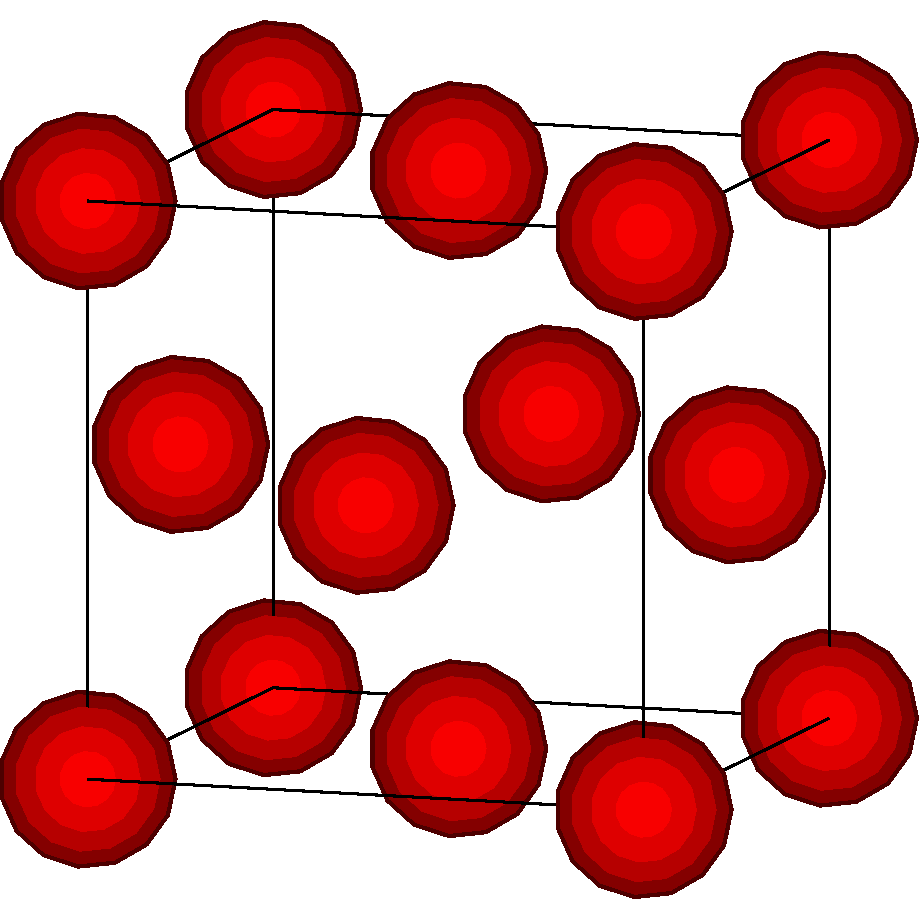
\includegraphics[width=\textwidth]{../assets/theorie/fcc}
        \caption{fcc-Gitter.} \label{fcc}
    \end{subfigure}
    \begin{subfigure}[t]{0.3\textwidth}
        \centering
        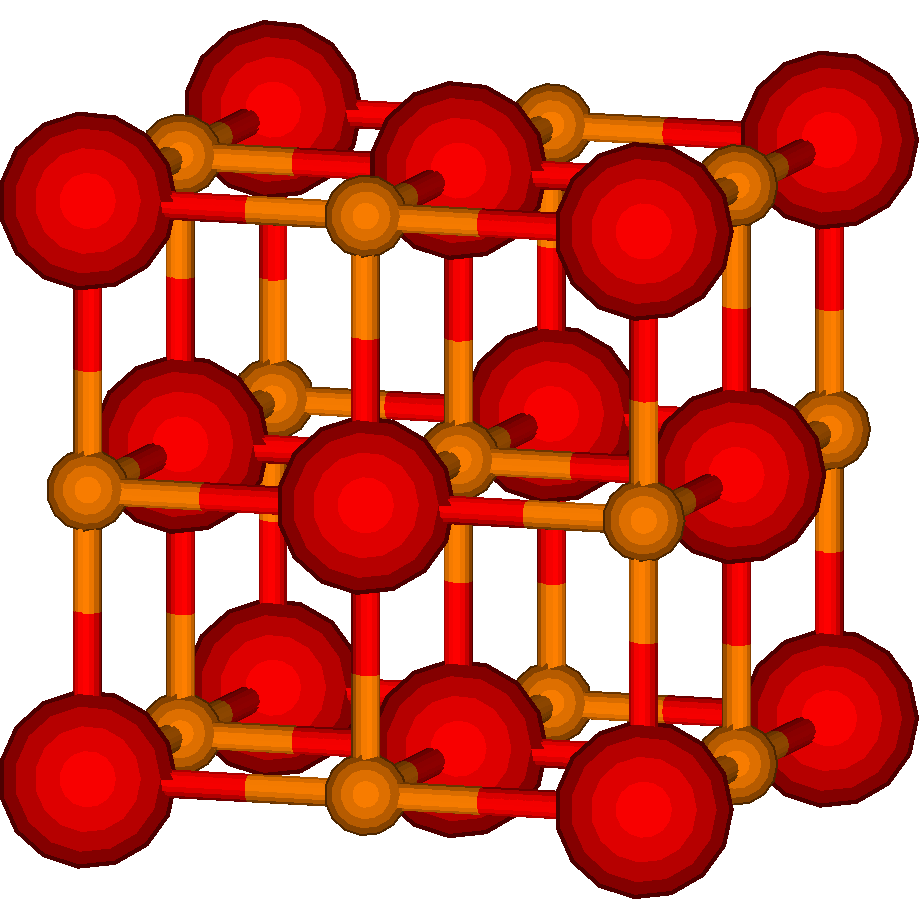
\includegraphics[width=\textwidth]{../assets/theorie/rocksalt}
        \caption{NaCl-Gitter} \label{nacl}
    \end{subfigure}
    \begin{subfigure}[t]{0.3\textwidth}
        \centering
        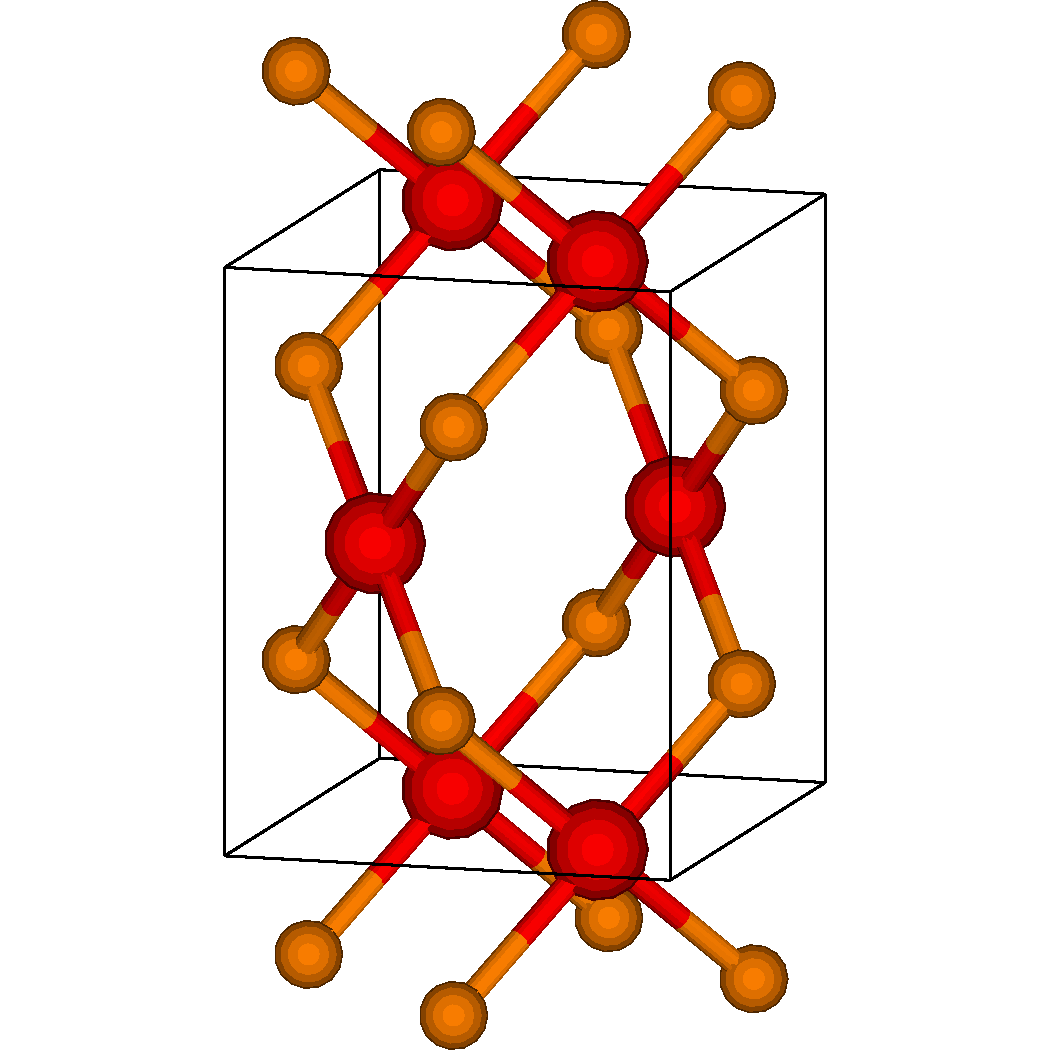
\includegraphics[width=\textwidth]{../assets/theorie/CuO}
        \caption{\ce{CuO}-Gitter} \label{cuo}
    \end{subfigure}
    \begin{subfigure}[t]{0.3\textwidth}
        \centering
        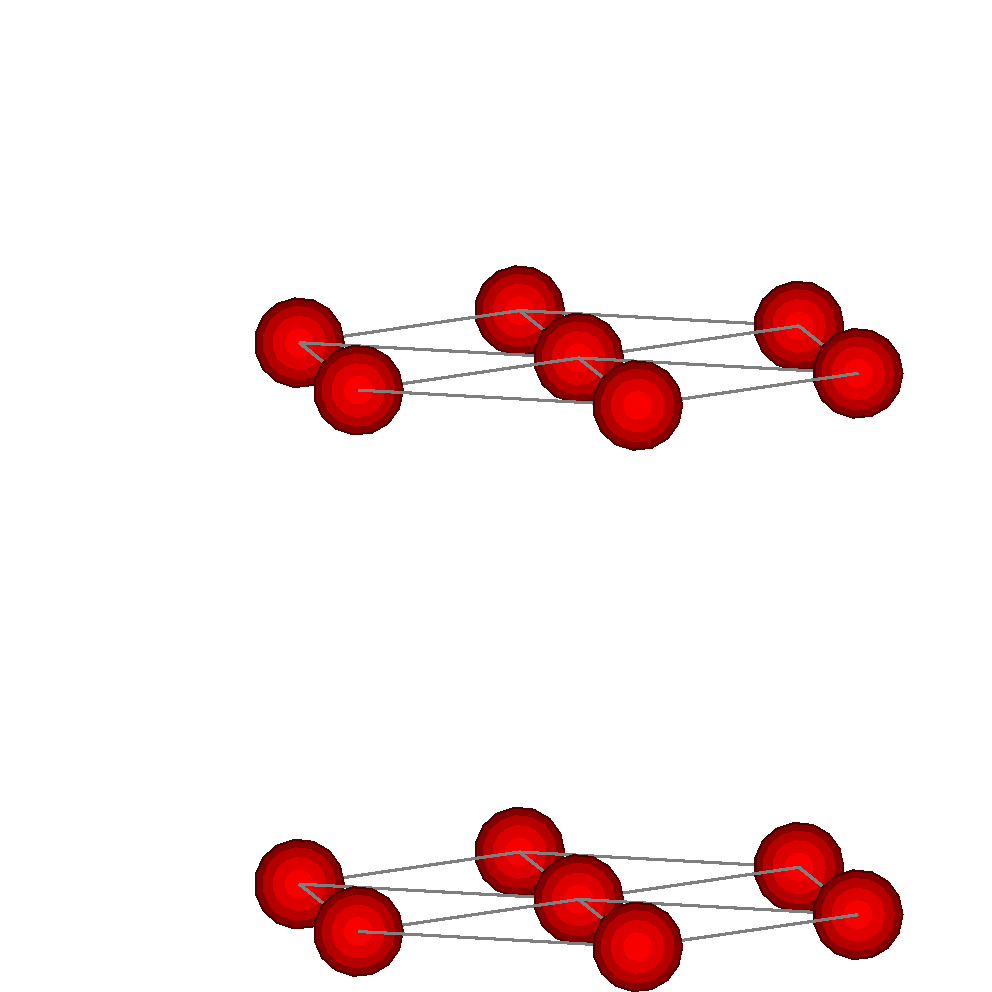
\includegraphics[width=\textwidth]{../assets/theorie/hex}
        \caption{hexagonales Gitter} \label{hex}
    \end{subfigure}
    \begin{subfigure}[t]{0.3\textwidth}
        \centering
        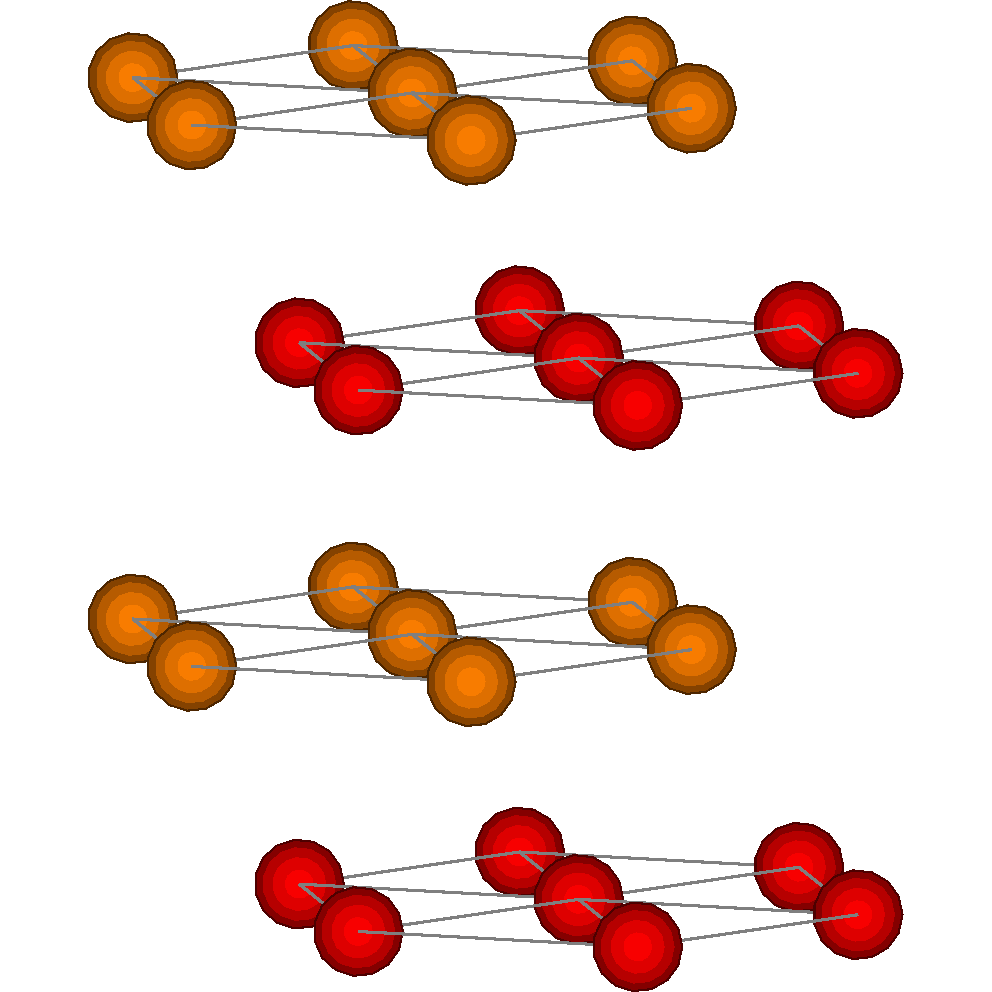
\includegraphics[width=\textwidth]{../assets/theorie/hcp}
        \caption{hcp-Gitter} \label{hcp}
    \end{subfigure}
    \begin{subfigure}[t]{0.3\textwidth}
        \centering
        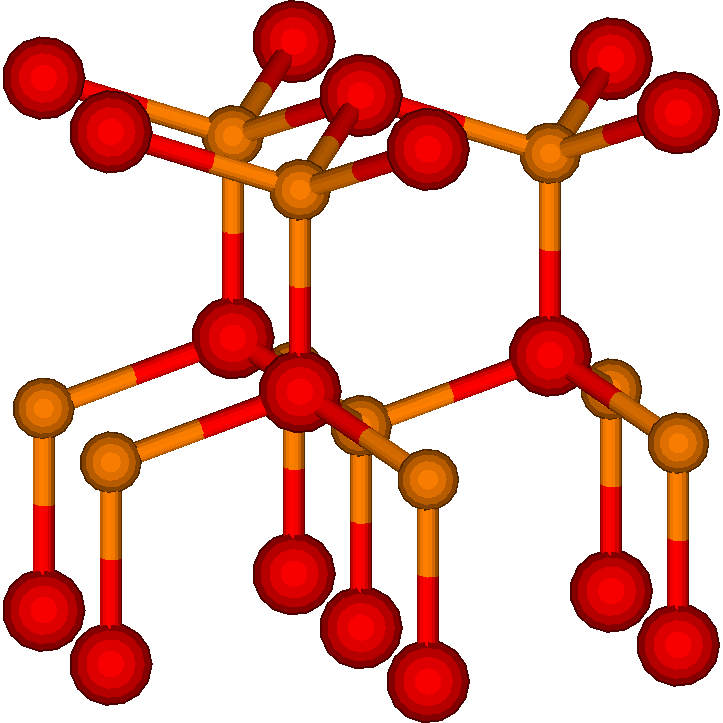
\includegraphics[width=\textwidth]{../assets/theorie/wurzite}
        \caption{Wurtzit-Gitter} \label{wurtzit}
    \end{subfigure}
    \caption{Ausgewählte Kristallgitter für die Untersuchung von \heo.} \label{fig:gitterstrukturen}
\end{figure}

\paragraph{Natriumchloridstruktur}
Die erste und wichtigste Kristallstruktur ist die Natriumchloridstruktur.
Um diese zu verstehen, betrachtet man zuerst ein kubisch-flächen\-zen\-trier\-tes Gitter (fcc, engl.
\textit{face-centered cubic}) welches durch die primitiven Vektoren
\begin{equation}
    \mathbf{a}_1 = a / 2 (\hat{x} + \hat{y}), \quad
    \mathbf{a}_2 = a / 2 (\hat{y} + \hat{z}), \quad
    \mathbf{a}_3 = a / 2 (\hat{x} + \hat{z})
    \label{eq:fcc}
\end{equation}
definiert ist \autocite{Grundmann}.
Die Gitterpunkte liegen an Würfelecken und den dazugehörigen Flächenmittelpunkten, wie in \cref{fcc} dargestellt.
Die Natriumchloridstruktur entsteht aus einem fcc-Gitter mit zweiatomiger Basis \autocite{Grundmann}.
Dabei ist das erste Basisatom an der Gitterposition $(0,0,0)$ und das zweite an der Position $(a/2,a/2,a/2)$, wie in
\cref{nacl} dargestellt.
Sowohl Magnesiumoxid (\ce{MgO}), Kobaltoxid (\ce{CoO}) und Nickeloxid (\ce{NiO}) kristallisieren in dieser Struktur.
Auch \heo\ kristallisiert in der Natriumchloridstruktur, wenn
Sauerstoff als erstes Basisatom und ein zufällig ausgewähltes Metall als zweites Basisatom betrachtet wird
\autocite{Rost2015}.

\paragraph{Tenoritstruktur}
Kupferoxid (\ce{CuO}) kristallisiert in einer monoklinen Kristall\-struk\-tur mit achtatomiger Basis.
Dabei sind vier dieser Basisatome Kupferatome und vier Sauerstoffatome.
Die Struktur ist in \cref{cuo} dargestellt \autocite{kupferoxid}.

\paragraph{Wurtzitstruktur}
Um die Wurtzitstruktur zu verstehen, betrachtet man zuerst die einfach-hexagonale Struktur, die durch die primitiven
Vektoren
\begin{equation}
    \mathbf{a}_1 = a\hat{x}, \quad
    \mathbf{a}_2 = a/2 (\hat{x} + \sqrt{3} \hat{y}), \quad
    \mathbf{a}_3 = c \hat{z}
    \label{eq:hex}
\end{equation}
definiert ist \autocite{Ashcroft}.
Es entsteht ein Gitter, welches an den Ecken eines Sechsecks und den dazugehörigen Flächenmittelpunkten Gitterpunkte
besitzt, wie in \cref{hex} dargestellt.
Aus der einfach-hexagonalen Struktur ergibt sich die hexagonal dichtest gepackte Struktur
(hcp, engl. \textit{hexagonal-closed packet}).
Dieser liegt ein einfach-hexagonales Gitter mit zweiatomiger Basis bei den Gitterpositionen $(0,0,0)$ und
$(\mathbf{a}_1/3 + \mathbf{a}_2/3 + \mathbf{a}_3/2)$ zugrunde, wie in \cref{hcp} dargestellt \autocite{Ashcroft}.
Die Wurtzitstruktur besteht aus einem einfach-hexagonalen Gitter mit vieratomiger Basis.
Eine bessere Vorstellung ergibt sich jedoch aus der Betrachtung zweier übereinander liegender hcp-Gitter, die um
die Höhe $\sqrt {3 / 8} a$ gegeneinander verschoben sind \autocite{Grundmann}, wie in \cref{wurtzit} dargestellt.
Zinkoxid (\ce{ZnO}) kristallisiert in dieser Struktur.

\subsubsection{Reziprokes Gitter}
Das reziproke Gitter spielt für die weitere Betrachtung periodischer Strukturen eine fundamentale Rolle.
Ziel ist es, eine Funktion zu konstruieren, die gitterperiodisch im Bravaisgitter ist.
Für diese Funktion soll also gelten
$f(\mathbf{x})=f(\mathbf{x}+\mathbf{O})$, falls $\mathbf{O}=\sum_{i=1}^{3} \alpha_{i}\mathbf{a}_{i}$.
Mithilfe einer Reihenentwicklung ergibt sich die folgende, allgemeine Form:
\begin{align}
    \begin{split}
        f(\mathbf{x})&=\sum_{\mathbf{R}}a_{\mathbf{R}}\cdot \exp(\mathrm{i}\mathbf{R}\cdot\mathbf{x}),\\
        f(\mathbf{x}+\mathbf{O})&=\sum_{\mathbf{R}}a_{\mathbf{R}}\cdot \exp(\mathrm{i}\mathbf{R}\cdot \mathbf{x})\cdot
        \underbrace{ \exp(\mathrm{i}\mathbf{R}\cdot \mathbf{O}) }_{ \stackrel{!}{=}1 }  \stackrel{!}{=} f(\mathbf{x}).
    \end{split}
\end{align}
Erkennbar ist die notwendige Bedingung $\exp(\mathrm{i}\mathbf{R}\cdot \mathbf{O})=1$.
Dies ist äquivalent zur Aussage $\mathbf{R}\cdot \mathbf{O}=2\pi z$ mit $z \in \mathbb{Z}$.
Mit dieser Vorbetrachtung ist es möglich, das reziproke Gitter durch die Menge
$\{ \mathbf{R} \,\vert\, \exp(\mathrm{i}\mathbf{R}\cdot \mathbf{O})=1 \quad
\forall \mathbf{O} \in \text{span}(\mathbf{a}_{i}) \}$ zu definieren \autocite{Ashcroft}.
Analog zum Ortsraum lassen sich auch hier primitiven Vektoren mit folgender Vorschrift bilden:
\begin{align*}
    \mathbf{b}_{1} = 2\pi \cdot \frac{\mathbf{a}_{2} \times \mathbf{a}_{3}}{V_{\mathrm{EZ}}} \quad
    \mathbf{b}_{2} = 2\pi \cdot \frac{\mathbf{a}_{3} \times \mathbf{a}_{1}}{V_{\mathrm{EZ}}} \quad
    \mathbf{b}_{3} = 2\pi \cdot \frac{\mathbf{a}_{1} \times \mathbf{a}_{2}}{V_{\mathrm{EZ}}}.
\end{align*}
Jeder Punkt im reziproken Gitter kann durch $\sum_{i=1}^{3} \beta_{i}\mathbf{b}_{i}$ mit $\beta_i \in \mathbb{Z},
i\in\{1,2,3\}$ beschrieben werden.
Es gilt die Relation $\mathbf{b}_{i}\cdot \mathbf{a}_{j}=2 \pi \delta_{ij}$.
Hierbei ist $\delta_{ij}$ das Kronecker-Delta \autocite{Ashcroft}.

\subsubsection{Indizierung von Gitterebenen und Gitterrichtungen}\label{subsubsec:indizierung}
Der Abschnitt orientiert sich an den Erkenntnissen von \citeauthoryear{Ashcroft} \autocite{Ashcroft}.

Die erste wichtige Anwendung des reziproken Gitters ist die Charakterisierung von Gitterebenen.
Eine Gitterebene ist eine beliebige, im Bravaisgitter liegende Ebene, die mindestens drei nicht kollineare Gitterpunkte
enthält.
Aufgrund der Kristallsymmetrie liegen damit unendlich viele weitere Gitterpunkte innerhalb dieser Ebene.
Mithilfe der Translationssymmetrie findet man parallele Gitterebenen im Abstand $d$.
Diese fasst man als Gitterebenenscharen zusammen.

Gitterebenenscharen kann man mithilfe des reziproken Gitters charakterisieren, denn für jede
Gitterebenenschar im Abstand $d$ existieren Vektoren des reziproken Gitters, welche senkrecht auf den Ebenen stehen.
Für die eindeutige Beschreibung wählt man den kleinsten dieser Vektoren $\mathbf{r}$, welcher stets die Länge $2 \pi / d$
besitzt.
Auch die Umkehrung gilt: Für jeden Vektor $\mathbf{R}$ aus dem reziproken Gitter, existiert eine Schar von senkrechten
Gitterebenen.
Der Abstand $d$ dieser Ebenen ist an den Betrag des zu $\mathbf{R}$ kleinsten parallelen Vektors $\mathbf{r}$ durch
$\lvert \mathbf{r}\rvert=2\pi  /d$ gekoppelt.
Somit existiert eine einfache Möglichkeit, Gitterebenen mithilfe von reziproken Gittervektoren eindeutig zu
identifizieren.

Um Gitterebenenscharen zu kennzeichnen, verwendet man die Millerschen Indizes.
Sei dazu $\mathbf{r}$ der kürzeste reziproke Gittervektor, welcher senkrecht auf der zu charakterisierenden Ebene steht.
Dieser lässt sich darstellen durch $ \mathbf{r} = h \mathbf{b_1} + k \mathbf{b_2} + l \mathbf{b_3}$.
Das Tupel $(h\, k\,l)$ sind die Millerschen Indizes, welche definitionsgemäß aus ganzen Zahlen bestehen müssen.

Es existiert eine geometrische Interpretation, die es erlaubt, die Indizes im Ortsraum zu
visualisieren.
Für jede Gitterebene findet man ein entsprechendes $A$, sodass die Ebenengleichung $\mathbf{r} \cdot \mathbf{x} = A$
erfüllt ist.
Nun definiert man die Durchstoßpunkte zwischen den durch die primitiven Vektoren $\mathbf{a}_i$ aufgespannten
Koordinatenachsen und der Ebene durch die Terme $x_{1}\mathbf{a}_{1}, x_{2}\mathbf{a}_{2}, x_{3}\mathbf{a}_{3}$.
Da die Durchstoßpunkte in der Ebene liegen, ist die Ebenengleichung $\mathbf{r}\cdot(x_{i}\mathbf{a}_{i})=A$ erfüllt und
man findet mit $\mathbf{r}\cdot\mathbf{a}_{1}=2\pi h$, $\mathbf{r}\cdot \mathbf{a}_{2}=2\pi k$,
$ \mathbf{r}\cdot \mathbf{a}_{3}=2\pi l$ folgenden Zusammenhang:
\begin{equation}
    x_{1}=\frac{A}{2\pi h}, \quad x_{2}=\frac{A}{2\pi k}, \quad x_{3} =\frac{A}{2\pi l}.
\end{equation}
Kennt man die Achsendurchstoßpunkte $x_i$, kann man die Millerschen Indizes finden, indem man den Parameter $A$
kleinstmöglich wählt, sodass $h$, $k$ und $l$ ganzzahlig sind.

Nicht nur Gitterebenen, sondern auch Gitterrichtungen lassen sich in ähnlicher Weise indizieren.
Das Tupel $[h\,k\,l]$ beschreibt diejenige Richtung, die durch den Vektor $\mathbf{O} = h\mathbf{a}_{1}+k\mathbf{a}_{2}+
l\mathbf{a}_{3}$ vorgegeben wird.
Zu beachten ist, dass Richtungsvektoren in diesem Kontext im Ortsraum leben,
währenddessen Ebenennormalenvektoren durch Vektoren im reziproken Raum dargestellt werden.
Um dies zu verdeutlichen, werden eckige anstelle der runden Klammern verwendet.
Es existiert weiterhin eine besondere Notation zur Kennzeichnung äquivalenter Gitterebenenscharen und Raumrichtungen.
In diesem Kontext bedeutet das, dass die Möglichkeit besteht, äquivalente Gitterebenenscharen und Raumrichtung durch
Symmetrieoperationen ineinander zu überführen.
Äquivalente Ebenen notiert man mit $\{h \,k\, l \}$, für Richtungen gilt entsprechend $\langle h\, k \, l \rangle$.

\subsubsection{Röntgenbeugung und die Laue Bedingung}
Ziel ist es, mithilfe elektromagnetischer Strahlung und den bisherigen Überlegungen, Aussagen über die
Kristallstruktur eines Festkörpers zu gewinnen.
Genauer gesagt sucht man einen Formalismus, um die elastische Streuung von Licht am Kristallgitter zu beschreiben.
Für eine geeignete Wellenlänge der Photonen betrachtet man die typische zwischenatomare Entfernung von circa
\qty{1}{\angstrom}.
Aus der Optik ist bekannt, dass mindestens eine Wellenlänge gleicher Größenordnung genutzt werden
muss, um beide Punkte hinreichend genau aufzulösen \autocite{Ashcroft}.
Entsprechend muss die Photonenenergie in der Ordnung von
$\h f =\h \c / \lambda \simeq \qty{12.3}{\electronvolt}$ liegen.
Hierbei ist $f$ die Frequenz, $\lambda$ die Wellenlänge, $\h$ das Plancksche Wirkungsquantum und $\c$ die
Lichtgeschwindigkeit.
Solche Energien sind charakteristisch für Röntgenstrahlung.

Laue und Bragg entwickelten zwei Formalismen, um elastischen Streuung elektromagnetischer Strahlung am Kristallgitter
zu beschreiben.
Im Folgenden wird der Laue-Formalismus erklärt und die Äquivalenz zur Bragg-Bedingung gezeigt.

\paragraph{Streuung an zwei Gitterpunkten}
\begin{figure}
    \centering
    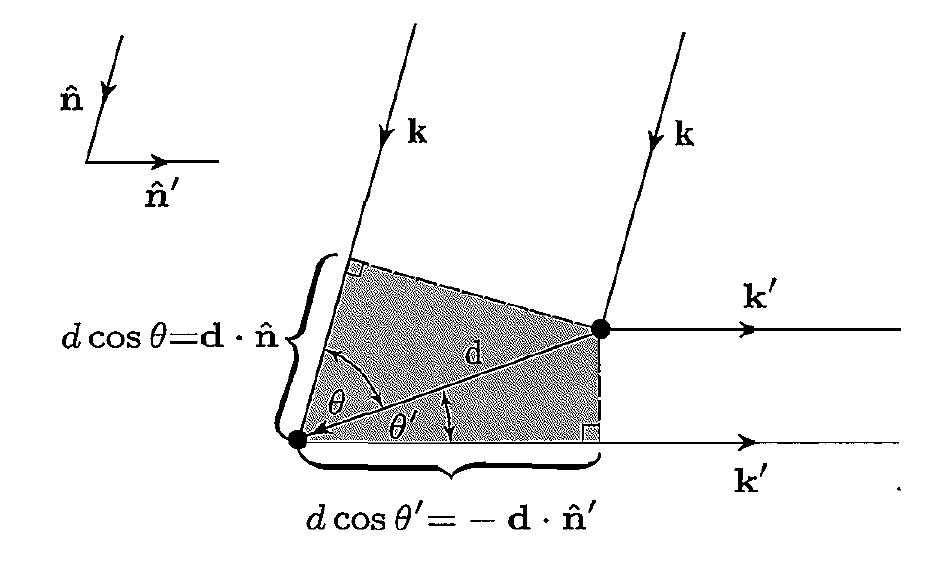
\includegraphics{../assets/theorie/lauebeugung}
    \caption{Skizze zur Erklärung der Laue-Bedingung. \imcitetwo{Ashcroft}} \label{fig:laue}
\end{figure}
Zur Herleitung der Beugungsbedingung nach Laue betrachtet man die Bestrahlung zweier Gitterpunkte mit Photonen unter
Annahme von elastischer Streuung.
Der Abstand der Gitterpunkte ist durch den Vektor $\mathbf{O}$ gegeben.
Dabei ist die einfallende Strahlung durch den Wellenzahlvektor  $\mathbf{k}$ charakterisiert.
Es gilt der Zusammenhang $\lvert \mathbf{k} \rvert = 2 \pi / \lambda$ und die Dispersionsrelation
$\omega = \c \lvert \mathbf{k} \rvert$.
Die gestreute Strahlung wird durch den Wellenzahlvektor $\mathbf{k}'$ beschrieben.
Da nur elastische Streuung betrachtet wird, gilt $\lvert \mathbf{k} \rvert=\lvert \mathbf{k}' \rvert$.
Somit sind die Frequenzen ($\omega$ und $\omega'$) beider Wellen gleich.
Für den Wegunterschied $\Delta s$ findet man anhand \cref{fig:laue} den Zusammenhang \autocite{Ashcroft}:
\begin{equation}
    \Delta s = \Delta s_{1} + \Delta s_{2} = \underbrace{ \mathbf{O} \cdot \frac{\mathbf{k}}{\lvert \mathbf{k} \rvert }
    -\mathbf{O}\cdot \frac{\mathbf{k}'}{\lvert \mathbf{k}' \rvert}  }_{\substack{\text{Projektion von } \\ \mathbf{O} \text{ auf }
    \mathbf{k} \text{ bzw. }\mathbf{k'} }} =  \frac{\lambda}{2\pi} \mathbf{O}\cdot\Delta \mathbf{k}.
    \label{eq:laue}
\end{equation}
Hierbei ist $\Delta \mathbf{k} = \mathbf{k}-\mathbf{k}'$ der Differenzvektor der Wellenzahlvektoren.
Für konstruktive Interferenz muss die Bedingung $\Delta s = n \lambda, n \in \mathbb{N}$ erfüllt sein, sodass durch
Gleichsetzen die Beziehung $\mathbf{O}\cdot\Delta \mathbf{k} =2\pi n$ folgt.
Aus der geometrischen Anordnung der Gitterpunkte ergibt sich ein Wegunterschied, der äquivalent
zu einer Phasendifferenz von $\Delta\varphi=(2\pi / \lambda) \cdot \Delta s = \Delta \mathbf{k}\cdot \mathbf{O}$ ist.

Unter der Annahme, dass beide Gitterpunkte Kugelwellen mit Amplituden $u_{0}(\mathbf{r})$ und $u_{1}(\mathbf{r})$
ausstrahlen, ergibt sich für die Überlagerung beider Wellen die folgende Form \autocite{Spiess}:
\begin{align}
    u(\mathbf{r},t)=u_{0}(\mathbf{r})\cdot \exp(\mathrm{i}\omega t+\mathrm{i}\lvert \mathbf{k}
    \rvert r) + u_{1}(\mathbf{r}) \cdot \exp(\mathrm{i}\omega t + \mathrm{i}\lvert \mathbf{k}
    \rvert r+\mathrm{i}\Delta\varphi).
\end{align}
Diese Überlagerung führt zu einer Interferenz, die durch die Phasendifferenz $\Delta\varphi$ bestimmt
wird.

\paragraph{Streuung an allen Gitterpunkten}
Will man die Streuung im gesamten Kristall betrachten, muss über alle Streuzentren, das heißt über alle Gittervektoren,
im Kristall summiert werden.
Diese sind gegeben durch $\mathbf{O}_{pqr}=p\mathbf{a}_{1}+q\mathbf{a}_{2}+r\mathbf{a}_{3}$.
Für die Superposition aller Wellen mit Amplitude $u_{pqr}(\mathbf{r})$ und Phasendifferenz $\Delta\varphi_{pqr}$
ergibt sich:
\begin{align}
    \begin{split}
        u(\mathbf{r}, t)
        &=\sum_{pqr} u_{pqr}(\mathbf{r})\cdot \exp(\mathrm{i}\omega t+\mathrm{i}
        \lvert \mathbf{k} \rvert r+\mathrm{i}\underbrace{ \Delta\varphi_{pqr} }_{ = \Delta
        \mathbf{k}\cdot \mathbf{O}_{pqr}})) \\
        &=\exp(\mathrm{i}\omega t+\mathrm{i}\lvert \mathbf{k} \rvert r)\cdot
        \underbrace{ \sum_{pqr}u_{pqr}(\mathbf{r})\cdot \exp(\mathrm{i}\Delta \mathbf{k}
        \cdot \mathbf{O}_{pqr}) }_{ \coloneqq A }.
    \end{split}
    \label{eq:amplitude}
\end{align}
Die Größe $A$ wird als Streuamplitude bezeichnet.
Die tatsächliche Streuung erfolgt an der Elektronenverteilung.
Das führt zu zusätzlichen Effekten wie dem Atomformfaktor und dem Strukturfaktor,
welche für weitere Betrachtungen jedoch vernachlässigt werden können \autocite{Spiess}:
\begin{equation}
    A \propto \int n(\mathbf{r}) \exp(\mathrm{i} \Delta \mathbf{k}\cdot
    \mathbf{r}) \, \mathrm{d}V(\mathbf{r}).
    \label{eq:atomformfaktor}
\end{equation}

\paragraph{Beugungsbedingung}
Die Bedingung für konstruktive Interferenz ist äquivalent zur Maximierung der Streuamplitude.
Damit diese maximal wird, muss die Interferenzbedingung $\mathbf{O}_{pqr}\cdot\Delta \mathbf{k} =2\pi z$
für alle $p$, $q$, $r$ gelten.
Zerlegt man $\mathbf{O}_{pqr}$ in seine Komponenten, erhält man folgende Gleichungen:
\begin{equation}
    \mathbf{a}_{1}\cdot\Delta \mathbf{k} = 2\pi h, \quad
    \mathbf{a}_{2}\cdot\Delta \mathbf{k} = 2\pi k, \quad
    \mathbf{a}_{3}\cdot\Delta \mathbf{k} = 2\pi l
    \label{eq:lauebedingung}
\end{equation}
Dies sind die Laue Gleichungen für Beugungsmaxima.
Sie sind erfüllt, falls $\Delta \mathbf{k}$ ein reziproker Gittervektor ist.
Es stellt die Beugungsbedingung nach Laue dar, die besagt, dass konstruktive Interferenz genau dann auftritt,
wenn $\Delta \mathbf{k}$ einem Vektor des reziproken Gitters entspricht \autocite{Ashcroft}.

Für die Strukturamplitude ergibt sich anschließend:
\begin{equation}
    A = \sum_{pqr} u_{pqr}(\mathbf{r}) \cdot\underbrace{ \exp(2\pi \mathrm{i}
    \cdot(\underbrace{ mh+nk+pl }_{ \in\mathbb{Z} })) }_{ =1 }
    = \sum_{pqr} u_{pqr}(\mathbf{r}).
    \label{eq:strukturamplitude}
\end{equation}

\paragraph{Bragg-Bedingung}
Die Bragg Bedingung kann sowohl mithilfe der Laue-Bedingung als auch geometrisch hergeleitet werden.
Um die Äquivalenz zur Laue-Bedingung zu zeigen, wird die Bragg-Bedingung im Folgenden aus der Laue-Bedingung
hergeleitet.
Betrachtet man einen Differenzvektor $\Delta \mathbf{k}=\mathbf{k}'-\mathbf{k}$, wobei $\mathbf{k}$ und
$\mathbf{k'}$ den Winkel $\alpha$ einschließen,so ist sein Betrag gegeben durch:
\begin{align}
    \begin{split}
        \lvert \Delta \mathbf{k} \rvert ^{2}&=\langle \Delta \mathbf{k} ,\Delta \mathbf{k}\rangle =\langle
        \mathbf{k}-\mathbf{k}', \mathbf{k}-\mathbf{k}' \rangle = k^{2}+k'^{2}-2kk'\cos(\alpha)  \\
        &=2{k}^{2}(1-\cos(\alpha))=4k^{2}\sin ^{2}\left( \frac{\alpha}{2} \right)
        =4k^{2}\sin ^{2}( \nu).
    \end{split}
\end{align}
Hierbei ist $\nu = \alpha / 2$ der Bragg-Winkel und $\langle \cdot , \cdot \rangle$ das Standardskalarprodukt.
Da $\Delta \mathbf{k}$ ein Vektor aus dem reziproken Raum ist und senkrecht auf der Gitterebene
steht, an welcher er gestreut wird, existiert ein kürzester Vektor $\mathbf{g}$, sodass
$n\cdot \mathbf{g} =\Delta \mathbf{k}$.
Aus \cref{subsubsec:indizierung} ist bekannt, dass $\mathbf{g}$ den Abstand der Netzebenen definiert
mit $d = 2 \pi \cdot\lvert \mathbf{g} \rvert ^{-1}$.
Daraus folgt $\lvert \Delta \mathbf{k} \rvert=n \lvert \mathbf{g} \rvert = 2\pi n/d$.
Kombiniert man beide Gleichungen miteinander, ergibt sich die Bragg-Bedingung \autocite{Ashcroft}:
\begin{align}
    \begin{split}
        2k\sin(\nu)&=\frac{2\pi n}{d}, \\
        2d\sin(\nu)&=n \lambda.
    \end{split}
\end{align}

\subsection{Entropiestabilisierte Metalloxide}\label{subsec:hochentropische-metalloxide}
\begin{figure}
    \centering
    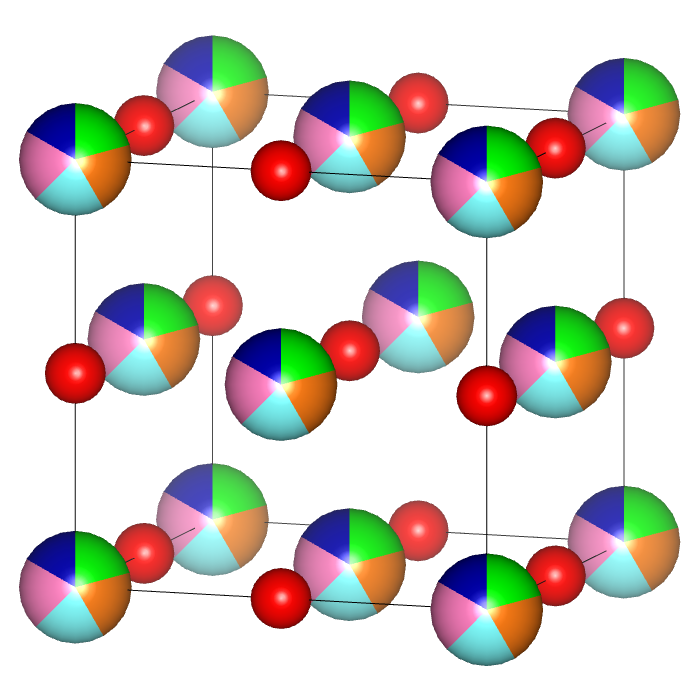
\includegraphics[width=0.3\textwidth]{../assets/theorie/heo}
    \caption{Struktur von \heo. Rot: Sauerstoff, Bunt: Metallkationen.}
    \label{fig:heo}
\end{figure}
Wie bereits in \cref{sec:einleitung} erwähnt, haben \citeauthoryear{Rost2015} eindrucksvoll eine neue Klasse von
Materialien vorgestellt, die sogenannten entropiestabilisierten Metalloxide.
Obwohl in dieser Arbeit mit Dünnfilmen gearbeitet wird, deren Eigenschaften nicht identisch mit den korrenspodierenden
Massivmaterialien sind, bietet die Forschung von \citeauthoryear{Rost2015} wertvolle Einblicke und
Vergleichsmöglichkeiten.
Im Folgenden wird aus diesem Grund die Synthese und Struktur von \heo\,-Pellets
sowie die zugrundeliegende Theorie
der Entropiestabilisierung erläutert.

\subsubsection{Synthese und Struktur von \texorpdfstring{\heo}{MgCoNiCuZnO}}\label{subsubsec:heo}
Für die Herstellung von \heo\ wurden von \citeauthoryear{Rost2015} die einzelnen binären Oxidpulver \ce{MgO}, \ce{CoO},
\ce{NiO}, \ce{CuO} und \ce{ZnO} zu äquimolaren Anteilen gemahlen, in Pellets gepresst und anschließend bei den
Temperaturen \qtylist{750;800;850;900;1000}{\celsius} für \qty{2}{\hour} gesintert.
Anschließend wurden die Proben durch direkte Extraktion aus dem Ofen auf Raumtemperatur abgekühlt.
Nach jedem Ausheizprozess wurde die Kristallinität durch Röntgendiffraktometrie untersucht.
Die Diffraktogramme sind in \cref{fig:rost1} dargestellt.
Bei den Temperaturen \qtylist{750;800;850}{\celsius} wurden mithilfe von $2\theta/\omega$-Diffraktogrammen die
Natriumchloridstruktur und die Tenoritstruktur identifiziert.
Vollständige Transformation in die Natriumchloridstruktur erfolgte zwischen \qty{850}{\celsius} und \qty{900}{\celsius}.

\citeauthoryear{Rost2015} stellen weitere Proben her, um die Rolle der Entropie im Bezug zur Phasenübergangstemperatur
zu charakterisieren.
Für jedes Metallkation wurde eine Serie von Proben synthetisiert, in der die Konzentration $X$ des jeweiligen
Metallkations zwischen \qty{10}{\percent} und \qty{30}{\percent} variierte und die Konzentrationen der anderen
Metallkationen äquimolar verteilt waren.
Erneut wurde die Kristallinität durch Röntgendiffraktometrie untersucht
und die Übergangstemperatur zur Einzelphase als Funktion der Konzentration $X$ bestimmt, siehe \cref{fig:rost2}.
Erkennbar ist, dass die Übergangstemperaturen zur Einzelphase steigen, sobald sich der Abstand $\lvert X-0.2 \rvert$
vergrößert.

\captionsetup{justification=justified}
\begin{figure}
    \centering
    \begin{subfigure}{0.9\textwidth}
        \centering
        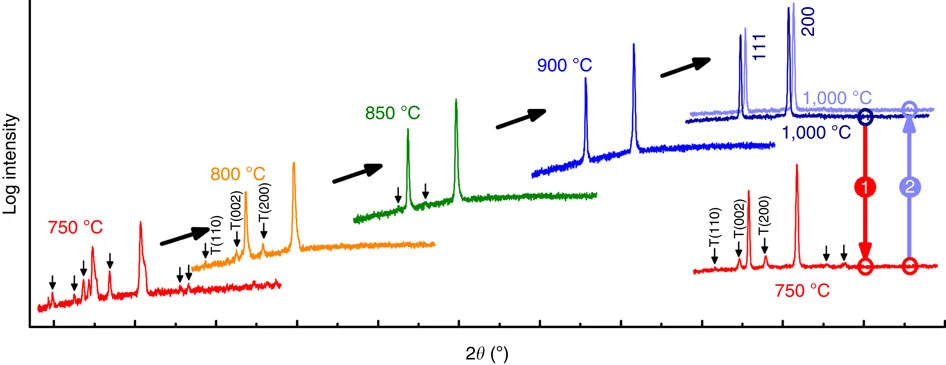
\includegraphics[width=\textwidth]{../assets/theorie/rost1}
        \caption{$2 \theta/\omega$ Diffraktogramme für \heo\ zu ausgewählten Temperaturen.
        Die Röntgenintensität ist logarithmisch aufgetragen und Pfeile zeigen auf Peaks, die mit Nicht-Natriumchloridphasen
        assoziiert sind, Peaks mit (T) und (RS) indiziert entsprechen Tenorit- bzw. Natriumchloridphasen.
        Die beiden Röntgenmuster für \qty{1000}{\degreeCelsius} geglühte Proben sind zur besseren Übersicht in
            $2\theta$ verschoben.}
        \label{fig:rost1}
        \vspace*{10mm}
    \end{subfigure}
    \begin{subfigure}{0.6\textwidth}
        \centering
        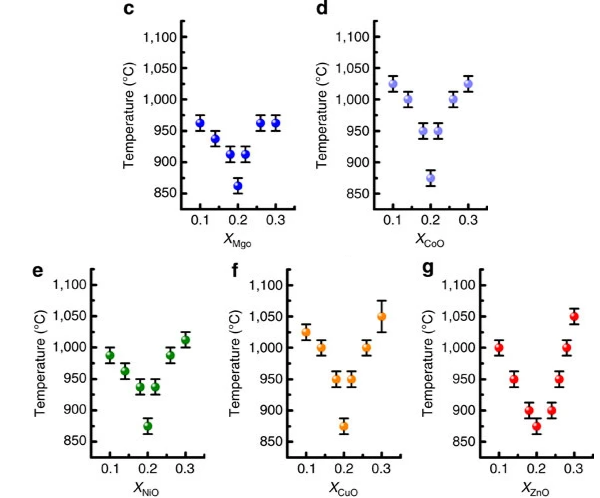
\includegraphics[width=\textwidth]{../assets/theorie/rost2}
        \caption{Partielle Phasendiagramme, welche die Übergangstemperatur zur Einzelphase als Funktion der Komposition
        in der Nähe der äquimolaren Zusammensetzung zeigen, wo maximale Konfigurationsentropie erwartet wird.
        Fehlerbalken berücksichtigen die Unsicherheit zwischen Temperaturintervallen. Jedes Phasendiagramm variiert
        systematisch die Konzentration eines Elements.}
        \label{fig:rost2}
        \vspace*{10mm}
    \end{subfigure}
    \caption{Auszüge aus der Arbeit von \citeauthoryear{Rost2015} \autocite{Rost2015}.}
\end{figure}
\captionsetup{justification=centering}

Diese ersten beiden Experimente weisen darauf hin, dass die Entropie eine entscheidende Rolle für die Stabilität von
\heo\ spielt.
Um dessen Struktur auf atomarer Ebene zu charakterisieren, wurden von \citeauthoryear{Rost2015} EXAFS-Messungen
und STEM-EDX Untersuchungen durchgeführt.
Die Ergebnisse legen nahe, dass \heo, in Analogie zu den HEAs, ein Mehrkomponentenoxid ist, welches in einer
Natriumchloridstruktur kristallisiert.
Dabei wird die Kationenstelle durch ein zufälliges Metallkationen \ce{Mg^{2+}}, \ce{Co^{2+}}, \ce{Ni^{2+}},
\ce{Cu^{2+}} oder \ce{Zn^{2+}} besetzt.
Im Kontrast zu den HEAs existiert ein geordnetes Anionengitter, welches durch Sauerstoffionen besetzt ist.
Die Struktur von \heo\ ist in \cref{fig:heo} dargestellt.

Es ist bemerkenswert, dass diese Phase stabil synthetisiert werden konnte, insbesondere angesichts der Änderungen in der
Kristallstruktur von \ce{ZnO} und \ce{CuO} sowie der damit verbundenen positiven Enthalpie.
Um dieses Phänomen zu verstehen, muss die Rolle der Gibbs-Energie und der darin auftretenden Entropie
erläutert werden.

\subsubsection{Gibbs-Energie und Phasenstabilität}
Aus der Thermodynamik ist bekannt, dass ein Prozess genau dann freiwillig abläuft, falls die Gesamtentropie des
Systems und seiner Umgebung zunimmt.
Beschränkt man sich auf Prozesse, die bei konstantem Druck und Temperatur ablaufen, dann ist diese Aussage äquivalent
zur Minimierung der Gibbs-Energie $G$, welche in der einfachsten Betrachtung folgendermaßen definiert ist
\autocite{Demtrder2015}:
d\begin{align}
    \begin{split}
        G(T,p, \{ n_{i} \})&=H(T,p,\{ n_{i} \})-TS(T,p,\{ n_{i} \}), \\
        \Delta G(T, p, \{ n_{i} \})&=\Delta H(T,p, \{ n_{i} \})-T \Delta S(T,p, \{ n_{i} \})
    \end{split}
    \label{eq:gibbs}
\end{align}
Hierbei ist $H$ die Enthalpie, $S$ die Entropie, $T$ die Temperatur, $p$ der Druck und $n_{i}$ die Stoffmengen jener
Komponenten, die am Prozess beteiligt sind.
Das $\Delta$ symbolisiert die Änderung der jeweiligen Größe bei Betrachtung zweier Zustände.
Die Gibbs-Energie ist eine Zustandsgröße und hängt nur von den Größen $T$, $p$ und $\{ n_{i} \}$ ab.
Die Änderung der Gibbs Energie $\Delta G$ ist ein Maß für die Spontanität eines Prozesses.
Ist $\Delta G < 0$, so läuft der Prozess freiwillig in einen energetisch günstigeren Zustand ab \autocite{rost_phd}.
Aus dieser Forderung ist ersichtlich, dass der stabilste Zustand die Gibbs-Energie minimiert.

Die Gibbs-Energie ist maßgeblich von der Enthalpie, der Temperatur und der Entropie abhängig.
Für niedrige Temperaturen wird die Gibbs-Energie nahezu ausschließlich durch die Enthalpie bestimmt.
Nicht selten sind Enthalpie-minimierte Zustände diejenigen, die auch die Gibbs-Energie minimieren.
Für hochentropische Materialien ist das in der Regel nicht der Fall.
Diese zeichnen sich dadurch aus, dass sie eine hohe Entropie besitzen, sodass das System
bei entsprechend hohen Temperaturen in einen anderen, als den Enthalpie-minimalen Zustand übergeht \autocite{Rost2015}.
Dieser Zustand ist dann durch die Entropie stabilisiert.

\subsubsection{Mischungsentropie}
Die Entropie ist von zentrale Bedeutung in der Stabilität von hochentropischen Materialien.
Für diese Beschreibung zieht man das Modell der idealen Lösung heran.
Dies ist eine Mischung aus zwei oder mehreren Komponenten, deren Mischung nicht mit einer Änderung der
Wärme oder Volumenänderung verbunden ist \autocite{DeHoff2006}.
Dabei wird die Entropie der Mischung mithilfe der Mischungsentropie von Idealgasen beschrieben.
Für diese findet man die folgende Form \autocite{rost_phd}:
\begin{equation}
    \Delta S_{\text{Misch}} = -\mathrm{R} \sum_{i=1}^N x_{i} \ln(x_{i}).
    \label{eq:Mischungsentropie}
\end{equation}
Hierbei ist $\mathrm{R}$ die allgemeine Gaskonstante, $x_{i}$ die Stoffmengenanteile der Komponenten und $N$ die Anzahl
der Komponenten.
Das Maximum der Entropie wird erreicht, wenn alle Komponenten gleichmäßig verteilt sind.
Dann gilt $x_{i}=1/N$ und $\max(S_{\text{Misch}}) = \mathrm{R} \ln(N)$.

Eine weitere Möglichkeit zur Visualisierung der Mischungsentropie ergibt sich, indem man die Konzentration eines
Konstituenten variiert und alle anderen äquimolar verteilt.
Mit der Parametrisierung $x_{1} = x$ und $x_{j} = (1-x) / (N-1)$ für $j=2, \dots, N$ ergibt sich für die
Mischungsentropie \autocite{Rost2015}:
\begin{equation}
    \Delta S_{\text{Misch}} = -R \left( x \ln(x) + (1-x) \ln \left( \frac{1-x}{N-1} \right) \right).
    \label{eq:Mischungsentropie2}
\end{equation}
\begin{figure}
    \centering
    \import{../plots/theory}{mixing_entropy.pgf}
    \caption{Darstellung der Mischungsentropie in Abhängigkeit der Konzentration bei $N$ Komponenten und Variation einer
    Komponente unter äquimolarer Verteilung der übrigen Komponenten.
    Das Maxima der Mischungsentropie wird erreicht, wenn alle Komponenten gleichmäßig verteilt sind.
    \imcitetwo{Rost2015}}
    \label{fig:Mischungsentropie}
\end{figure}

Diese ist in \cref{fig:Mischungsentropie} dargestellt.
Hieraus ist erneut erkennbar, dass die Mischungsentropie maximal wird, wenn alle Komponenten äquimolar verteilt sind.

Im Bezug auf die Gibbs-Energie impliziert dies, das die für den Phasenübergang nötige Temperatur umso niedriger sein
kann, je höher die Mischungsentropie ist.
Für eine äquimolare Verteilung ist die geringste Temperatur notwendig, um den Phasenübergang zu erreichen.
Aus diesem Grund wurden die Komponenten in \heo\ äquimolar verteilt.

\subsubsection{Ideale und reale Lösungen}
Mithilfe der idealen Lösung konnte die Mischungsentropie von \heo\ beschrieben werden.
Problem ist, dass in diesem Modell die Enthalpie der Mischung nicht verändert wird.
Für die ideale Lösung gilt $\Delta H_\mathrm{Misch} = 0$.
In der Realität ändern sich jedoch Bindungsenergien der Atome.
Wie in \cref{subsubsec:kristallgitter} erläutert, kristallisiert $\ce{CuO}$ in der Tenoritstruktur, $\ce{ZnO}$ in der
Wurtzitstruktur wohingegen \heo\ in der Natriumchloridstruktur kristallisiert.
Auch die übrigen Konstituenden ändern ihre Gitterkonstanten leicht.
Die Änderungen solcher Bindungsenergien ändern die Enthalpie der Mischung und damit auch die Gibbs-Energie.
Um eine Erweiterung zu finden, die auch die Enthalpie der Mischung berücksichtigt, betrachtet man ein
Zweikomponentensystem, welches gemischt wird:
\begin{equation}
    \mathrm{A} + \mathrm{B} \longrightarrow \mathrm{AB}.
    \label{eq:reaktion}
\end{equation}
Die Mischungsentropie ist nach vorherigem Abschnitt gegeben durch:
\begin{equation}
    \Delta S_{\mathrm{mix}}=-R[x_{\mathrm{A}}\ln(x_{\mathrm{A}})+x_{\mathrm{B}}\ln(x_{\mathrm{B}})].
    \label{eq:Mischungsentropie3}
\end{equation}
Im einfachsten Modell einer realen Lösung besitzt die Mischungsenthalpie die Form \autocite{rost_phd}:
\begin{equation}
    \Delta H_{\mathrm{Misch}}= a x_{\mathrm{A}} x_{\mathrm{B}}.
    \label{eq:Mischungsenthalpie}
\end{equation}
Hierbei ist $a$ eine Konstante, die die Bindungsenergie der Mischung beschreibt.
Unter dieser Annahme wird die Enthalpie eine Kompositionsfunktion.
Je nach Vorzeichen von $a$ können entweder gleichatomige Bindungen ($a > 0$) oder ungleichatomige Bindungen
($a < 0$) enthalpisch bevorzugt sein.
In den meisten Fällen ist $a > 0$, da energetisch ungünstigere Bindungen durch die Mischung entstehen.
Der Sonderfall $a=0$ entspricht der idealen Lösung.
Somit kann eine Erweiterung der Änderung der Gibbs-Energie gefunden werden \autocite{rost_phd}:

\begin{equation}
    \Delta G_{\mathrm{Misch}}=\Delta H_{\mathrm{Misch}}-T\Delta S_{\mathrm{Misch}}=a x_{\mathrm{A}} x_{\mathrm{B}}
    +RT[x_{\mathrm{A}}\ln(x_{\mathrm{A}})+x_{\mathrm{B}}\ln(x_{\mathrm{B}})].
    \label{eq:mischgibbs}
\end{equation}

\begin{figure}
    \centering
    \import{../plots/theory}{mixing_properties.pgf}
    \caption{Darstellung von Mischungsenthalpie, Mischungsentropie und Gibbs Energie der Mischung in Abhängigkeit der
    Konzentration.
    \imcitetwo{rost_phd}}
    \label{fig:mixing_properties}
\end{figure}

Diese Änderung, zusammen mit Enthalpie- und Entropieänderung, ist in \cref{fig:mixing_properties} dargestellt.
Es ist zu erkennen, dass für niedrige Temperaturen die Gibbs-Energie nahezu ausschließlich durch die Enthalpie bestimmt
wird
Das Minimum bei $x=0$ beziehungsweise $x=1$ weist darauf hin, dass die Gibbs-Energie minimal ist, wenn die
Komponenten rein sind.
Erst mit steigender Temperatur beginnt die Mischungsentropie einen Einfluss auf die Gibbs-Energie zu nehmen.
Dies sorgt für eine stabile Mischphase bei hohen Temperaturen, sodass das Minimum der Gibbs-Energie bei $x=0.5$ liegt.
    %\section{Probenherstellung und Messmethoden}\label{sec:messmethoden}

\subsection{Gepulste Laserabscheidung}\label{subsec:pld}
\begin{figure}
    \centering
    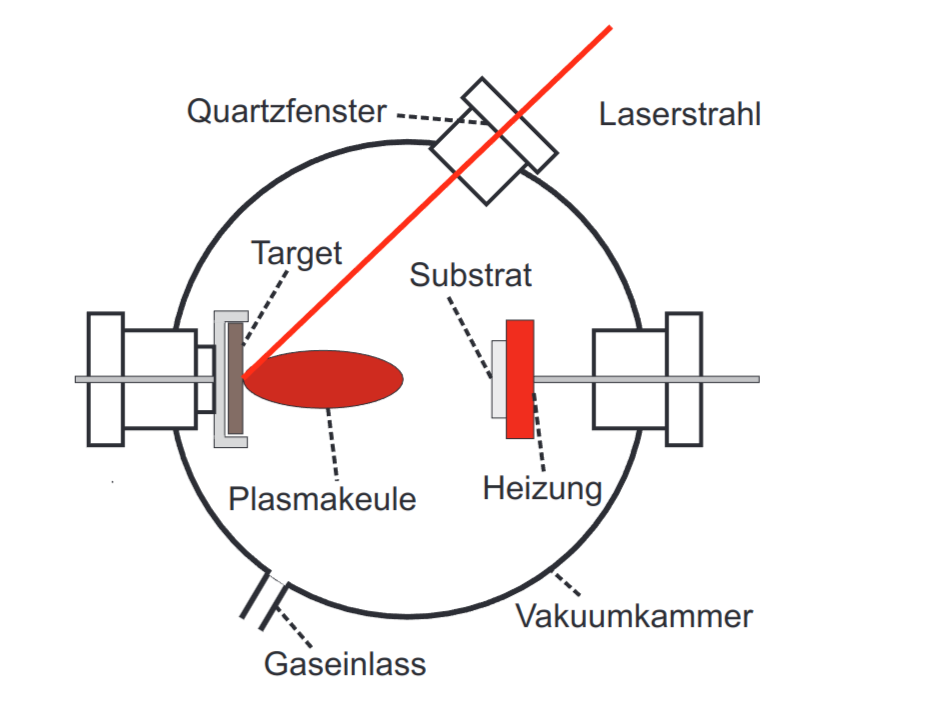
\includegraphics[width=0.6\textwidth]{../assets/messmethoden/pld/aufbau}
    \caption{Schematischer Aufbau eines PLD-Systems. \imcite{Lorenz2019}}
    \label{fig:pld}
\end{figure}
Die im Rahmen dieser Arbeit betrachteten Dünnfilme wurden mithilfe der gepulsten Laserabscheidung
(PLD, engl. \textit{pulsed laser deposition}) hergestellt.
Dafür wird ein hochenergetischer, gepulster Laserstrahl auf ein Target in einer Vakuumkammer abgebildet, welches bei
hinreichender, materialabhängiger Energie beginnt zu schmelzen und zu verdampfen.
Durch die Wechselwirkung der herausgelösten Atome mit den Laserpulsen entsteht eine Plasmawolke, die sich senkrecht
zum Target ausbreitet.
Die Plasmawolke expandiert in der Vakuumkammer und kann auf einem passend platzierten Substrat abgeschieden werden.
Der schematische Aufbau eines PLD-Systems ist in \cref{fig:pld} dargestellt.
Im Folgenden soll dieser Mechanismus genauer beschrieben werden.
Dabei orientiert sich dieser Abschnitt an \citeauthoryear{Lorenz2019} \autocite{Lorenz2019}.

Bevor ein PLD Prozess gestartet werden kann, muss ein geeignetes Target ausgewählt werden,
indem die einzelnen Binäroxidpulver im äquimolaren Verhältnis abgewogen, in einer Kugelmühle gemahlen,
in eine zylindrische Form gepresst und anschließend für \qty{12}{\hour} bei \qty{1000}{\celsius} gesintert werden.
Anschließend kann es im Targethalter montiert werden.

Der gesamte Prozess findet in einer Vakuumkammer statt, welche exemplarisch in \cref{fig:pld_kammer} dargestellt ist.
Durch Vor- und Turbomolekularpumpen kann ein Vakuum in der Größenordnung von \qty{e-5}{\milli\bar} erzeugt werden.
Zusätzlich können auch Hintergrundgase, unter anderem Sauerstoff und Stickstoff, in die Kammer eingelassen werden.

Um einen PLD Prozess zu starten, muss vorher das Hintergrundgas und dessen Druck in der Vakuumkammer eingestellt werden.
Außerhalb der Vakuumkammer generiert ein \ce{KrF}-Excimerlaser Laserpulse mit einer Wellenlänge von
\qty{248}{\nano\meter}.
Diese Laserpulse werden durch ein Fenster in die Vakuumkammer geleitet und auf das Target abgebildet.
Sie werden anschließend vom Target absorbiert und regen Elektronen der Targetkonstituenten an, die durch
Elektron-Phonon-Wechselwirkung in thermische, chemische und mechanische Energie umgewandelt werden.
Das führt zur Erhitzung des Targets, welches schmilzt und verdampft.
Da das Target durch den Laserstrahl nur an einer kleinen Stelle erhitzt wird, ist es notwendig,
dass sich das Target relativ zum Laserstrahl bewegt, um eine gleichmäßige Abtragung zu gewährleisten.
Dies erfolgt durch Rotations- und Translationsbewegungen.

\begin{figure}
    \centering
    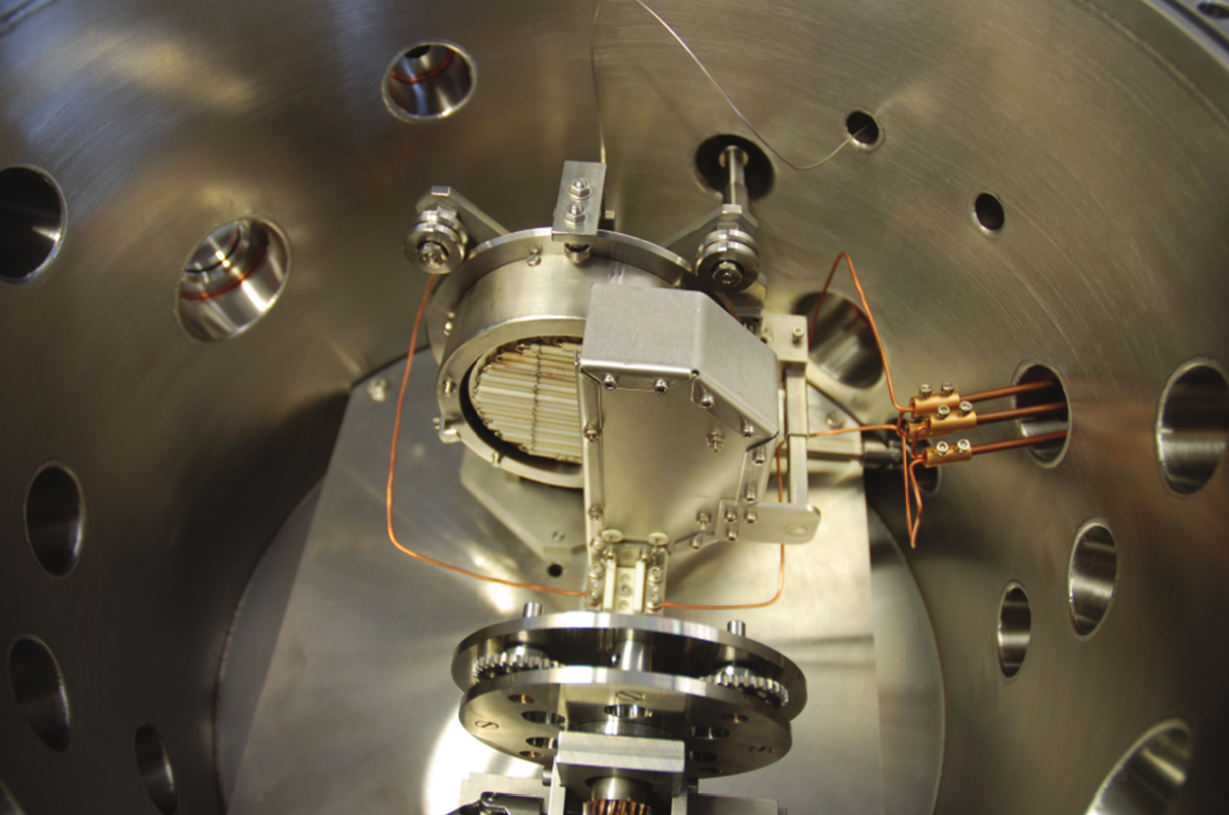
\includegraphics[width=0.6\textwidth]{../assets/messmethoden/pld/kammer}
    \caption{Innenansicht der PLD-Kammer. \imcite{Lorenz2019}}
    \label{fig:pld_kammer}
\end{figure}

Die verdampften Konstituenten interagieren ebenfalls mit den Laserphotonen und bilden durch Photoionisation eine
Plasmawolke, die sich in der Vakuumkammer ausbreitet.
Diese expandiert in der Vakuumkammer senkrecht zum Target.
Das Hintergrundgas in der Vakuumkammer interagiert mit der Plasmawolke durch Stoßprozesse.
Da der Substrathalter gegenüber vom Target positioniert ist, scheiden sich Anteile der Plasmawolke auf dem
Substrat ab.
Es beginnt ein Adsorptionsprozess, sodass sich ein Dünnfilm auf dem Substrat bildet.

Für die Arbeit wurden $\qty{10}{\milli\meter} \times \qty{10}{\milli\meter}$ Corning Eagle-XG-Glassubstrate verwendet.
Dies ist ein amorphes Glas, welches über eine hohe thermische Stabilität verfügt.
Da Phasenübergänge und Kristallisationsprozesse beobachtet werden sollen, ist es notwendig, ein Substrat zu wählen,
welches möglichst wenig Struktur auf die Dünnfilme überträgt.
\newpage
\subsection{Ausheizmethoden}\label{subsec:ausheiz}

\paragraph{Vakuumkammer}
\begin{figure}
    \centering
    \begin{subfigure}{0.35\textwidth}
        \centering
        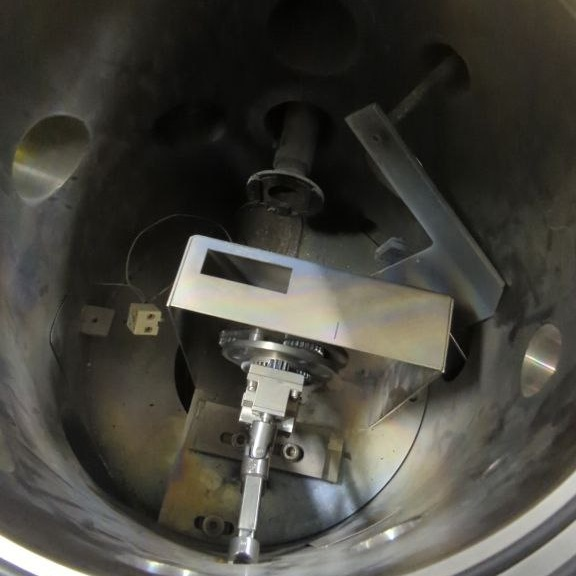
\includegraphics[width=\textwidth]{../assets/messmethoden/heiz/chamber}
        \caption{Innenansicht der Vakuumkammer.}
        \label{fig:vakuumkammer}
    \end{subfigure}
    \begin{subfigure}{0.35\textwidth}
        \centering
        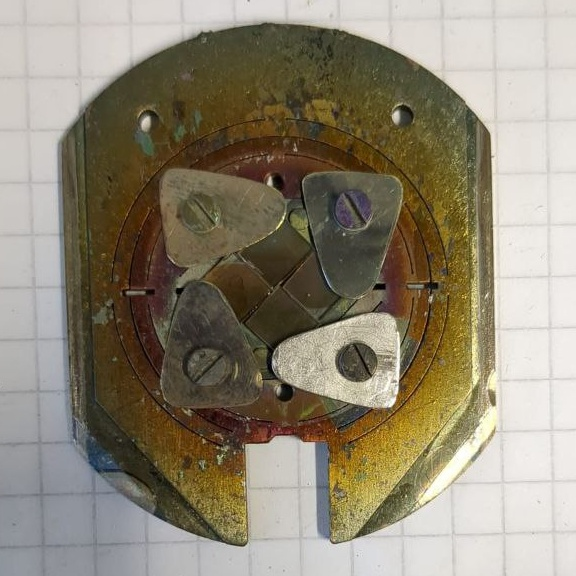
\includegraphics[width=\textwidth]{../assets/messmethoden/heiz/sample_holder}
        \caption{Substrathalter mit montierter Probe.}
        \label{fig:sample_holder}
    \end{subfigure}
    \caption{Für die Ausheizprozesse verwendete Vakuumkammer und verwendeter Substrathalter.}
\end{figure}
Eine für diese Arbeit verwendete Anlage zum Ausheizen der Dünnfilme ist eine Vakuumkammer, die mit einer Möglichkeit
zur Sauerstoffzufuhr ausgestattet ist, siehe \cref{fig:vakuumkammer}.
Die Kammer verfügt über eine Turbomolekularpumpe und eine Vorvakuumpumpe, die zusammen ein Vakuum von bis zu
\qty{e-4}{\milli\bar} erzeugen.
Die Proben werden auf einem Substrathalter, siehe \cref{fig:sample_holder}, montiert und in die Kammer eingesetzt.
Ein Heizlaser ist auf die Rückseite des Substrathalters gerichtet, und die Temperatur der Rückseite des Substrathalters
wird mittels eines Pyrometers gemessen.
Ein PID-Regler steuert die Temperatur, indem er die Laserleistung auf Basis der Temperaturmessungen anpasst, um eine
gleichmäßige Temperatur während des Ausheizprozesses zu gewährleisten.

\paragraph{Muffelofen}
\begin{figure}
    \centering
    \begin{subfigure}[t]{0.35\textwidth}
        \centering
        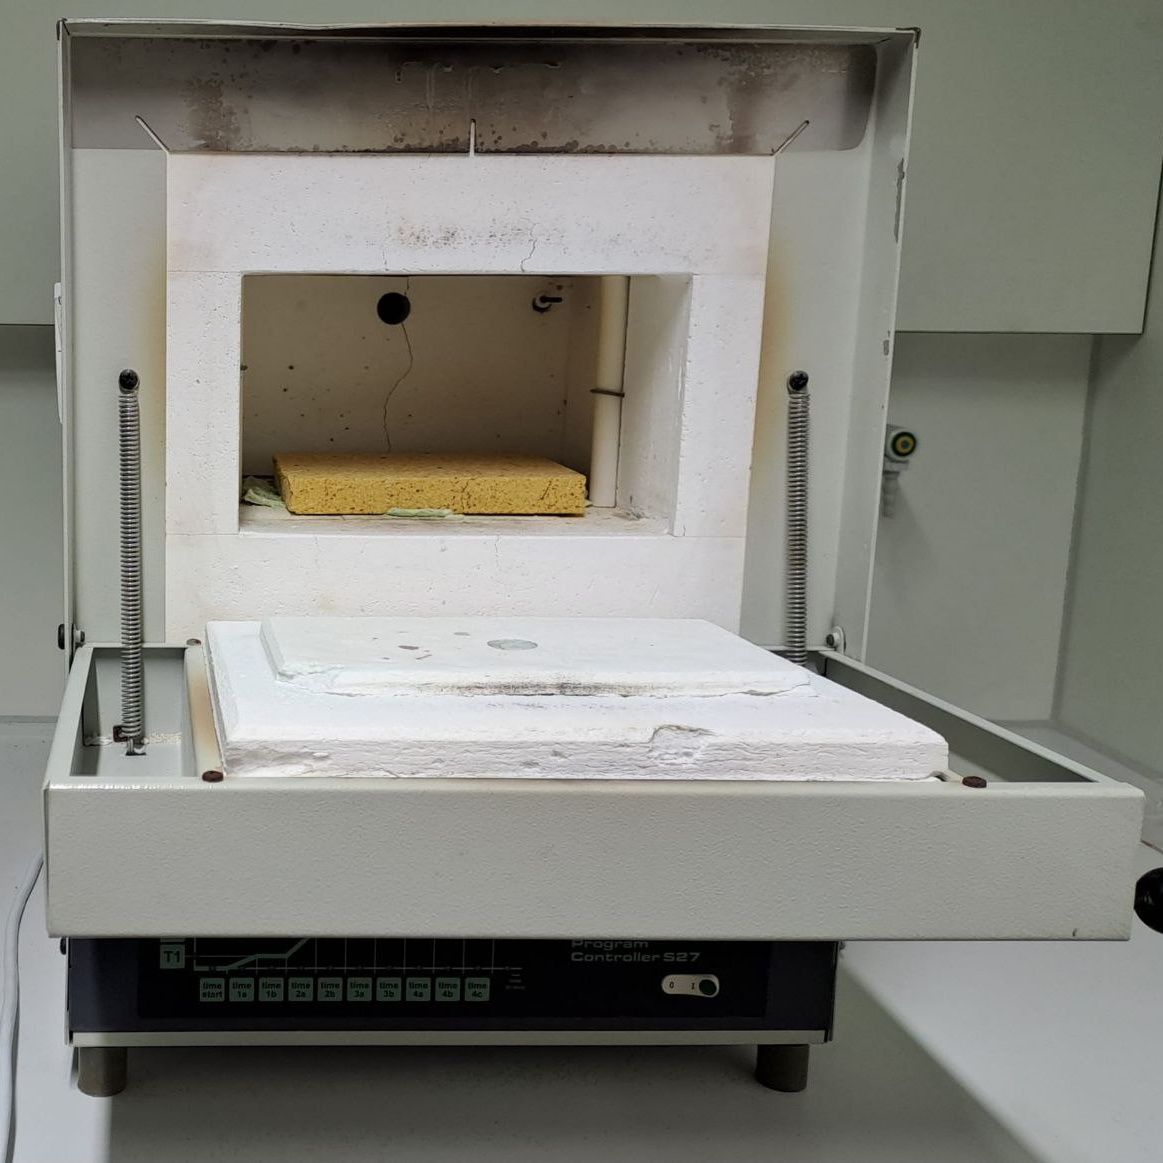
\includegraphics[width=\textwidth]{../assets/messmethoden/heiz/ofen}
        \caption{Innenansicht des Muffelofens.}
        \label{fig:muffelofen}
    \end{subfigure}
    \begin{subfigure}[t]{0.35\textwidth}
        \centering
        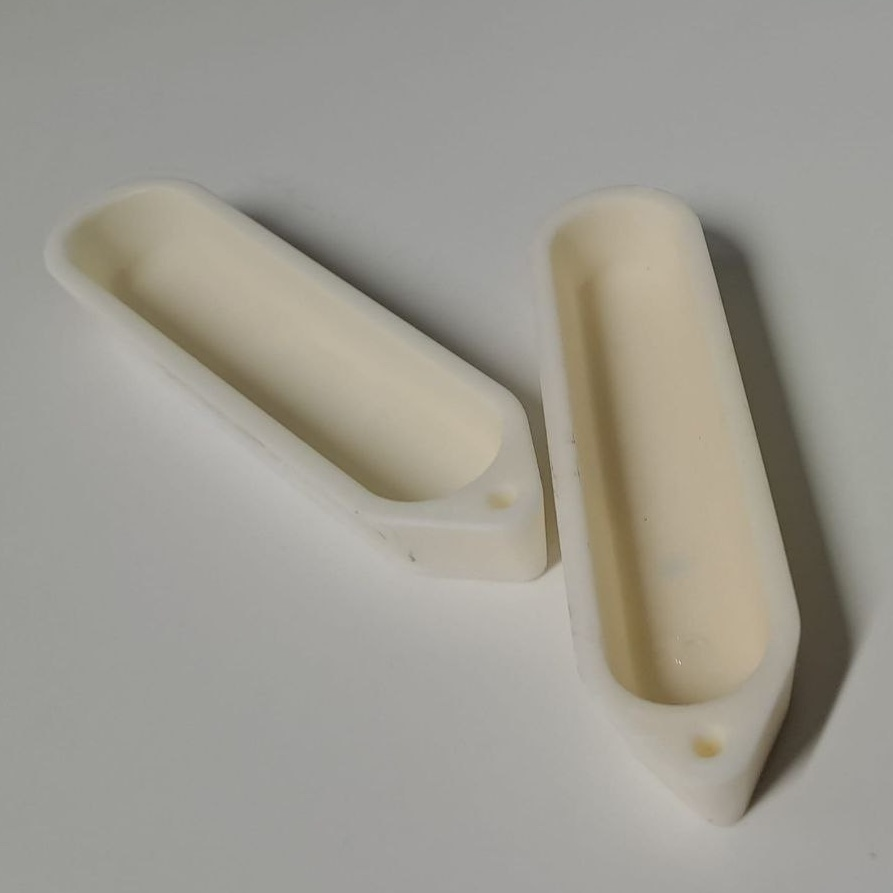
\includegraphics[width=\textwidth]{../assets/messmethoden/heiz/schale}
        \caption{Keramikschalen, in welcher die Proben platziert werden.}
        \label{fig:schale}
    \end{subfigure}
    \caption{Für die Ausheizprozesse verwendeter Muffelofen und Keramikschalen.}
\end{figure}
Neben der Vakuumkammer wurde ein Muffelofen für das Ausheizen der Dünnfilme in einer Luftatmosphäre genutzt,
siehe \cref{fig:muffelofen}.
Der Ofen ist mit einem Temperatursensor ausgestattet, der die Temperatur im Inneren überwacht.
Die Proben werden in einer Keramikschale platziert, siehe \cref{fig:schale}, mit einer zweite
Keramikschale abgedeckt und in den Ofen eingesetzt.

Die Temperaturkontrolle erfolgt auch hier über einen PID-Regler, der die Heizelemente des Ofens reguliert, um
die eingestellte Temperatur konstant zu halten.
Die Proben werden für eine festgelegte Dauer im Ofen belassen, um die gewünschten thermischen Effekte zu erzielen.

\subsection{Röntgendiffraktometrie}\label{subsec:xrd}
Röntgendiffraktometrie (XRD, engl. \textit{X-Ray diffraction}) ist eine weit verbreitete Methode, um die
Kristallstruktur von Dünnfilmen zu bestimmen.
Dabei wird ein Röntgendiffraktometer verwendet.
Im Folgenden wird der Aufbau und die Funktionsweise dieses Gerätes erläutert.
Dabei wird sich an den Erkenntnissen aus \citeauthoryear{btb-xrd} \autocite{btb-xrd} orientiert.

\subsubsection{Röntgendiffraktometer}

\begin{figure}
    \centering
    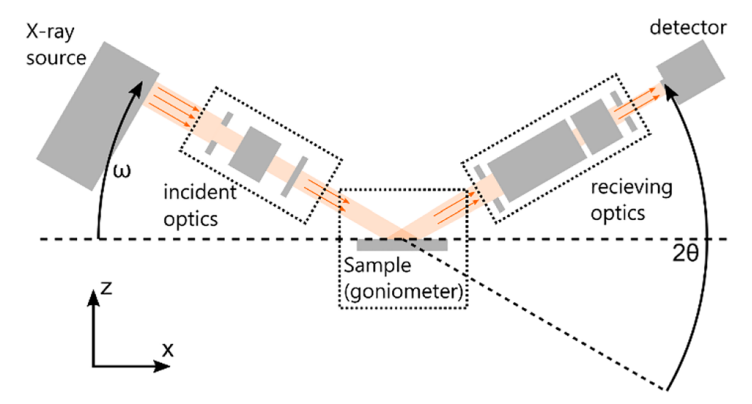
\includegraphics[width=0.6\textwidth]{../assets/messmethoden/xrd/img}
    \caption{Aufbau eines Röntgendiffraktometers. \imcite{btb-xrd}}
    \label{fig:xrd}
\end{figure}

Das Röntgendiffraktometer besteht aus fünf Hauptkomponenten: Röntgenquelle und Detektor, Ein- und Ausfallsoptik,
sowie dem Goniometer.
Zusätzlich ist das Diffraktometer durch eine Strahlungsschutzverkleidung abgeschirmt und mit einer Steuerungssoftware
verbunden.
Ein schematischer Aufbau ist in \cref{fig:xrd} zu erkennen.
Im Folgenden werden die einzelnen Komponenten näher erläutert.

\paragraph{Röntgenquelle}
Die Röntgenstrahlen werden in einer Röntgenröhre erzeugt.
In dieser werden Elektronen aus einer Wolfram-Glühkathode emittiert und durch das elektrische Feld auf eine Anode
beschleunigt.
Die Anode besteht meist aus hochreinem Kupfer.
Stromstärke und Beschleunigungsspannung der Röntgenröhre müssen so gewählt werden, dass die Energie beim Auftreffen der
Elektronen auf die Anode ausreicht, um die gebundenen Elektronen der Atome auf das nächsthöhere Energieniveau anzuregen.
Aufgrund der daraus resultierende Wärme muss die Anode ständig wassergekühlt werden.
Röntgendiffraktometer wird eine Beschleunigungsspannung von \qty{40}{\kilo\volt} und eine Stromstärke
von \qty{40}{\milli\ampere} verwendet.

Nach der Kollision zwischen Kupferatom und Elektron relaxiert das Elektron unter Bildung eines Röntgenphotons.
Man erhält ein Spektrum, welches durch die charakteristische Strahlung der Anode sowie durch Bremsstrahlung
geprägt ist.
Die charakteristische Strahlung wird vorrangig durch die K-Linien, insbesondere $K_{\alpha_1}$, $K_{\alpha_2}$
und K$_{\beta}$, dominiert.
Da $K_{\alpha_1}$ und $K_{\alpha_2}$ energetisch sehr nahe beieinander liegen, können sie nicht immer einzeln
aufgelöst werden.
Die $K_{\beta}$ Strahlung ist größtenteils unerwünscht und kann durch geeignete Filter unterdrückt werden.

Die Wolfram-Glühkathode emittiert unerwünschterweise nicht nur Elektronen, sondern auch Wolfram-Atome in kleinen Mengen.
Über längere Zeiträume führt dies zu einer nicht mehr zu vernachlässigenden Kontamination der Anode.
Dadurch können bei Elektronenstößen auch Wolfram-Atome angeregt werden, was zu einer zusätzlichen Wellenlänge im
Spektrum führt.
In den späteren Messergebnissen sind diese Beiträge erkennbar.
Abschließend gelangen die Röntgenstrahlen durch ein Berylliumfenster in die Einfallsoptik.

\paragraph{Goniometer}
Das Goniometer ist die mechanische Komponente des Röntgendiffraktometers.
Es besteht aus mehreren Drehachsen, die es ermöglichen, die Probe in unterschiedlichsten Winkeln auszurichten.
Nach der Braggschen Beugungstheorie ergeben sich konstruktive Interferenzen an denjenigen Winkeln, die der
Bragg-Bedingung genügen.
Existieren Möglichkeit, die Winkel für Quelle und Detektor zu variieren, kann diese Interferenz beobachtet werden.
Im Allgemeinen ist die Röntgenquelle jedoch fest, eine äquivalente Drehung von Probe und Detektor ist deshalb gängig.
In der einfachsten Betrachtungsweise muss das Goniometer also den Winkel zwischen Probe und Quelle ($\omega$) und dem
Winkel zwischen Probe und Detektor ($2\theta$) einstellen können.
Diese Freiheit reicht zwar für Pulverproben, jedoch nicht für Dünnfilme.
Zwar kann man mit beiden Freiheitsgraden Messungen durchführen, welche die out-of-plane Orientierung charakterisieren,
jedoch ist es nicht möglich, die in-plane Orientierung zu bestimmen.
Dafür werden weitere Achsen, wie $\varphi$ und $\chi$, benötigt.
Eine Konstruktion mit den vier Achsen wird Euler-Wiege genannt.

\paragraph{Ein- und Ausfallsoptik}
Es existieren zwei primäre Möglichkeiten, um den Strahlengang zwischen Quelle, Probe und Detektor zu modifizieren:
Bragg-Brentano-Geometrie und parallele Geometrie.
In der Bragg-Brentano-Geometrie wird ein hochintensiver, divergierender Röntgenstrahl auf die Probe gerichtet,
welcher unter Ausnutzung bestimmter Geometrien zurück auf den Detektor fokussiert werden kann.
Aufgrund der Divergenz des Strahls ist diese Methode fehleranfällig und gerade für $\varphi$ und $\omega$ scans
ist eine Parallelstrahloptik von Vorteil.

Die aus der Quelle austretenden divergierenden Strahlen werden durch einen Göbel-Spiegel
parallelisiert und durchlaufen anschließend einen Eingangs- und Axialspalt, die den Winkelbereich
festlegen.
Dazwischen liegt ein Soller Spalt, der die Divergenz in axialer Richtung begrenzt, da diese
nicht durch den Göbel-Spiegel eliminiert werden kann.
Anschließend reflektiert der Strahl an der Probe und gelangt über weitere Spalte zum Detektor.

\paragraph{Detektor}
Der Röntgendetektor dient dazu, die Intensität der reflektierten Röntgenstrahlen zu messen und
in elektrische Signale umzuwandeln.
Im für die Arbeit verwendeten Röntgendiffraktometer wird ein Halbleiterdetektor verwendet.
Die Grundidee eines Halbleiterdetektors ist, das Material durch Photonen zu ionisieren und dabei freie Ladungsträger zu
erzeugen.
Diese werden über ein elektrisches Feld extrahiert und elektronisch gezählt.
Durch die matrixartige Anordnung einzelner Halbleiterzellen kann die Intensität in Abhängigkeit der Position bestimmt
werden.
Somit können unterschiedliche Detektormodi realisiert werden, wie 0D Punktdetektion,
1D Linien- oder 2D Flächendetektion.
Wichtig ist, dass die maximale Zählrate des Detektors nicht überschritten wird.
Das führt zu nichtlinearen Antworten und kann den Sensor beschädigen.
Um das zu vermeiden, können Filter und Attenuatoren verwendet werden.

\subsubsection{Scanmethoden}
Durch den hohen Freiheitsgrad des Goniometers können unterschiedliche Scanmethoden realisiert werden.
Diejenigen, die in dieser Arbeit verwendet wurden, sind im Folgenden beschrieben.

\paragraph{$2\theta/\omega$ scan}
Ein $2\theta/\omega$ scan ist eine einfache Methode, um die Kristallstruktur von Dünnfilmen zu bestimmen
und bildet die Grundlage für weitere Messungen.
Die Probe wird auf den Probenhalter montiert und in das Goniometer eingesetzt.
Der Winkel zwischen Probenoberfläche und Quelle wird als $\omega$ und der Winkel zwischen Probenoberfläche und Detektor
als $2\theta$ bezeichnet.
Als Anfangsbedingung legt man Messdauer und ein Intervall für $\omega$ fest und startet die Messung.
Nun fahren Goniometer und Detektor über den angegebenen Winkelbereich mit der Bedingung $\omega = \theta$.
Als Ausgabe bekommt man ein Intensitätsprofil in Abhängigkeit von $2\theta$, in denen im Idealfall charakteristische
Peaks erkennbar sind.
Diese Peaks entstammen der Bragg-Reflexion von Kristallebenen, die parallel zur Probenoberfläche liegen.
Kennt man die Wellenlänge der Röntgenstrahlung, so kann man mithilfe des Peaks den Gitterabstand bestimmen.
Somit ist es möglich, Rückschlüsse auf die vorhandenen Kristallstrukturen im Dünnfilm zu ziehen.

\subsection{Rasterkraftmikroskopie}\label{subsec:afm}
Mithilfe der Rasterkraftmikroskopie (AFM, engl. \textit{Atomic Force Microscopy}) kann die Oberflächenstruktur der
Dünnfilme charakterisiert werden.
Das Rasterkraftmikroskop ist ein hochpräzises Messinstrument zum Erfassen von Oberflächenstrukturen.
Anders als bei Licht- oder Elektronenmikroskopie wird hierbei eine mechanische Funktionsweise verwendet.
Dabei fährt der Cantilever, eine Messnadel, rasterweise über eine Oberfläche und tastet diese ab.
Die Spitze des Cantilevers ist im Nanometerbereich dimensioniert und kann so auch kleinste Strukturen erfassen.
Die auf den Cantilever wirkenden interatomaren oder magnetischen Kräfte führen zu messbaren Auslenkungen,
woraus eine Topographiekarte der Oberfläche erstellt wird.
Das in der Arbeit benutzte Rasterkraftmikroskop ist das \textit{XE-150} von Park Systems.
In den folgenden Abschnitten wird der Aufbau und die Funktionsweise des Rasterkraftmikroskops
erläutert, basierend auf den Erkenntnissen von \citeauthoryear{afm-buch} \autocite{afm-buch}.

\subsubsection{Schematischer Aufbau und Funktionsweise}
\begin{figure}
    \centering
    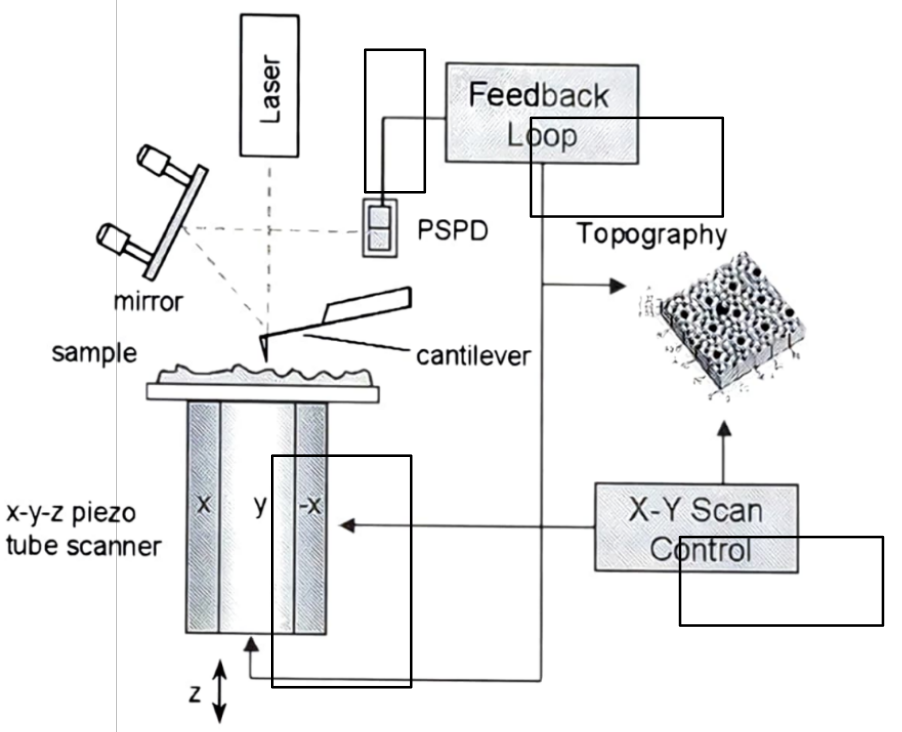
\includegraphics[width=0.6\textwidth]{../assets/messmethoden/afm/01_aufbau}
    \caption{Schematischer Aufbau eines Rasterkraftmikroskops. \imcite{afm-buch}}
    \label{fig:afm_aufbau}
\end{figure}
Die grundlegende Funktionsweise ist in \cref{fig:afm_aufbau} dargestellt.
Fährt der Cantilever über die Probe, so wirken interatomare Kräfte auf die Spitze, welche den Cantilever auslenken.
Diese Auslenkung wird mithilfe eines Laserstrahls und eines Photodetektors gemessen und an ein Feedback System
übergeben.
Basierend auf dem gewählten Betriebsmodus wird entweder versucht, die Auslenkung oder die Schwingungsamplitude
des Cantilevers konstant zu halten.
Mithilfe dieser Regulation wird ein Korrektursignal ausgegeben, welches die Position des Cantilevers anpasst.
Dies geschieht mithilfe von Piezoelementen, wodurch der Cantilever in $\mathrm{z}$-Richtung und die Probe in
$\mathrm{x}$- und
$\mathrm{y}$-Richtung bewegt werden kann.
Die z-Position des Cantilevers wird aufgezeichnet und als Topographiesignal am Computer ausgewertet.
Im Folgenden werden die einzelnen Komponenten näher erläutert.

\paragraph{Auslenkungserkennungssystem}
\begin{figure}
    \centering
    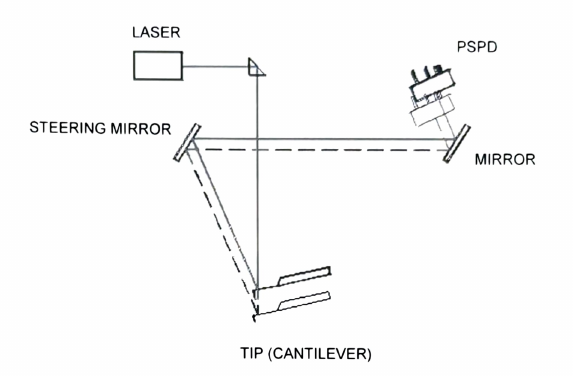
\includegraphics[width=0.6\textwidth]{../assets/messmethoden/afm/02_beam}
    \caption{Schematischer Aufbau eines Auslenkungserkennungssystems. \imcite{afm-handbuch}}
    \label{fig:afm-beam}
\end{figure}
Das System zur Auslenkungserkennung ist in \cref{fig:afm-beam} dargestellt.
Ein Laserstrahl wird aus einer Laserdiode emittiert und auf die Rückseite des Cantilevers gerichtet.
Dieser besitzt eine reflektierende Rückseite, sodass der Strahl am Cantilever zum beweglichen Spiegel reflektiert wird.
Über diesen lässt sich die Position des Strahls auf den Photodektor einstellen.
Der Strahl wird durch einen letzten Spiegel auf den Photodetektor reflektiert.


Der Photodetektor besteht aus vier Segmenten, welche in einem Quadrat angeordnet sind, wobei jedes Segment einen
Quadranten dieses Quadrats belegt.
Damit kann die Intensität des reflektierten Strahls ortsaufgelöst gemessen werden.
Im unausgelenkten Zustand muss der bewegliche Spiegel so eingestellt werden, dass der Strahl mittig auf die vier
Segmente trifft.
Kommt es zur Auslenkung, ändert sich der Winkel des Cantilevers und damit auch die Position des Strahls auf dem
Photodetektor.
Über die vier Segmente können Auslenkung und Torsion des Cantilevers bestimmt werden.

\paragraph{Feedback Controller}
Damit eine genaue Topografiekarte aufgezeichnet werden kann, ist ein schnelles und präzises Regelsystem nötig.
Durch die Regelung soll eine vorgegebene Kenngröße, beispielsweise die Auslenkung des Cantilevers, möglich konstant
gehalten werden.
Für diesen Zweck wird ein geschlossenes Regelkreissystem verwendet.
Der Regler besteht aus einem Proportional-Integral-Controller (PI-Controller), der das Fehlersignal zwischen dem
gemessenen Wert und dem Sollwert verarbeitet.
Der Proportionalanteil reagiert direkt auf den aktuellen Fehler, während der Integralanteil konstante Störungen über
die Zeit eliminiert.
Die Kombination beider Anteile ermöglicht es, sowohl kurzzeitige als auch langzeitige Abweichungen zu
korrigieren.

\paragraph{Positionierung}
Piezoelemente werden verwendet, um den Cantilever in $\mathrm{z}$-Richtung und die Probe in $\mathrm{xy}$-Richtung zu
bewegen, basierend auf dem Piezoeffekt.
Dieser Effekt tritt auf, wenn bestimmte Kristalle wie Quarz unter mechanischer Spannung elektrische Spannung erzeugen
können.
Durch Anlegen einer elektrischen Spannung an Piezokristalle können Deformationen im Bereich von \qty{0.1}{\nano\meter}
und damit in atomaren Dimensionen erreicht werden.
Spezielle Metallbiegeelemente mit eingebetteten Piezoelementen ermöglichen gezielte Verformungen, um Bewegungen
in verschiedenen Richtungen zu erzeugen.
Damit kann sowohl die Probe in $\mathrm{xy}$-Richtung, als auch der Cantilever in $\mathrm{z}$-Richtung bewegt werden.
Die Feinpositionierung und Scanbewegungen in der Rasterkraftmikroskopie werden durch Piezo-Biegeelemente gesteuert,
während eine Grobpositionsbühne für die grobe Positionierung verwendet wird.

\subsubsection{Interaktion zwischen Probe und Spitze}
Die auf die Spitze wirkende Gesamtkraft setzt sich aus verschiedenen Komponenten zusammen.
Der wichtigste und weitreichendste Beitrag entspringt der Van-der-Waals Wechselwirkung, einer attraktiven Kraft,
die durch die spontane Ausbildung fluktuierender Dipole entsteht.
Für kleinere Distanzen müssen zwei weitere Interaktionen berücksichtigt werden.
Überlappen die äußeren Elektronenhüllen von Proben- und Spitzenatomen, so können chemische Bindungen entstehen, welche
attraktive oder repulsive Kräfte hervorrufen.
Für noch kleinere Distanzen wird die Pauli-Abstoßung zwischen den Elektronen der Atome relevant.
Da die geschlossenen Elektronenschalen der Atome nicht überlappen können, müssen die zusätzlichen Elektronen auf ein
höheres Energieniveau gehoben werden.
Dadurch entsteht eine effektive repulsive Kraft.

Obwohl das System quantenmechanisch präzise beschrieben werden kann, ist die Lösung solch komplexer Systeme
nicht trivial.
Aus diesem Grund werden Modellpotentiale genutzt, die die Interaktionen zwischen Probe und Spitze approximieren.
Ein beliebtes ist das Lennard-Jones-Potential, welches sowohl die Van-der-Waals Wechselwirkung als auch die repulsiven
Anteile berücksichtigt:
\begin{equation}
    U_{\mathrm{LJ}}=4U_{0}\left[ \left( \frac{R_{\mathrm{a}}}{r} \right)^{12} -\left( \frac{R_{\mathrm{a}}}{r}
    \right)^{6}\right].
    \label{eq:lennard_jones}
\end{equation}
Hierbei ist $U_{0}$ die Tiefe des Potentials, $R_{\mathrm{a}}$ der Gleichgewichtsabstand und $r$ der Abstand zwischen
den Atomen.
Das Potential ist in \cref{fig:lennard_jones} dargestellt.
Auch wenn das Lennard-Jones-Potential für interatomare Wechselwirkungen entwickelt wurde, erklärt es die relevanten
Kräfte zwischen Probe und Spitze.

\begin{figure}
    \centering
    \import{../plots/messmethoden/}{lennard_jones_potential.pgf}
    \caption{Lennard-Jones-Potential.}
    \label{fig:lennard_jones}
\end{figure}

\subsubsection{Betriebsmodi}
Das Rasterkraftmikroskop verfügt über unterschiedliche Betriebsmodi.
In der vorliegenden Arbeit wurde der statische Kontaktmodus verwendet, um die Oberflächenstruktur zu erfassen.
Dabei wird die Probe in $\mathrm{xy}$-Richtung bewegt, während die Spitze des Cantilevers einen so kleinen Abstand zur
Probe hat, dass die repulsiven Kräfte dominieren.
Für den statischen Kontaktmodus liegt der Abstand im Definitionsbereich der orange dargestellten Kurve in
\cref{fig:lennard_jones}.
In diesem Bereich ist die Ableitung des Potentials negativ, was zu einer repulsiven Kraft führt.
Diese bewirkt eine Auslenkung $\Delta z$ des Cantilevers, welche durch das Erkennungssystem aufgezeichnet wird.
Mithilfe eines \textit{setpoint}-Parameters wird eine konstante Auslenkung festgelegt, die vom Feedback-System
eingehalten wird.
Scannt man über eine Erhöhung, so ändert sich die Auslenkung und das Feedback-System versucht, den Cantilever erneut
auszurichten, indem es die Höhe anpasst.
Dadurch entsteht eine Topografiekarte der Oberfläche.
Da sich die Spitze in stetigem Kontakt mit der Oberfläche befindet, müssen die Wechselwirkungskräfte
möglichst klein gehalten werden, da ansonsten die Spitze leicht kontaminiert oder beschädigt werden kann.

Nicht nur statische, sondern auch dynamische Betriebsmodi existieren.
Dabei wird der Cantilever mit einer bestimmten Frequenz und Amplitude angeregt, während er über die Probe fährt.
Ändert sich die Kraft, dann ändert sich die Resonanzfrequenz und damit auch die Amplitude.
Das Topografiesignal wird durch die Forderung einer konstanten Amplitude erzeugt.

Die in der Arbeit aufgenommenen AFM-Bilder wurden stets mit einer Scanrate von \qty{1}{\hertz}, einem
Setpoint von \num{0.4} und, bis auf eine Ausnahme, einem Scanbereich von $\qty{5}{\micro\meter} \times
\qty{5}{\micro\meter}$ aufgenommen.
Für alle Aufnahmen wurden NSC18-TI/PT Cantilever von MikroMasch verwendet.

\subsection{Weitere Messmethoden}\label{subsec:weitere-messmethoden}
Die in diesem Abschnitt vorgestellten Methoden wurden für die Arbeit verwendet, werden aber
nicht im Detail erläutert.

\paragraph{Profilometer}
Ein Profilometer ist ein Messinstrument, welches zur präzisen Messung von Oberflächenprofilen verwendet wird.
Sowohl die Topografie als auch die Rauheit der Oberfläche können hiermit bestimmt werden.
Im Gegensatz zum Rasterkraftmikroskop ist das Profilometer für gröbere Oberflächenstrukturen auf größeren Flächenskalen
ausgelegt.
Das verwendete Profilometer \textit{DektakXT} von Bruker fährt mit einer Diamantspitze über die Probe, um
die Oberflächenstruktur zu erfassen.

Die mithilfe von PLD hergestellten Dünnfilme sind durch Klemmen an den Substrathalter montiert, welche
üblicherweise kleine Regionen des Substrats, meist die Ecken, verdecken.
Da an diesen Stellen kein Dünnfilm abgeschieden wird, kann mithilfe dieser Regionen die Dicke des
Dünnfilms bestimmt werden, indem die Spitze des Profilometers sowohl über Dünnfilm als auch über eine
verdeckte Stelle fährt.
Der Höhenunterschied zwischen beiden Stellen entspricht der Dicke des Dünnfilms.

\paragraph{Energiedispersive Röntgenspektroskopie}
Eine weitere wichtige Methode zur Charakterisierung von Dünnfilmen ist die energiedispersive Röntgenspektroskopie
(EDX, engl. \textit{energy dispersive X-ray spectroscopy}), welche ortsaufgelöste chemische Kompositionsanalysen
ermöglicht.
Hierbei werden die Atome des Dünnfilms durch den Elektronenstrahl eines Rasterelektronenmikroskops (SEM, engl.
\textit{scanning electron microscope}) angeregt, welcher durch Stoßprozesse innere Elektronen aus den Atomen
herausschlägt.
Durch die anschließende Relaxation werden Röntgenstrahlen emittiert, deren Energie charakteristisch für das jeweilige
Element ist.
Die Energien der Röntgenstrahlen werden mithilfe eines Detektors aufgezeichnet und in ein Spektrum umgewandelt, welches
die Intensität in Abhängigkeit der Energie darstellt.
Da mehrere Elektronenübergänge bei der Relaxation möglich sind, entstehen in diesem Spektrum mehrere charakteristische
Peaks pro Element.
Durch die Position der Peaks können die enthaltenen Elemente ermittelt werden,
die korrespondierende Intensität gibt Aufschluss über die Konzentration der Elemente \autocite{edx}.




    %\section{Auswertung}\label{sec:auswertung}
Von Jorrit Bredow wurden vier Proben \samplethree, \sampleone, \sampletwo, \samplefour\ in vier Prozessen einer
PLD-Anlage mit $\qty{10}{\milli\meter} \times \qty{10}{\milli\meter}$ Eagle XG Glassubstraten und dem in
\cref{subsec:pld} beschriebenen Target hergestellt.
Für jeden Prozess wurden jeweils \num{20000} Laserpulse mit einer Frequenz von \qty{20}{\hertz} und einer Energie von
\qty{650}{\milli\joule} abgegeben.
Dabei wurde der eingebaute Widerstandsheizer nicht verwendet.
Der variable Parameter war der Abscheidedruck der Sauerstoffatmosphäre innerhalb der Kammer.
Nach der Herstellung wurden die Proben im Profilometer und im Röntgendiffraktometer bezüglich ihrer Schichtdicke
vermessen.
Der jeweilige Druck und die Schichtdicken sind in \cref{tab:samples} aufgeführt.
\begin{table}[h]
    \centering
    \begin{tabular}{l l l l l}
        \toprule
        Probenname & \makecell[l]{Abscheidedruck \\ in \unit{\milli \bar}} & \makecell[l]{Dicke in \unit{\nano\meter} \\
        Profilometermessung} & \makecell[l]{Dicke in \unit{\nano\meter}     \\ XRR Messung}   \\
        \midrule
        \samplethree   & \num{0.1}   & \num{65(4)} & \num{109} \\
        \sampleone  & \num{0.01} & \num{95(7)} & - \\
        \sampletwo  & \num{0.001} & \num{160(12)} & \num{142} \\
        \samplefour  & \num{0.00005} & \num{135(16)} & \num{120} \\
        \bottomrule
    \end{tabular}
    \caption{Abscheidedruck und Schichtdicken der zu untersuchenden Proben}
    \label{tab:samples}
\end{table}

In jedem Prozess ist neben dem Eagle XG Glassubstrat ein c-Saphir Substrat eingebaut worden.
Damit konnten vier weitere Proben \csamplethree, \csampleone, \csampletwo, \csamplefour\ hergestellt werden, welche
jedoch ausschließlich für die Konzentrationsanalyse von \cref{subsec:edx-analyse} Verwendung finden.
Der untere Index der Bezeichnung steht erneut für den Abscheidedruck in \unit{\milli \bar}.

Im Anschluss an die Probenherstellung wurden \samplethree, \sampleone, \sampletwo, \samplefour\ in
$\qty{5}{\milli\meter}\times \qty{5}{\milli\meter}$ gevierteilt, damit Ausheizstudien mit unterschiedlichen Atmosphären
vergleichbar durchgeführt werden konnten.
Dazu wurde der Dünnfilm der jeweiligen Probe mit Photolack beschichtet, um die Oberfläche vor
mechanischen Beschädigungen beim Zersägen zu schützen.
Das Substrat wurde mit der Dünnfilmseite nach oben auf eine Glasplatte mit Wachs geklebt und mit einer
Diamantsäge zerteilt.
Anschließend wurden Wachs und Photolack mit Wachsentferner, NMP und Ethanol entfernt.
Es ist zu beachten, dass diese Prozedur durch die Lösungsmittel die Zusammensetzung und Oberfläche des Dünnfilms
verändern kann.
Optisch wurden keine Veränderungen festgestellt.

Nach der Präparation wurden die Eagle XG Proben auf drei verschiedene Arten ausgeheizt:
In der im \cref{subsec:ausheiz} vorgestellten Vakuumkammer unter Sauerstoffatmosphäre, in der Vakuumkammer unter
Vakuumbedingungen und im Muffelofen aus \cref{subsec:ausheiz} unter Luftatmosphäre.

Um einen Ausgangspunkt für die Temperatur festzulegen, wurde sich an den Erkenntnissen von Rost (2015) orientiert.
In diesem Paper wurden, wie in \cref{subsubsec:heo} beschrieben, Pellets angefangen bei \qty{750}{\degreeCelsius}
auszuheizen.
Bei dieser Temperatur wurden mehrere Phasen beobachtet, ausgeprägte Peaks der Natriumchloridstruktur waren jedoch
bereits erkennbar \autocite{Rost2015}.
Da sich Dünnfilme nicht wie massive Proben verhalten, wurde die Temperatur auf \qty{600}{\degreeCelsius} festgelegt,
um sicherzustellen, dass die Phasenübergangstemperatur nicht zu Beginn bereits überschritten wird.
Um dies zu überprüfen, wurde eine der vier geviertelten Proben von \sampletwo\ in Luft auf \qty{600}{\degreeCelsius}
für eine Stunde ausgeheizt und anschließend im Röntgendiffraktometer vermessen.
Da keine Peaks des Dünnfilms zu erkennen waren, wurde diese Probe anschließend für drei Stunden und sonst identischen
Bedingungen auf \qty{600}{\degreeCelsius} ausgeheizt und erneut im Röntgendiffraktometer vermessen.
Auch hier waren keine Peaks des Dünnfilms zu erkennen, weshalb die Temperatur als Ausgangspunkt für den
Sauerstoff-Ausheizvorgang festgelegt wurde.

Während des Sauerstoffausheizvorgangs wurde ein nichtsignifikanter Peak bei ${2\theta}{\approx}\qty{30}{\degree}$
ab einer Temperatur von \qty{600}{\degreeCelsius} beobachtet, welcher ein Hinweis auf eine Phasenbildung sein könnte.
% TODO nachgucken
Aus diesem Grund wurde beim Vakuumausheizvorgang die Starttemperatur auf \qty{500}{\degreeCelsius} festgelegt.
Da keine signifikanten Peaks in dieser Serie zu erkennen waren, wurde die Starttemperatur erneut
auf \qty{600}{\degreeCelsius} für die Ausheizung im Muffelofen gesetzt.

Da die Dünnfilme auf Eagle XG Glassubstraten gewachsen sind, muss die Viskosität des Glases in Abhängigkeit der
Temperatur beachtet werden.
Der obere Kühlpunkt des Glases liegt bei \qty{722}{\degreeCelsius}.
Bis zu diesem Punkt treten zwar Entspannungen auf, Formänderungen sind jedoch nicht zu erwarten.
Der Erweichungspunkt des Glases liegt bei \qty{971}{\degreeCelsius}.
Ab dieser Temperatur beginnt das Glas merklich zu fließen und sich unter Einfluss des Eigengewichts zu verformen.
Da die Dünnfilme im Substrathalter der Vakuumkammer unter mechanischer Spannung stehen, ist bereits bei
\qty{875}{\degreeCelsius} eine Deformierung erkennbar, sodass diese Temperatur als obere Grenze für die Ausheizstudien
in der Vakuumkammer festgelegt wurde.
Diese Temperatur ist außerdem die von Rost verwendete Phasenübergangstemperatur für massive äquimolare Proben.
\autocite{Rost2015}
Für den Ausheizvorgang im Muffelofen wurde die Temperatur auf \qty{950}{\degreeCelsius} festgelegt, da diese noch
unterhalb des Erweichungspunkts des Glases liegt.

Für den Sauerstoffausheizvorgang wurde die Vakuumkammer mit einer Sauerstoffatmosphäre von circa \qty{800}{\milli\bar}
verwendet.
Die Proben \samplethree, \sampleone, \sampletwo, \samplefour\ wurden einem Prozess aus wiederholtem Ausheizen und
anschließendem Messen unterzogen.
Als Ausheiztemperaturen sind \qtylist{600;700;750;800;875}{\degreeCelsius} gewählt worden.
Dabei dienen \qty{750}{\degreeCelsius} und \qty{875}{\degreeCelsius} als Referenztemperaturen zur Forschung
von Rost \autocite{Rost2015}.
Die Proben wurden für eine Stunde bei der jeweiligen Temperatur ausgeheizt, vom Substrathalter entfernt und auf eine
Glasplatte gelegt, um ein schnelles Abkühlen zu erreichen.
Während des Ausheizens rotierte der Substrathalter mit einer Winkelgeschwindigkeit von
\qty{1080}{\degree\per\minute}, um eine
gleichmäßige Temperaturverteilung zu gewährleisten.

Für den Ausheizvorgang unter Vakuumbedingungen wurde die gleiche Vakuumkammer wie für den Sauerstoffausheizvorgang
verwendet.
Auch hier wurden die Proben \samplethree, \sampleone, \sampletwo, \samplefour\ einem Prozess von wiederholendem
Ausheizen und anschließendem Messen unterzogen.
Die Kammer wird auf einen Druck von \qty{4e-4}{\milli\bar} evakuiert, um Vakuumbedingungen zu erreichen.
Dies ist die geringste Druckstufe, die der PID-Regler der Vakuumkammer zuverlässig erreicht.
Alle anderen Parameter sind identisch zum Sauerstoffausheizvorgang.

Für den Ausheizvorgang in Luftatmosphäre wurde der Muffelofen verwendet.
Die Proben \samplethree, \sampleone, \sampletwo, \samplefour\ wurden einem Zyklus von Ausheizen und anschließendem
Messen unterzogen.
Für das Ausheizen wurden die Temperaturen \qtylist{600;700;750;800;875;950}{\degreeCelsius} gewählt.
Die Proben wurden in einer Keramikschale für eine Stunde bei der jeweiligen Temperatur ausgeheizt, anschließend
aus dem Ofen und der Schale genommen und auf einer Glasplatte abgekühlt.
Anders als bei den vorherigen Ausheizvorgängen wurde die Probe mit einer langsamen Ausheizrate von
\qty{300}{\kelvin\per\hour} auf die Endtemperatur gebracht.

\subsection{Temperaturkalibrierung der A-Kammer}\label{subsec:temperaturkalibrierung}
\begin{figure}
    \centering
    \foreach \i/\desc in {
        furnace_calibration_1.pgf/{Kalibrierung des Lithografiesensors, Bild 1},
        furnace_calibration_2.pgf/{Kalibrierung des Lithografiesensors, Bild 2},
        a_chamber_calibration.pgf/{Kalibrierung der Vakuumkammer},
        final_calibration.pgf/{Abhängigkeit zwischen $T_{\mathrm{Pyro}}$ und $T_{\mathrm{Lit}}$},
        quenching_time.pgf/{Abkühlzeit der Vakuumkammer}
    }{
        \begin{subfigure}[t]{0.49\textwidth}
            \import{../plots/calibration}{\i}
            \caption{\desc}
            \label{fig:\i}
        \end{subfigure}
    }
    \caption{Abhängigkeiten zur Temperaturbestimmung der Vakuumkammer}
    \label{fig:temperature_calibration_1}
\end{figure}
Zentrales Thema der vorliegenden Arbeit ist das Ausheizen und anschließende Charakterisieren der \heo\ Dünnfilme.
Dafür wird unter anderem die Vakuumkammer aus \cref{subsec:ausheiz} verwendet.
In dieser ist ein Heizlaser verbaut, welcher auf die Rückseite des Substrathalters
gerichtet ist.
Durch ein Pyrometer wird die Temperatur auf der Rückseite des Substrathalters gemessen.
Die relevante Temperatur ist jedoch die des Dünnfilms auf der Vorderseite des Substrathalters, welche durch die
Atmosphäre, die Geometrie und Wärmeleitfähigkeit des Substrathalters und des Substrats beeinflusst wird.

Um diese abzuschätzen, wurde von Tim Düvel ein spezieller Temperatursensor hergestellt.
Dieser besteht aus einem c-Saphir Substrat, auf dem eine Maske für die Platinbahnen infolge eines
Lithografieprozesses aufgebracht wurde.
Das Substrat wurde zunächst für \qty{10}{\second} mit Platinoxid für und anschließend für \qty{120}{\second} mit Platin
im Sputterverfahren beschichtet.
Nach dem Ablösen der Maske wurde das Substrat durch das gleiche Verfahren an beiden Enden der Platinbahnen mit Gold beschichtet.
Zum Schutz der Platinbahnen vor mechanischer Beschädigung wurde eine Schicht Aluminiumoxid aufgebracht.
Dieser Sensor wird im Folgenden als Lithografiesensor bezeichnet.

In Zusammenarbeit mit Tim Düvel wurde eine Kalibrierung des Lithografiesensors durchgeführt.
Dazu wurde ein PT1000-Temperatursensor genutzt, für welchen eine bekannte quadratische Abhängigkeit zwischen Widerstand
$R_{\mathrm{Pt}}$ und Temperatur $T_{\mathrm{Pt}}$ existiert\autocite{din_pt}:
\begin{equation}
    R_{\mathrm{Pt}}(T_{\mathrm{Pt}})
    =R_0 \cdot (1 + A \cdot T_{\mathrm{Pt}} + B \cdot T_{\mathrm{Pt}}^2).
    \label{eq:pt1000_calibration}
\end{equation}
Hierbei ist $R_0 = \qty{1000}{\ohm}$ der Widerstand bei \qty{0}{\degreeCelsius},
$A = \qty{3.9083e-3}{\degreeCelsius^{-1}}$ und $B = \qty{-5.775e-7}{\degreeCelsius^{-2}}$.
Der PT1000-Temperatursensor wurde mithilfe von Wärmeleitpaste thermisch an den Lithografiesensor gekoppelt und
in einem Muffelofen ausgeheizt.
Der Widerstand des Lithografiesensors $R_\mathrm{Lit}$ und der des PT1000-Temperatursensors $R_\mathrm{Pt}$
wurden in Abhängigkeit der Zeit gemessen und sind in Abbildung \cref{fig:furnace_calibration_1.pgf} dargestellt.
Aus der Parametrisierung $t \to (R_\mathrm{Lit}(t), R_\mathrm{Pt}(t))$ kann die Abhängigkeit beider Widerstände
voneinander bestimmt werden.
Aufgrund der gleichen Materialbeschaffenheit ist die Abhängigkeit $R_\mathrm{Lit}(R_\mathrm{Pt})$ linear und kann durch
einen linearen Fit der Form $f(x)=mx+n$ beschrieben werden, siehe \cref{fig:furnace_calibration_2.pgf}.
Für die Fitparameter ergibt sich:
\begin{equation*}
    m = \num{0.501(0.0002)} \quad n = \qty{-0.176(0.001)}{\kilo\ohm}.
\end{equation*}

Im nächsten Schritt wurde der Lithografiesensor in den Probenhalter der Vakuumkammer eingebaut und eine
zweite Messung durchgeführt.
Dabei wird die Temperatur des Heizlasers eingestellt und nach einer festen Zeitspanne die Pyrometertemperatur
$T_\mathrm{Pyro}$ und der Lithografiewiderstand $R_\mathrm{Lit}$ gemessen.
Es wurden zwei separate Messreihen durchgeführt: Eine bei steigender Temperatur und eine bei abfallender Temperatur.
Auch hier zeigt sich eine lineare Abhängigkeit zwischen beiden Größen, dessen Parameter durch einen linearen Fit
ermittelt werden können, siehe \cref{fig:a_chamber_calibration.pgf}.
Für die Fitparameter ergibt sich:
\begin{equation*}
    m = \qty{0.0067(0.0002)}{\kilo\ohm\per\degreeCelsius} \quad n = \qty{2.6(0.1)}{\kilo\ohm}.
\end{equation*}
Als Referenztemperatur, und damit als Temperatur des Dünnfilms, wird die Temperatur des PT1000-Sensors angesehen.
Diese kann durch folgende Gesamtfunktion bestimmt werden:
\begin{equation}
    T_{\mathrm{Pt}}=\underbrace{ T_{\mathrm{Pt}}(R_{\mathrm{Pt}}) }_{
        \substack{\text{quadratische} \\ \text{Abhängigkeit}}}
    =T_{\mathrm{Pt}}(\underbrace{ R_{\mathrm{Pt}}(R_{\mathrm{Lit}}) }_{
        \substack{\text{lineare} \\ \text{Abhängigkeit}}  })
    =T_{\mathrm{Pt}}(R_{\mathrm{Pt}}(\underbrace{ R_{\mathrm{Lit}}(T_{\mathrm{Pyro}}) }_{
        \substack{\text{lineare} \\ \text{Abhängigkeit}}  }))
    \label{eq:temperature_calibration}
\end{equation}
Da alle Funktionen bekannt sind, zeigt sich folgender Zusammenhang zwischen $T_{\mathrm{Pyro}}$ und $T_{\mathrm{Pt}}$
in \cref{fig:final_calibration.pgf}.
Der Graph zeigt, dass die Temperatur des Dünnfilms mit einer Unsicherheit von circa \qtyrange{10}{15}{\degreeCelsius}
der Temperatur des Pyrometers entspricht.

Wichtig für das Ausheizen ist außerdem die Abkühlzeit der Vakuumkammer.
Um diese zu untersuchen, wurde der Lithografiesensor eingebaut und das der Heizlaser auf \qty{350}{\degreeCelsius}
eingestellt.
Nachdem sich ein konstanter Lithografiewiderstand eingestellt hatte, wurde der Heizlaser abgeschaltet und der
Widerstand in Abhängigkeit der Zeit gemessen, siehe \cref{fig:quenching_time.pgf}.
Für einen Temperaturabfall von circa \qty{350}{\degreeCelsius} auf circa \qty{25}{\degreeCelsius}
benötigt die Vakuumkammer etwa \qty{4}{\minute}.
Damit zeigt der Temperaturbereich, die Präzision des Pyrometers und die Abkühlzeit, dass
die Vakuumkammer für die Ausheizstudien geeignet ist.

Es ist zu beachten, dass dieser Sensor bestmöglich die Thermodynamik von c-Saphir Substraten erfasst.
Die in dieser Arbeit betrachteten Dünnfilme wurden auf Eagle XG Glassubstraten abgeschieden.
Eagle XG hat bei Raumtemperatur eine Wärmeleitfähigkeit von \qty{1.09}{\watt\per\meter\per\kelvin}, wohingegen
c-Saphir eine Wärmeleitfähigkeit von \qty{42}{\watt\per\meter\per\kelvin} hat.
Auch bei einer Temperatur von \qty{300}{\degreeCelsius} hat Eagle XG eine Wärmeleitfähigkeit von
\qty{1.34}{\watt\per\meter\per\kelvin}, wohingegen c-Saphir eine Wärmeleitfähigkeit von
\qty{20}{\watt\per\meter\per\kelvin} hat.
Da die Wärmeleitfähigkeit von Eagle XG Glassubstraten um mehr als eine Größenordnung geringer ist als die von
c-Saphir Substraten, ist die Abschätzung der Temperatur des Dünnfilms durch den Lithografiesensor nur als
Approximation zu betrachten.
Würde man das c-Saphir Substrat des Sensors durch ein Eagle XG Glassubstrat ersetzen, würde die gemessene Temperatur
niedriger ausfallen.

\subsection{Konzentrationsanalyse}\label{subsec:edx-analyse}
Die Abscheidung mithilfe von PLD ist ein hochkomplexer Prozess, welcher nicht im thermodynamischen Gleichgewicht
stattfindet und damit schwer analytisch zu beschreiben ist.
Durch die komplexen Wechselwirkungen der Laserpulse mit den sechs verschiedenen Konstituenten des Targets
ist es schwer, Vorhersagen über die Stöchiometrie des Dünnfilms zu treffen.
Die Komposition des Dünnfilms muss nicht der des Targets entsprechen.
Zu diesem Anlass wurden von Jorrit Bredow ortsaufgelöste Konzentrationsaufnahmen der Proben \csamplethree, \csampleone,
\csampletwo, \csamplefour\ mithilfe von SEM-EDX durchgeführt.

Das Dünnfilmwachstum ist nicht nur abhängig von den Prozessparametern, sondern auch vom gewählten Substrat.
Idealerweise sollte die Konzentrationsanalyse demnach auf demselben Substrat durchgeführt werden, welches auch im
Ausheizprozess verwendet wurde.
Problematisch ist, dass die genaue Zusammensetzung des Eagle XG Glassubstrats nicht bekannt ist.
Es ist jedoch bekannt, dass Magnesium ein Konstituent des Substrats ist.
Da auch der Dünnfilm Magnesium enthält, ist es dadurch nicht möglich, das Magnesium des Dünnfilms vom Magnesium des
Substrats zu unterscheiden.
Daher wurde ein c-Saphir Substrat verwendet, welches keine Metallkationen des Dünnfilms enthält.

Da SEM-EDX Messungen nur auf leitenden Proben durchgeführt werden können und die Dünnfilmee isolierende Eigenschaften
aufweisen, wurden die c-Saphir Proben vor der Messung mit einer dünnen Schicht Kohlenstoff beschichtet.
\cref{fig:edx_map} zeigt die Oberfläche der Probe \csamplethree\ unter der Kohlenstoffschicht.
Erkennbar ist eine glatte Morphologie ohne sichtbare Verunreinigungen.
Die \cref{fig:edx_Mg,fig:edx_Co,fig:edx_Ni,fig:edx_Cu,fig:edx_Zn} zeigen die Konzentrationen der
Elemente Magnesium, Cobalt, Nickel, Kupfer und Zink in Abhängigkeit der Position.
Über den gesamten Dünnfilm ist eine gleichmäßige Verteilung alle Elemente erkennbar.
Es breiten sich keine erkennbaren Cluster aus, welche auf eine Phasentrennung hindeuten würden.
Der Dünnfilm wurde erfolgreich und homogen abgeschieden.
Hierbei ist wichtig zu betonen, dass die Konzentrationsanalyse in einer Skala von $\qty{25.6}{\micro\meter} \times
\qty{25.6}{\micro\meter}$ durchgeführt wurde.
Da keine atomare Auflösung erreicht wurde, können Cluster auf kleineren Skalen nicht ausgeschlossen werden.

Die ortsabhängige Konzentrationsanalyse von \csamplethree\ wurde repräsentativ für alle Proben gezeigt.
Die Probe \csampleone, \csampletwo, \csamplefour\ zeigen sehr ähnliche Ergebnisse und sind im Anhang zu finden.
Auch die Konzentrationsverhältnisse der c-Saphir Proben lassen sich mithilfe dieser Aufnahmen bestimmen.
Die Ergebnisse sind in \cref{tab:concentration} aufgeführt.
\begin{table}[h]
    \centering
    \begin{tabular}{l l l l l l}
        \toprule
        Probe & \ce{Mg} in \unit{\percent} & \ce{Co} in \unit{\percent} & \ce{Ni} in \unit{\percent}&
        \ce{Cu} in \unit{\percent}& \ce{Zn} in \unit{\percent}\\
        \midrule
        \csamplethree & \num{17.62} & \num{19.08} & \num{20.06} & \num{22.52} & \num{20.72} \\
        \csampleone   & \num{16.50} & \num{19.01} & \num{20.04} & \num{23.29} & \num{21.16} \\
        \csampletwo   & \num{16.13} & \num{19.56} & \num{20.79} & \num{22.66} & \num{20.86} \\
        \csamplefour  & \num{15.03} & \num{20.93} & \num{21.32} & \num{21.61} & \num{21.12} \\
        \bottomrule
    \end{tabular}
    \caption{Konzentrationen der Elemente \ce{Mg}, \ce{Co}, \ce{Ni}, \ce{Cu} und \ce{Zn} in den Proben \csamplethree,
        \csampleone, \csampletwo, \csamplefour}
    \label{tab:concentration}
\end{table}

Erkennbar ist ist eine leichte Abweichung der Konzentrationen der Elemente in den Proben.
Vor allem die Konzentration von Magnesium ist geringer als die der anderen Elemente und nimmt mit fallendem Druck
ab.
Durch die Abweichung der Konzentration von der äquimolaren Zusammensetzung ist die Mischentropie des Dünnfilms
nicht maximal.
Dadurch ist eine höhere Temperatur nötig, um die entropiestabilisierte Phase zu erreichen.

Auch wenn Sauerstoff nicht direkt mithilfe von EDX gemessen werden kann, so liegt die Vermutung nahe, dass es
trotzdem in den Dünnfilmen vorhanden ist.
Wäre dies nicht der Fall, so entstände durch die Metalle ein leitender Dünnfilm.
Da dieser jedoch isolierende Eigenschaften hat, ist davon auszugehen, dass Sauerstoff in den Dünnfilmen vorhanden ist.


\begin{figure}
    \centering
    \foreach \i/\desc in {map/Oberfläche, Mg/Magnesium, Co/Kobalt, Ni/Nickel, Cu/Kupfer, Zn/Zink}{
        \begin{subfigure}[t]{0.40\textwidth}
            \includegraphics[width=\textwidth]{../plots/EDX/W6823-3D/\i}
            \caption{\desc}
            \label{fig:edx_\i}
        \end{subfigure}
    }
    \caption{EDX Aufnahmen der Probe \csamplethree}
    \label{fig:edx1}
\end{figure}

% AUSHEIZVORGÄNGE %

\subsection{Glas}\label{subsec:glas}


\newcommand{\temperaturesS}{pre,600,700,750,800,875}
\newcommand{\temperaturesV}{pre,500,600,700,750, 800, 875}
\newcommand{\temperaturesVthree}{pre,500,600,700}
\newcommand{\temperatureVfour}{pre, 500, 600, 700, 750, 800}
\newcommand{\temperaturesL}{pre,600, 700, 750, 800, 875}

% PROBE W6823-1 %

\newpage

\subsection{Probe \samplethree}\label{subsec:probe-W6823-1}

\subsubsection{Sauerstoff Ausheizvorgang}\label{subsubsec:W6823-1B_Sauerstoff}
\begin{figure}
    \centering
    \import{../plots/XRD}{W6823-1B_Sauerstoff.pgf}
    \caption{$2\theta/\omega$ Diffraktogramme der Sauerstoff-Ausheizserie von Probe \samplethree.
    Grau hinterlegt sind Peaks des Probenhalters.}
    \label{fig:W6823-1B_Sauerstoff_XRD}
\end{figure}
\cref{fig:W6823-1B_Sauerstoff_XRD} zeigt $2\theta/\omega$-Diffraktogramme der Probe \samplethree\ zu ausgewählten
Temperaturen während des Sauerstoff-Ausheizvorgangs.
Bei allen Temperaturen ist ein ausgeweitetes Maximum bei circa \qty{23}{\degree} zu erkennen.
Dieses ist auf das Eagle XG Glassubstrat zurückzuführen.
Weiterhin ist ein scharf definierter Peak bei \qty{44.32}{\degree} zu erkennen, welcher durch die
Kristallstruktur des Probenhalters verursacht wird.
Der Probenhalter sorgt für weitere, kaum sichtbare Peaks bei \qtylist{64.66; 81.96; 98.61; 115.89}{\degree}.
Diese sind in den Diffraktogrammen grau hinterlegt.
Somit sind trotz der bis zu einer Temperatur von \qty{875}{\degreeCelsius} eingestellten Ausheizprozesse keine Peaks
des \heo\ Dünnfilms zu erkennen.
Dieser ist somit röntgenamorph.

Die AFM-Topografieaufnahmen zu verschiedenen Temperaturen der Probe \samplethree\ während des Sauerstoff Ausheizvorgangs
sind in \cref{fig:W6823-1B_Sauerstoff_AFM} dargestellt.
Die Aufnahme des Initialzustands, \cref{W6823-1B_Sauerstoff_AFM_pre}, zeigt einen ebenen Untergrund mit zahlreichen
zufällig orientierten Erhebungen.
Aus \cref{subsec:glas} ist bekannt, dass sich die Rauheit des Eagle XG Glassubstrats nach der Zersägung von
\qty{383}{\pico\meter} auf \qty{470}{\pico\meter} erhöht.
Bei stichprobenartigen Maskierungen und separaten Auswertungen des ebenen Untergrunds zeigt sich eine durchschnittliche
Rauheit von \qty{2.3}{\nano\meter}.
Die durchschnittliche Höhe der großen Kristallite beträgt \qtyrange{50}{60}{\nano\meter}.
Nach Angaben der XRR Messungen beträgt die Dicke des Films cira \qty{109}{\nano\meter}, woraus sich schließen lässt,
dass der ebene Untergrund ein flächig gewachsener Dünnfilm ist.
Die Erhebungen sind somit einzelne Kristallite des Dünnfilms.
Das Stranski-Krastanov-Wachstum erklärt die beobachtete Kristallmorphologie.
Bis zu einer kritischen Dicke bildet sich eine kontinuierliche Schicht, nach welcher dreidimensionale Inseln wachsen.

Nach dem ersten Ausheizschritt bei \qty{600}{\degreeCelsius}, siehe \cref{W6823-1B_Sauerstoff_AFM_600}, ist ein
deutlicher Unterschied in der Morphologie des Dünnfilms zu erkennen.
Die Kristallite sind in ihrer Fläche gleich geblieben, jedoch sind sie deutlich niedriger als im Initialzustand.
Das Maximum der Höhenskala hat sich von \qty{68}{\nano\meter} auf \qty{30.7}{\nano\meter} verringert.
Ein Erklärversuch dieses Phänomens ist die Evaporation von Atomen, welche die Kristallite schrumpfen lässt.

Des Weiteren sind Risse in der Oberfläche zu erkennen.
Diese Risse werden nicht auf reinen Eagle XG Glassubstraten beobachtet und sind damit auf den Dünnfilm zurückzuführen.
Gründe dafür können Spannungen im Dünnfilm und im Substrat sein, welche durch die Temperatur und die Substrathalterung
verursacht werden.
Da \samplethree\ die geringste Schichtdicke der Serie aufweist, ist sie am anfälligsten für Spannungen.

Die Topografieaufnahme nach Ausheizen auf \qty{700}{\degreeCelsius} in \cref{W6823-1B_Sauerstoff_AFM_700} ähnelt
der Aufnahme bei \qty{600}{\degreeCelsius}.
Erkennbar ist eine Verringerung der durchschnittlichen Fläche der kaum noch sichtbaren Kristallite.
Die Risse in der Oberfläche sind weiterhin vorhanden und haben sich vergrößert.
Auch ein großer Riss ist zu erkennen, welcher sich über die gesamte Aufnahme erstreckt.
Nach dem Ausheizen bei \qty{750}{\degreeCelsius} in \cref{W6823-1B_Sauerstoff_AFM_750} sind die Kristallite
vollständig verschwunden.
Erkennbar sind deutliche Risse in der Oberfläche, welche sich weiter vergrößert haben.

Selbst bei einer Temperatur von \qty{800}{\degreeCelsius} setzen die Risse in Abbildung 15e ihre Ausdehnung fort.
Ebenso ist eine Zunahme der maximalen Skalenhöhe zu beobachten.
Bei dem finalen Ausheizschritt bei \qty{875}{\degreeCelsius} in \cref{W6823-1B_Sauerstoff_AFM_875} sind die Risse
weiterhin vorhanden, haben sich jedoch verkleinert.
Es prägt sich eine feingliedrige Rissstruktur aus.

\begin{figure}
    \centering
    \foreach \i in \temperaturesS{
        \begin{subfigure}[t]{0.40\textwidth}
            \includegraphics[width=\textwidth]
            {../plots/AFM/XG-Sauerstoff/XG-\i/W6823-1B/W6823-1B_XG_Sauerstoff_\i_Topography_1}
            \caption{\ifthenelse{\equal{\i}{pre}}{Initialzustand}{\qty{\i}{\degreeCelsius}}}
            \label{W6823-1B_Sauerstoff_AFM_\i}
        \end{subfigure}
    }
    \caption{W6823-1B, Sauerstoff, AFM}
    \caption{Topografieaufnahmen der Sauerstoff-Ausheizserie von Probe \samplethree.}
    \label{fig:W6823-1B_Sauerstoff_AFM}
\end{figure}
\newpage

\subsubsection{Vakuum Ausheizvorgang}\label{subsubsec:W6823-1C_Vakuum}
\begin{figure}
    \centering
    \import{../plots/XRD}{W6823-1C_Vakuum.pgf}
    \caption{$2\theta/\omega$ Diffraktogramme der Vakuum-Ausheizserie von Probe \samplethree.
    Grau hinterlegt sind Peaks des Probenhalters.}
    \label{fig:W6823-1C_Vakuum_XRD}
\end{figure}
\cref{fig:W6823-1C_Vakuum_XRD} zeigt die Diffraktogramme der Probe \samplethree\ bei
ausgewählten Temperaturen des Vakuum-Ausheizvorgangs.
Anstelle der festgelegten sieben Temperaturen wurden nur vier Temperaturen untersucht.
Grund dafür war ein Fehler in der Substratmontage.
Eine vorangegangene Messung der Vakuumkammer nutzte Wärmeleitpaste mit Silbernanopartikeln.
Die trotz Reinigung verbliebenen Rückstände und die umgekehrte Einbaurichtung des Substrats
führten zu einer Kontamination des Dünnfilms.
Da sich die Paste auf der Oberfläche verfestigt, kann die Probe nicht mehr verwendet werden, da jegliche
Vergleichbarkeit verloren geht.

Die übrigen Temperaturen weisen fast identische Diffraktogramme auf, wie diejenigen aus
\cref{subsubsec:W6823-1B_Sauerstoff}.
Weiterhin sind die einzigen Peaks auf das Eagle XG Glassubstrat und den Probenhalter zurückzuführen.
Auch dieser \heo\ Dünnfilm ist weiterhin röntgenamorph.

Die AFM-Topografieaufnahmen bei verschiedenen Temperaturen der Probe \samplethree\ während des Vakuum-Ausheizvorgangs
sind in \cref{fig:W6823-1C_Vakuum_AFM} dargestellt.
Die Aufnahme des Initialzustands in \cref{fig:W6823-1C_Vakuum_AFM_pre} zeigt einen deutlichen Unterschied zu dem
Initialzustand aus \cref{subsubsec:W6823-1B_Sauerstoff}.
Anstelle der flächig verteilten Kristallite auf einem ebenen Untergrund sind hier große Unebenheiten
über das gesamte Bild verteilt.
Auf den Bergen des Untergrundes sind einzelne Kristallite zu erkennen.
Es zeigt sich möglicherweise ein Inselwachstum in einer größeren Skala.

Nach erstem Ausheizen auf \qty{500}{\degreeCelsius} in \cref{fig:W6823-1C_Vakuum_AFM_500} ändert sich die Morphologie
erneut.
Es ist kein unebener Untergrund mehr zu erkennen.
Stattdessen sind einzelne Kristallite auf einem ebenen Untergrund erkennbar.
Für die Rauheit des ebenen Untergrunds findet man\qty{350}{\pico\meter}.
Damit ist diese Rauheit vergleichbar mit der von Eagle XG Glassubstraten.
Es liegt nahe, dass der Dünnfilm nicht flächig gewachsen ist, sondern aus einzelnen Kristalliten besteht.
Nach dem Ausheizen auf \qty{600}{\degreeCelsius} in \cref{fig:W6823-1C_Vakuum_AFM_600} sind die Kristallite in ihrer
Fläche deutlich kleiner.
Auch bei \qty{700}{\degreeCelsius} in \cref{fig:W6823-1C_Vakuum_AFM_700} verkleinerten sich die Kristallite
in ihrer Fläche und Höhe.
Unter den Bedingungen des Ausheizvorgangs im Vakuum ist eine Verkleinerung der Kristallite aufgrund der Evaporation zu
erwarten.
Das sorgt dafür, dass kaum noch Dünnfilmatome auf der Oberfläche verbleiben.

\begin{figure}
    \centering
    ,\foreach \i in \temperaturesVthree{
        \begin{subfigure}[t]{0.40\textwidth}
            \includegraphics[width=\textwidth]
            {../plots/AFM/XG-Vakuum/XG-\i/W6823-1C/W6823-1C_XG_Vakuum_\i_Topography_1}
            \caption{\ifthenelse{\equal{\i}{pre}}{Initialzustand}{\qty{\i}{\degreeCelsius}}}
            \label{fig:W6823-1C_Vakuum_AFM_\i}
        \end{subfigure}
    }
    \caption{Topografieaufnahmen der Vakuum-Ausheizserie von Probe \samplethree.}
    \label{fig:W6823-1C_Vakuum_AFM}
\end{figure}
\newpage

\subsubsection{Luft Ausheizvorgang}\label{subsubsec:W6823-1D_Luft}
\begin{figure}
    \centering
    \import{../plots/XRD}{W6823-1D_Luft.pgf}
    \caption{$2\theta/\omega$ Diffraktogramme der Luft-Ausheizserie von Probe \samplethree.
    Grau hinterlegt sind Peaks des Probenhalters.}
    \label{fig:W6823-1D_Luft_XRD}
\end{figure}
In \cref{fig:W6823-1D_Luft_XRD} sind die $2\theta/\omega$-Scans der Probe \samplethree\ zu den festgelegten Temperaturen
während des Luft-Ausheizvorgangs dargestellt.
Wie in den vorherigen Abschnitten sind nur die Peaks des Eagle XG Glassubstrats und des Probenhalters zu erkennen.
Damit ist der \heo\ Dünnfilm weiterhin röntgenamorph.

Die AFM-Topografiekarten dieses Ausheizvorgangs sind in \cref{fig:W6823-1D_Luft_AFM} dargestellt.
Der Initialzustand in \cref{fig:W6823-1D_Luft_AFM_pre} zeigt rundliche Kristallite, welche zufällig angeordnet über eine
ebene Oberfläche verteilt sind.
Die Morphologie ähnelt dem Initialzustand des Sauerstoff Ausheizvorgangs in \cref{W6823-1B_Sauerstoff_AFM_pre},
die Kristallite sind jedoch bezüglich ihrer Fläche und Höhe kleiner.
Die Rauheit des ebenen Untergrund beträgt \qty{2.3}{\nano\meter}.
Die größeren Kristallite haben eine durchschnittliche Höhe von \qtyrange{40}{50}{\nano\meter}.
Da mithilfe des Profilometers eine Schichtdicke von \qty{109}{\nano\meter} bestimmt wurde, bestätigt auch diese
Messung des Initialzustands das bereits beschriebene Stranski-Krastanov-Wachstum.

Nach dem Ausheizen auf \qty{600}{\degreeCelsius} in \cref{fig:W6823-1D_Luft_AFM_600} sind die Kristallite vollständig
verschwunden.
Stattdessen liegt eine homogene Oberfläche vor.
Die Rauheit dieser Oberfläche beträgt \qty{2.1}{\nano\meter} und ist damit
vergleichbar mit der Rauheit des ebenen Untergrunds des Initialzustands, was die Annahme der Evaporation der Kristallite
bestätigt.
Die Aufnahme bei \qty{700}{\degreeCelsius} in \cref{fig:W6823-1D_Luft_AFM_700} zeichnet sich durch eine feingliedrige
Rissstruktur aus, die sich über die gesamte Aufnahme erstreckt.
Dadurch nimmt auch die maximale Höhe der Skala zu.
In der Aufnahme von \qty{750}{\degreeCelsius} in \cref{fig:W6823-1D_Luft_AFM_750} vergrößern sich die Risse weiter.
Bei \qty{800}{\degreeCelsius} und \qty{875}{\degreeCelsius} in
\cref{fig:W6823-1D_Luft_AFM_800,fig:W6823-1D_Luft_AFM_875} sind die Risse weiterhin vorhanden, haben sich jedoch
verkleinert.
Die Aufnahme nach \qty{875}{\degreeCelsius} zeigt eine noch feingliedrigere Rissstruktur als die Aufnahme
bei \qty{700}{\degreeCelsius}.
Erneut sind die Risse auf Volumenänderungen durch thermisch-induzierte Spannungen und möglicherweise auch auf
Phasenübergänge zurückzuführen.
Da der Effekt unabhängig vom Substrathalter auftritt, kann auf eine materialspezifische Reaktion geschlussfolgert werden.
Die Änderung der Morphologie des Dünnfilms während des Luft Ausheizvorgangs ist Vergleichbar mit der des Sauerstoffs
in \cref{subsubsec:W6823-1B_Sauerstoff}.

\begin{figure}[h]
    \centering
    ,\foreach \i in \temperaturesL{
        \begin{subfigure}[t]{0.40\textwidth}
            \includegraphics[width=\textwidth]
            {../plots/AFM/XG-Luft/XG-\i/W6823-1D/W6823-1D_XG_Luft_\i_Topography_1}
            \caption{\ifthenelse{\equal{\i}{pre}}{Initialzustand}{\qty{\i}{\degreeCelsius}}}
            \label{fig:W6823-1D_Luft_AFM_\i}
        \end{subfigure}
    }
    \caption{Topografieaufnahmen der Luft-Ausheizserie von Probe \samplethree.}
    \label{fig:W6823-1D_Luft_AFM}
\end{figure}
\newpage


% PROBE W6821-1 %

\newpage

\subsection{Probe \sampleone}\label{subsec:probe-W6821-1}

\subsubsection{Sauerstoff Ausheizvorgang}\label{subsubsec:W6821-1B_Sauerstoff}
\begin{figure}
    \centering
    \import{../plots/XRD}{W6821-1B_Sauerstoff.pgf}
    \caption{$2\theta/\omega$ Diffraktogramme der Sauerstoff-Ausheizserie von Probe \sampleone.
    Grau hinterlegt sind Peaks des Probenhalters.}
    \label{fig:W6821-1B_Sauerstoff_XRD}
\end{figure}
In \cref{fig:W6821-1B_Sauerstoff_XRD} sind die Diffraktogramme der Probe \sampleone\ zu ausgewählten
Temperaturen der Ausheizserie in Sauerstoff dargestellt.
Wie in den vorherigen Abschnitten sind die Peaks auf das Eagle XG Glassubstrat und den Probenhalter zurückzuführen.
Es sind keine Peaks des \heo\ Dünnfilms zu erkennen.
Der Dünnfilm ist röntgenamorph.

\cref{fig:W6821-1B_Sauerstoff_AFM} zeigt die AFM-Topografieaufnahmen der Probe \sampleone\ zu den verschiedenen
Temperaturen.
Die Aufnahme des Initialzustands in \cref{W6821-1B_Sauerstoff_AFM_pre} zeigt viele zufällig angeordnete Kristallite,
welche dicht beieinander liegen.
Die Höhe der großen Kristallite beträgt circa \qtyrange{45}{55}{\nano\meter}.
Da mithilfe des Profilometers eine Filmdicke von circa \qty{95}{\nano\meter} bestimmt wurde, ist es naheliegend,
dass unterhalb der Kristallite ein flächig gewachsener Dünnfilm liegt.
Auch hier weist die Morphologie auf ein Stranski-Krastanov-Wachstum hin.

Nach dem ersten Ausheizschritt auf \qty{600}{\degreeCelsius} in \cref{W6821-1B_Sauerstoff_AFM_600} hat sich die
Oberflächenmorphologie deutlich verändert.
Die Kristallitgröße hat sich signifikant verringert, während sich deren Dichte vergrößert hat.
Auch die maximale Höhe der Skala hat sich von \qty{62}{\nano\meter} auf \qty{42.7}{\nano\meter} verringert.
Die Topografie bei \qty{700}{\degreeCelsius} in \cref{W6821-1B_Sauerstoff_AFM_700} weist im Vergleich zu
\qty{600}{\degreeCelsius} eine geringere Dichte an Kristalliten auf.
Zudem sind erste Löcher in der Oberfläche sichtbar.

Die Oberflächenmorphologien von \qty{750}{\degreeCelsius} in \cref{W6821-1B_Sauerstoff_AFM_750} und
\qty{800}{\degreeCelsius} in \cref{W6821-1B_Sauerstoff_AFM_800} ähneln sich.
Die Kristallite sind im Gegensatz zu der Aufnahme bei \qty{700}{\degreeCelsius} deutlich niedriger.
Zusätzlich ist die Anzahl der Löcher in der Oberfläche gestiegen.
Diese Löcher sind auf den Dünnfilm zurückzuführen und sind nicht auf reinen Eagle XG Glassubstraten zu beobachten.
Da sie bezüglich ihrer Fläche in der Größenordnung der Kristallite liegen, ist es naheliegend, dass die Kristallite
vollständig evaporieren.

Die Aufnahme nach dem Ausheizen bei \qty{875}{\degreeCelsius} in \cref{W6821-1B_Sauerstoff_AFM_875} zeigt zusätzliche
Deformationen auf einer größeren Skala.
\begin{figure}[h]
    \centering
    \foreach \i in \temperaturesS{
        \begin{subfigure}[t]{0.40\textwidth}
            \includegraphics[width=\textwidth]
            {../plots/AFM/XG-Sauerstoff/XG-\i/W6821-1B/W6821-1B_XG_Sauerstoff_\i_Topography_1}
            \caption{\ifthenelse{\equal{\i}{pre}}{Initialzustand}{\qty{\i}{\degreeCelsius}}}
            \label{W6821-1B_Sauerstoff_AFM_\i}
        \end{subfigure}
    }
    \caption{Topografieaufnahmen der Sauerstoff-Ausheizserie von Probe \sampleone.}
    \label{fig:W6821-1B_Sauerstoff_AFM}
\end{figure}
\newpage

\subsubsection{Vakuum Ausheizvorgang}\label{subsubsec:W6821-1C_Vakuum}
\begin{figure}
    \centering
    \import{../plots/XRD}{W6821-1C_Vakuum.pgf}

    \caption{$2\theta/\omega$ Diffraktogramme der Vakuum-Ausheizserie von Probe \sampleone.
    Grau hinterlegt sind Peaks des Probenhalters.}
    \label{fig:W6821-1C_Vakuum_XRD}
\end{figure}
In \cref{fig:W6821-1C_Vakuum_XRD} sind die $2\theta/\omega$-Diffraktogramme der Probe \sampleone\ für
verschiedene Temperaturen der Ausheizserie in Sauerstoff dargestellt.
Wie in den vorherigen Abschnitten beschrieben, resultieren die Peaks aus dem Eagle XG Glassubstrat sowie dem
Probenhalter.
Es sind keine Peaks des \heo\ Dünnfilms erkennbar.
Der Dünnfilm ist röntgenamorph.

Mithilfe des Rasterkraftmikroskops wurden Topografiekarten der Probe \sampleone\ während des Vakuum Ausheizvorgangs
aufgenommen, siehe \cref{fig:W6821-1C_Vakuum_AFM}.
Die Aufnahme des Initialzustands in \cref{W6821-1C_Vakuum_AFM_pre} zeigt einen ebenen Untergrund der mit vielen
zufällig orientierten Kristalliten bedeckt ist.
Die größeren Kristallite haben eine Höhe von circa \qtyrange{60}{75}{\nano\meter}.
Zwischen diesen großen Kristalliten sind kleinere Kristallite zu, die den Untergrund bedecken.

Die \qty{500}{\degreeCelsius} Aufnahme in \cref{W6821-1C_Vakuum_AFM_500} weißt einen ebenen Untergrund auf,
der nicht flächig mit Erhebungen bedeckt ist.
Diese Erhebungen liegen bezüglich ihrer Fläche in der Größenordnung der Kristallite des Initialzustands.
Die Höhe der Erhebungen ist jedoch deutlich geringer, sodass erneut die Evaporation von Atomen als Ursache
angenommen werden kann.
Die Rauheit des ebenen Untergrunds beträgt circa \qty{1.5}{\nano\meter}, sodass davon ausgegangen werden kann,
dass der Film flächig gewachsen ist.

Die Aufnahme bei \qty{600}{\degreeCelsius} in \cref{W6821-1C_Vakuum_AFM_600} zeigt eine homogene Oberfläche, ohne
Erhebungen.
Auch die Aufnahme bei \qty{700}{\degreeCelsius} in \cref{W6821-1C_Vakuum_AFM_700} ist weitesgehend homogen,
einzelne Kristallite scheinen sich jedoch gebildet zu haben.
Diese sind auch bei \qty{750}{\degreeCelsius} in \cref{W6821-1C_Vakuum_AFM_750} zu erkennen.
Die Kristallite sind in ihrer Fläche und Höhe deutlich größer als bei \qty{700}{\degreeCelsius},
jedoch kleiner als im Initialzustand.
Auch in dieser Aufnahme sind Löcher in der Oberfläche zu erkennen.
Die Löcher weisen darauf hin, dass der Untergrund der Dünnfilm ist und nicht das Eagle XG Glassubstrat.
Die Aufnahme bei \qty{800}{\degreeCelsius} in \cref{W6821-1C_Vakuum_AFM_800} zeigt
deutlich weniger Kristallite und Löcher.
Einen Sonderfall stellt die Aufnahme bei \qty{875}{\degreeCelsius} in \cref{W6821-1C_Vakuum_AFM_875} dar.
Diese enthält viele Krisallite mit dreieckiger Form und einheitlicher Orientierung.
Dies deutet auf eine abgebrochene oder beschädigte Cantilever-Spitze hin.
Trotz mehrmaliger Messung und Wechsel der Spitze, einem geringeren Setpoint und einer geringeren Scanrate, blieb die
Struktur erhalten.
Eine Verfälschung dieser Aufnahme kann jedoch nicht ausgeschlossen werden.
\begin{figure}
    \centering
    ,\foreach \i in \temperaturesV{
        \begin{subfigure}[t]{0.40\textwidth}
            \includegraphics[width=\textwidth]
            {../plots/AFM/XG-Vakuum/XG-\i/W6821-1C/W6821-1C_XG_Vakuum_\i_Topography_1}
            \caption{\ifthenelse{\equal{\i}{pre}}{Initialzustand}{\qty{\i}{\degreeCelsius}}}
            \label{W6821-1C_Vakuum_AFM_\i}
        \end{subfigure}
    }
    \caption{Topografieaufnahmen der Vakuum-Ausheizserie von Probe \sampleone.}
    \label{fig:W6821-1C_Vakuum_AFM}
\end{figure}
\newpage

\subsubsection{Luft Ausheizvorgang}\label{subsubsec:W6821-1D_Luft}
\begin{figure}
    \centering
    \import{../plots/XRD}{W6821-1D_Luft.pgf}
    \caption{$2\theta/\omega$ Diffraktogramme der Luft-Ausheizserie von Probe \sampleone.
    Grau hinterlegt sind Peaks des Probenhalters.}
    \label{fig:W6821-1D_Luft_XRD}
\end{figure}
In \cref{fig:W6821-1D_Luft_XRD} sind die $2\theta/\omega$-Diffraktogramme der Probe \sampleone\ dargestellt,
wobei die Messungen für festgelegte Temperaturen während der Ausheizphase in Luft durchgeführt wurden.
Wie bereits in den vorherigen Abschnitten erläutert, resultieren die ermittelten Peaks aus dem Eagle XG Glassubstrat
sowie dem Probenhalter.
Es sind keine Peaks des \heo\ Dünnfilms erkennbar sind, was darauf hindeutet, dass der Dünnfilm eine röntgenamorphe
Struktur aufweist.

Die AFM-Topografieaufnahmen der Probe \sampleone\ während des Luft Ausheizvorgangs sind in \cref{fig:W6821-1D_Luft_AFM}
abgebildet.
Die Aufnahme des Initialzustands in \cref{fig:W6821-1D_Luft_AFM_pre}
unterscheidet sich deutlich von den anderen Aufnahmen.
Anstelle der üblichen $\qty{5}{\micro\meter} \times \qty{5}{\micro\meter}$ Aufnahmen wurde hier eine
$\qty{15}{\micro\meter} \times \qty{15}{\micro\meter}$ Aufnahme erstellt, um die Morphologie des Dünnfilms besser zu
erfassen.
Es sind viele großflächige und hohe Kristallite zu erkennen, die nicht in vorherigen Aufnahmen zu sehen waren.
Dabei nimmt ein Kristallit bereits eine Fläche von fast $\qty{5}{\micro\meter} \times \qty{5}{\micro\meter}$ ein.
Der Dünnfilm könnte nicht flächig gewachsen sein, sondern aus einzelnen Kristalliten bestehen.

Nach dem Ausheizen auf \qty{600}{\degreeCelsius} in \cref{fig:W6821-1D_Luft_AFM_600} sind die großen Kristallite
verschwunden, stattdessen sind viele bezüglich ihrer Fläche kleine, aber dennoch sehr hohe
Kristallite zu erkennen.
Nach \qty{700}{\degreeCelsius} in \cref{fig:W6821-1D_Luft_AFM_700} sind die Kristallite in ihrer Fläche gleich
geblieben, jedoch deutlich höher.
Bei \qty{750}{\degreeCelsius} in \cref{fig:W6821-1D_Luft_AFM_750} sind keine Kristallite nicht mehr zu sehen.
Stattdessen sind gleichmäßig verteilte Löcher zu erkennen, die bezüglich ihrer Fläche der Kristallitgröße entsprechen.
Das deutet darauf hin, dass die Kristallite evaporiert sind.
Die Morphologie bei \qty{800}{\degreeCelsius} und \qty{875}{\degreeCelsius} in
\cref{fig:W6821-1D_Luft_AFM_800,fig:W6821-1D_Luft_AFM_875} ähneln der aufnahme \cref{fig:W6821-1D_Luft_AFM_750}.
Bei \qty{875}{\degreeCelsius} sind zusätzlich leichte Verformungen des Untergrunds erkennbar,
was auf Verformungen des Substrats durch thermische Spannungen zurückzuführen ist.

\begin{figure}[h]
    \centering
    ,\foreach \i in \temperaturesL{
        \begin{subfigure}[t]{0.40\textwidth}
            \includegraphics[width=\textwidth]
            {../plots/AFM/XG-Luft/XG-\i/W6821-1D/W6821-1D_XG_Luft_\i_Topography_1}
            \caption{\ifthenelse{\equal{\i}{pre}}{Initialzustand}{\qty{\i}{\degreeCelsius}}}
            \label{fig:W6821-1D_Luft_AFM_\i}
        \end{subfigure}
    }
    \caption{Topografieaufnahmen der Vakuum-Ausheizserie von Probe \sampleone.}
    \label{fig:W6821-1D_Luft_AFM}
\end{figure}
\newpage

% PROBE W6822-1 %

\newpage

\subsection{Probe \sampletwo}\label{subsec:probe-W6822-1}

\subsubsection{Sauerstoff Ausheizvorgang}\label{subsubsec:W6822-1B_Sauerstoff}
\begin{figure}
    \centering
    \import{../plots/XRD}{W6822-1B_Sauerstoff.pgf}
    \caption{$2\theta/\omega$ Diffraktogramme der Sauerstoff-Ausheizserie von Probe \sampletwo.
    Grau hinterlegt sind Peaks des Probenhalters.}
    \label{fig:W6822-1B_Sauerstoff_XRD}
\end{figure}

Die Diffraktogramme der Probe \sampletwo\ nach den jeweiligen Ausheizschritten in Sauerstoff sind in
\cref{fig:W6822-1B_Sauerstoff_XRD} dargestellt.
Auch hier sind jegliche Peaks auf das Substrat und den Probenhalter zurückzuführen.
Der \heo\ Dünnfilm ist röntgenamorph.

\cref{fig:W6822-1B_Sauerstoff_AFM} zeigt die AFM-Topografieaufnahmen der Probe \sampletwo\ während des Sauerstoff
Ausheizvorgangs.
Diese zeigen, wie die Initialzustände der bisherigen Sauerstoff Ausheizvorgänge, verteilte Kristallite, die einen
ebenen Untergrund flächig bedecken.
Anders als die bisherigen Kristallite der Initialzustände sind diese weniger rund, sondern zerfaserter.
Die Rauheit des ebenen Untergrunds liegt bei circa \qty{1}{\nano\meter}, die Höhe der Kristallite zwischen
\qtyrange{20}{30}{\nano\meter}.
Da mithilfe von XRR eine Dünnfilmdicke von  \qty{140}{\nano\meter} bestimmt wurde, kann auf einen flächig
gewachsenen Dünnfilm geschlossen werden, analog zu \samplethree\ und \sampleone.
Nach dem Ausheizen auf \qty{600}{\degreeCelsius} in \cref{W6822-1B_Sauerstoff_AFM_600} sind alle Kristallite
verschwunden und eine homogene raue Oberfläche ist zu erkennen.
Mit \qty{700}{\degreeCelsius} beginnt die Bildung kleiner Kristallite in \cref{W6822-1B_Sauerstoff_AFM_700},
die bei \qty{750}{\degreeCelsius} bezüglich ihrer Fläche und Höhe wachsen, siehe \cref{W6822-1B_Sauerstoff_AFM_750}.
Auch bei \qty{800}{\degreeCelsius} und \qty{875}{\degreeCelsius} in
\cref{W6822-1B_Sauerstoff_AFM_800,W6822-1B_Sauerstoff_AFM_875} sind Kristallite erkennbar, die die Oberfläche
mittlerweile flächig überdecken und die Intervallskala deutlich erhöhen.

\begin{figure}
    \centering
    \foreach \i in \temperaturesS{
        \begin{subfigure}[t]{0.40\textwidth}
            \includegraphics[width=\textwidth]
            {../plots/AFM/XG-Sauerstoff/XG-\i/W6822-1B/W6822-1B_XG_Sauerstoff_\i_Topography_1}
            \caption{\ifthenelse{\equal{\i}{pre}}{Initialzustand}{\qty{\i}{\degreeCelsius}}}
            \label{W6822-1B_Sauerstoff_AFM_\i}
        \end{subfigure}
    }
    \caption{Topografieaufnahmen der Sauerstoff-Ausheizserie von Probe \sampletwo.}
    \label{fig:W6822-1B_Sauerstoff_AFM}
\end{figure}
\newpage

\subsubsection{Vakuum Ausheizvorgang}\label{subsec:vakuum-ausheizvorgang-1}
\begin{figure}
    \centering
    \import{../plots/XRD}{W6822-1C_Vakuum.pgf}
    \caption{$2\theta/\omega$ Diffraktogramme der Vakuum-Ausheizserie von Probe \sampletwo.
    Grau hinterlegt sind Peaks des Probenhalters.}
    \label{fig:W6822-1C_Vakuum_XRD}
\end{figure}

Die Diffraktogramme der Probe \sampletwo\ sind in \cref{fig:W6822-1C_Vakuum_XRD} dargestellt.
Auch hier ist der Dünnfilm röntgenamorph.

In \cref{fig:W6822-1C_Vakuum_AFM} sind die AFM-Topografieaufnahmen der Probe \sampletwo\ während des Vakuum
Ausheizvorgangs dargestellt.
Der in \cref{W6822-1C_Vakuum_AFM_pre} gezeigte Initialzustand ist vergleichbar mit dem Initialzustand des Sauerstoff
Ausheizvorgangs, jedoch sind die Kristallite bezüglich ihrer Fläche etwas größer.
Bei \qty{500}{\degreeCelsius} in \cref{W6822-1C_Vakuum_AFM_500} sind große Löcher zu erkennen, welche eine
ähnliche Flächenverteilung haben wie die Kristallite des Initialzustands.
Das deutet darauf hin, dass die Kristallite des Dünnfilms evaporiert sind.
Bei \qty{600}{\degreeCelsius} in \cref{W6822-1C_Vakuum_AFM_600} ist ein homogener rauer Film zu erkennen, auf dem
einige kleine Kristallite zu sehen sind.
Bei \qty{700}{\degreeCelsius} in \cref{W6822-1C_Vakuum_AFM_700} sind viele kleine Kristallite zu erkennen, die sowohl
in ihrer Fläche als auch in ihrer Höhe größer sind als bei \qty{600}{\degreeCelsius}.
Diese Entwicklung ist auch bei \qty{750}{\degreeCelsius} in \cref{W6822-1C_Vakuum_AFM_750} zu beobachten.
Nach dem Ausheizen auf \qty{800}{\degreeCelsius} in \cref{W6822-1C_Vakuum_AFM_800} ist die Anzahl der beobachteten
Kristallite gesunken.
Außerdem werden Löcher im Film sichtbar, deren Fläche der der Kristallite entspricht.
Bei \qty{875}{\degreeCelsius} in \cref{W6822-1C_Vakuum_AFM_875} sind einzelne Kristallite zu erkennen.
Der Untergrund ist nicht mehr eben, sondern weist eine bergige Struktur auf, die sich über das gesamte Bild zieht.

\begin{figure}
    \centering
    ,\foreach \i in \temperaturesV{
        \begin{subfigure}[t]{0.40\textwidth}
            \includegraphics[width=\textwidth]
            {../plots/AFM/XG-Vakuum/XG-\i/W6822-1C/W6822-1C_XG_Vakuum_\i_Topography_1}
            \caption{\ifthenelse{\equal{\i}{pre}}{Initialzustand}{\qty{\i}{\degreeCelsius}}}
            \label{W6822-1C_Vakuum_AFM_\i}
        \end{subfigure}
    }
    \caption{Topografieaufnahmen der Vakuum-Ausheizserie von Probe \sampletwo.}
    \label{fig:W6822-1C_Vakuum_AFM}
\end{figure}
\newpage

\subsubsection{Luft Ausheizvorgang}\label{subsec:luft-ausheizvorgang-1}
\begin{figure}
    \centering
    \import{../plots/XRD}{W6822-1D_Luft.pgf}
    \caption{$2\theta/\omega$ Diffraktogramme der Luft-Ausheizserie von Probe \sampletwo.
    Grau hinterlegt sind Peaks des Probenhalters.}
    \label{fig:W6822-1D_Luft_XRD}
\end{figure}

In \cref{fig:W6822-1D_Luft_XRD} sind die $2\theta/\omega$-Scans der Probe \sampletwo\ zu den festgelegten Temperaturen
während des Luft-Ausheizvorgangs dargestellt.
Auch diese Ausheizserie zeigt keine Peaks des \heo\ Dünnfilms, sodass dieser röntgenamorph ist.

Die AFM-Topografieaufnahmen der Probe \sampletwo\ während des Luft Ausheizvorgangs sind in \cref{fig:W6822-1D_Luft_AFM}
dargestellt.
Der Initialzustand in \cref{W6822-1D_Luft_AFM_pre} zeigt eine bis jetzt nicht beobachtete Morphologie.
Es sind sowohl kleine Kristallite, die bisher erst nach dem Ausheizen auftraten, als auch größere Erhebungen die
Dimensionen der Kristallite der anderen Initialzustände aufweisen, zu erkennen.
Der Grund dafür liegt darin, dass die Probe \sampletwo\ vorher bereits als Testprobe für \qty{1}{\hour} und
\qty{3}{\hour} in Sauerstoff ausgeheizt wurde.
Aus diesem Grund sind beide Phänomene erkennbar.
Nach dem Ausheizen auf \qty{600}{\degreeCelsius} in \cref{W6822-1D_Luft_AFM_600} sind die großen Kristallite
verschwunden und es ist eine homogene raue Oberfläche zu erkennen.
Diese zeigen eine ähnliche Morphologie wie die Aufnahmen bei \qty{700}{\degreeCelsius} der Sauerstoff- und
Vakuum-Ausheizserie.
Dies ist möglicherweise ein Indiz dafür, dass die Temperatur des Dünnfilms in der Vakuumkammer deutlich
unterhalb der Temperatur des Muffelofens liegt.
Bei \qty{700}{\degreeCelsius} in \cref{W6822-1D_Luft_AFM_700} sind vereinzelt kleine Löcher und Kristallite zu
erkennen.
Die Reihe von \qty{750}{\degreeCelsius} bis \qty{875}{\degreeCelsius} in
\cref{W6822-1D_Luft_AFM_750,W6822-1D_Luft_AFM_800,W6822-1D_Luft_AFM_875} ist vergleichbar mit der
Luft-Ausheizaufnahme der Probe \sampleone.
Vor allem kleine Löcher sind zu erkennen, die auf eine Evaporation der Kristallite hindeuten.
Die Aufnahme bei \qty{875}{\degreeCelsius} zeigt zusätzlich eine Deformierung des Untergrunds.


\begin{figure}[h]
    \centering
    ,\foreach \i in \temperaturesL{
        \begin{subfigure}[t]{0.40\textwidth}
            \includegraphics[width=\textwidth]
            {../plots/AFM/XG-Luft/XG-\i/W6822-1D/W6822-1D_XG_Luft_\i_Topography_1}
            \caption{\ifthenelse{\equal{\i}{pre}}{Initialzustand}{\qty{\i}{\degreeCelsius}}}
            \label{W6822-1D_Luft_AFM_\i}
        \end{subfigure}
    }
    \caption{Topografieaufnahmen der Luft-Ausheizserie von Probe \sampletwo.}
    \label{fig:W6822-1D_Luft_AFM}
\end{figure}
\newpage


% PROBE W6824-1 %

\newpage

\subsection{Probe W6824-1}\label{subsec:probe-W6824-1}

\subsubsection{Sauerstoff Ausheizvorgang}\label{subsec:sauerstoff-ausheizvorgang-1}

\begin{figure}
    \centering
    \import{../plots/XRD}{W6824-1B_Sauerstoff.pgf}
    \caption{W6824-1B, Sauerstoff, XRD}
    \label{fig:W6824-1B_Sauerstoff_XRD}
\end{figure}
\begin{figure}
    \centering
    \foreach \i in \temperaturesS{
        \begin{subfigure}[t]{0.40\textwidth}
            \includegraphics[width=\textwidth]
            {../plots/AFM/XG-Sauerstoff/XG-\i/W6824-1B/W6824-1B_XG_Sauerstoff_\i_Topography_1}
            \caption{\ifthenelse{\equal{\i}{pre}}{Initialzustand}{\qty{\i}{\degreeCelsius}}}
            \label{W6824-1B_Sauerstoff_AFM_\i}
        \end{subfigure}
    }
    \caption{W6824-1B, Sauerstoff, AFM}
    \label{fig:W6824-1B_Sauerstoff_AFM}
\end{figure}
\newpage

\subsubsection{Vakuum Ausheizvorgang}\label{subsec:vakuum-ausheizvorgang-1}
\begin{figure}
    \centering
    \import{../plots/XRD}{W6824-1C_Vakuum.pgf}
    \caption{W6824-1C, Vakuum, XRD}
    \label{fig:W6824-1C, Vakuum, XRD}
\end{figure}
\begin{figure}
    \centering
    ,\foreach \i in \temperatureVfour{
        \begin{subfigure}[t]{0.40\textwidth}
            \includegraphics[width=\textwidth]
            {../plots/AFM/XG-Vakuum/XG-\i/W6824-1C/W6824-1C_XG_Vakuum_\i_Topography_1}
            \caption{\ifthenelse{\equal{\i}{pre}}{Initialzustand}{\qty{\i}{\degreeCelsius}}}
            \label{W6824-1C, Vakuum, AFM, \i}
        \end{subfigure}
    }
    \caption{AFM, Vakuum, W6824-1C}
    \label{fig: AFM, Vakuum, W6824-1C}
\end{figure}
\newpage

\subsubsection{Luft Ausheizvorgang}\label{subsec:luft-ausheizvorgang-1}
\begin{figure}
    \centering
    \import{../plots/XRD}{W6824-1D_Luft.pgf}
    \caption{W6824-1D, Luft, XRD}
    \label{fig:W6824-1D, Luft, XRD}
\end{figure}
\begin{figure}
    \centering
    ,\foreach \i in \temperaturesL{
        \begin{subfigure}[t]{0.40\textwidth}
            \includegraphics[width=\textwidth]
            {../plots/AFM/XG-Luft/XG-\i/W6824-1D/W6824-1D_XG_Luft_\i_Topography_1}
            \caption{\ifthenelse{\equal{\i}{pre}}{Initialzustand}{\qty{\i}{\degreeCelsius}}}
            \label{W6824-1D, Luft, AFM, \i}
        \end{subfigure}
    }
    \caption{AFM, Luft, W6824-1D}
    \label{fig: AFM, Luft, W6824-1D}
\end{figure}
\newpage

\subsection{Rauheiten}\label{subsec:Rauheit}
\begin{figure}
    \centering
    \import{../plots/AFM}{sauerstoff.pgf}
    \caption{AFM, Sauerstoff}
    \label{fig: AFM, Sauerstoff}
\end{figure}

\begin{figure}
    \centering
    \import{../plots/AFM}{vakuum.pgf}
    \caption{AFM, Vakuum}
    \label{fig: AFM, Vakuum}
\end{figure}

    %\section{Fazit und Ausblick}\label{sec:fazit-und-ausblick}
Ziel der Arbeit war die Untersuchung der temperaturabhängigen Kristallisation und der Oberflächenmorphologie von
\heo-Dünnfilmen.

Zu diesem Zweck wurden vier \heo-Dünnfilmproben mithilfe der gepulsten Laserabscheidung bei unterschiedlichen
Sauerstoffpartialdrücken auf Eagle XG Glassubstraten abgeschieden, gevierteilt und anschließend unter verschiedenen
Atmosphären bei festgelegten Temperaturen ausgeheizt.
Außerdem wurden c-Saphir Proben für Konzentrationsanalysen mit identischen Parametern abgeschieden.

Mithilfe von EDX-Messungen konnte die Konzentration der c-Saphir Proben bestimmt werden, die eine gute Näherung
der tatsächlichen Konzentrationen der Eagle XG Proben darstellen.
Die ortsaufgelösten EDX-Messungen zeigten, dass der Dünnfilm homogen abgeschieden wurde.
Allerdings entspricht die Konzentration der Dünnfilme nicht der äquimolaren Zusammensetzung des Targets, wie
\cref{tab:concentration} zeigt.
Mit fallendem Abscheidedruck nimmt die Magnesiumkonzentration in den Dünnfilmen ab.
Um für zukünftige Abscheideprozesse eine äquimolare Zusammensetzung zu erreichen, kann das Target in seiner
Komposition angepasst werden.
Durch einen erhöhten Magnesiumanteil im Target könnte auch die Magnesiumkonzentration in den Filmen erhöht werden.

Um die Kristallinität der Dünnfilme in Abhängigkeit der Temperatur zu untersuchen, wurden die Proben nach jedem
Ausheizprozess mithilfe von $2\theta/\omega$-Scans untersucht.
Sämtliche Diffraktogramme weisen keinerlei charakteristischer Peaks auf.
Die Proben \samplethree, \sampleone, \sampletwo\ und \samplefour\ zeigen bei allen
gewählten Atmosphären während des Ausheizens eine röntgenamorphe Struktur.
Ein Grund für dieses Verhalten könnte eine erhöhte Übergangstemperatur infolge der modifizierten Komposition der
Dünnfilme sein.
Damit fällt der für diese Arbeit gewählte Temperaturbereich unter die geschätzte Übergangstemperatur der Dünnfilme.
Für zukünftige Untersuchungen sollte der Temperaturbereich erweitert werden, um einen Phasenübergang
beobachten zu können.

Damit einher geht auch die ungeeignete Wahl des Eagle XG Substrats, dessen Erweichungspunkt bei
\qty{971}{\degreeCelsius} liegt und sich schon bei \qty{875}{\degreeCelsius} merklich verformt.
Für nachfolgende Abscheidungen von \heo-Dünnfilmen sollten Substrate gewählt werden, deren Erweichungspunkte weit
oberhalb der Übergangstemperatur liegen.
Eine passendere Alternative wäre das Substrat \ce{SiO2}, dessen Erweichungspunkt bei \qty{1308}{\degreeCelsius} liegt.
Dieses Substrat hätte außerdem den Vorteil, dass es keine relevanten Metallkationen enthält, und damit
EDX Messungen ermöglicht, die nicht durch das Substrat verfälscht werden können.

Weiterhin sollte versucht werden, die mechanischen Einwirkungen auf den Dünnfilm und das Substrat, vor allem
während des Ausheizprozesses, zu minimieren.
Der Druck der Klemmen des Substrathalters in der Vakuumkammer sorgte bei einer Temperatur von \qty{875}{\degreeCelsius}
für merkliche Verformungen des Substrats.
Wie Tim Düvel in seiner aktuellen Arbeit festgestellt hat, sorgt der Druck der Klemmen nicht nur für
mechanischen Spannungen, sondern auch für eine ungleichmäßige Temperaturverteilung über das Substrat hinweg.
Auch durch das punktuelle Auftreffen des Laserstrahls auf den Halter entsteht ein radialer Temperaturgradient.
Diese Effekte führen zu einer ungleichmäßigen Ausheizung des Dünnfilms.
Da auch die Verunreinigungen der reinen Eagle XG Glassubstrate im Muffelofen deutlich geringer ausfallen als in der
Vakuumkammer, sollte für zukünftige Ausheizprozesse auf einem Muffelofen zurückgegriffen werden.
Um in dem Muffelofen mit unterschiedlichen Atmosphären ausheizen zu können, könnte eine Retorte, also ein mit
feuerfestem Material ausgekleideter Behälter, verwendet werden.

Die Topografieaufnahmen der Initialzustände weisen starke Unterschiede auf.
Da die Aufnahmen an unterschiedlichen Stellen des ursprünglich $\qty{10}{\milli\meter} \times \qty{10}{\milli\meter}$
Substrates gemacht wurden, könnte das auf eine laterale Inhomogenität der Dünnfilme hinweisen.
Zusätzlich wurden diese nicht zeitgleich aufgenommen, sondern mit rund 14 Tagen Abstand zueinander.
Dies könnte also auch durch eine zeitliche Instabilität der Dünnfilme bedingt sein.
Für zukünftige Messungen kann die Oberfläche der Proben an mehreren Stellen stichprobenartig über den gesamten Film
hinweg untersucht werden, um lokale Unterschiede in der Morphologie zu erfassen.
Für die Untersuchung der zeitlichen Veränderung der Oberfläche ist eine reproduzierbare Positionierung notwendig, um
AFM Messungen an idealerweise identischen Stellen vorzunehmen.

Obwohl alle Dünnfilme, unabhängig vom Abscheidedruck und Ausheiz-Atmosphäre, eine röntgenamorphe Struktur aufweisen,
zeigen die Topografieaufnahmen der Proben \samplethree, \sampleone, \sampletwo\ und \samplefour\ unterschiedliche
Oberflächenmorphologien und Rauheiten.
Die Initialmessung zeigt meist hohe Kristallite, die zufällig angeordnet einen ebenen Untergrund bedecken.
Die Ausheizprozesse führen zu einer Evaporation der Kristallite, welche die Oberfläche der Kristallite glätten.
Bei allen Proben wurde eine thermisch induzierte Kristallitbildung beobachtet, die sich durch eine erhöhte Rauheit
der Proben auszeichnet.
Höhere Temperaturen gingen oftmals mit Löchern in den Dünnfilmen einher.

Diese in den Dünnfilmen auftretenden Löcher sind ein weiteres Indiz für die Evaporation der Kristallite.
Durch diese Evaporationsprozesse wurden einzelne Kristallite von der Oberfläche abgetragen, sodass sich die
Dünnfilmdicke verringert.
Die zunehmende Transparenz der Proben bei höheren Temperaturen liefert einen Hinweis für dieses Phänomen,
sodass für zukünftige Untersuchungen optische Messungen, wie beispielsweise Transmissionsmessungen, in Betracht gezogen
werden sollten.
Dies stellt eine weitere Herausforderung für die Ausheizprozesse dar, da die Dicke der Dünnfilme vermutlich nicht
konstant bleibt.
Für weitere Untersuchungen sollte die Dicke der Dünnfilme nach jedem Ausheizschritt mithilfe von XRR- oder
Profilometermessungen bestimmt werden, um Rückschlüsse auf die Evaporationsraten ziehen zu können.
Eine größere Dünnfilmdicke würde den Einfluss von Abtragungsvorgängen verringern.

Da die XRD Messungen  Reflexe vermuten lassen, die allerdings stochastisch nicht signifikant sind,
empfiehlt es sich, GIXRD-Aufnahmen nach den jeweiligen Ausheizschritten durchzuführen.
Diese sind empfindlicher gegenüber Dünnfilmen und ermöglichen damit auch das Erfassen kleinerer Peaks, was gerade
bei sehr geringen Schichtdicken von Vorteil ist.

Aufgrund der Komplexität der Evaporationsprozesse ist davon auszugehen, dass nicht alle Konstituenten gleichermaßen
verdampfen.
Infolgedessen kann sich die Stöchiometrie der Dünnfilme weiter verändern, sodass die Mischungsentropie
weiter sinkt.
Um dieses Phänomen zu untersuchen, können mehrere Proben unter gleichen Bedingungen hergestellt und anschließend
bei verschiedenen Temperaturen ausgeheizt werden.
Nach der jeweiligen Temperatur kann die Komposition einer Probe durch EDX-Messungen bestimmt werden.
Zu beachten ist dabei allerdings die stark isolierende Eigenschaft der Dünnfilme, welche EDX Aufnahmen erschwert.
Deshalb sollten die Dünnfilme beispielweise mit wenigen Nanometern Kohlenstoff beschichtet werden.

Die vorliegende Arbeit hat gezeigt, dass die Synthese von \heo-Dünnfilmen und deren thermische Behandlung ein komplexes
Zusammenspiel verschiedener Faktoren ist.
Obwohl unabhängig von der Ausheiztemperatur und -atmosphäre keine Kristallisation mittels XRD nachgewiesen werden
konnte, liefern die im Rahmen dieser Arbeit gewonnenen Erkenntnisse wertvolle Informationen und wichtige
Handlungsempfehlungen für zukünftige Untersuchungen.
Durch eine systematische Variation der Prozessparameter, eine optimierte Wahl von Substrat, Target und Temperaturbereich
und eine detaillierte Charakterisierung der Dünnfilme mithilfe von Schichtdickenmessungen und optischen Untersuchungen
kann ein tieferes Verständnis des komplexen Verhaltens der \heo-Dünnfilme während des Ausheizens geschaffen werden.






    %\section{Appendix}\label{sec:appendix}

\subsection{Bildvergleich AFM}\label{subsec:bildvergleich-afm}

\newcommand{\plotpath}{../plots/AFM}
\newcommand{\samplesB}{W6821-1B, W6822-1B, W6823-1B, W6824-1B}
\newcommand{\samplesC}{W6821-1C, W6822-1C, W6823-1C, W6824-1C}
\newcommand{\samplesD}{W6821-1D, W6822-1D, W6823-1D, W6824-1D}

\subsection{Sauerstoff Ausheizvorgang}\label{subsec:sauerstoff-ausheizvorgang}

\subsubsection{Vor dem Ausheizen}
\begin{figure}[ht]
    \centering
    \foreach \sample in \samplesB {
        \begin{subfigure}[t]{0.40\textwidth}
            \centering
            \includegraphics[width=\textwidth]
            {\plotpath/XG-Sauerstoff/XG-pre/\sample/\sample_XG_Sauerstoff_pre_Topography_1}
            \caption{\sample, Bild 1}
        \end{subfigure}
        \begin{subfigure}[t]{0.40\textwidth}
            \centering
            \includegraphics[width=\textwidth]
            {\plotpath/XG-Sauerstoff/XG-pre/\sample/\sample_XG_Sauerstoff_pre_Topography_3}
            \caption{\sample, Bild 2}
        \end{subfigure}
    }
    \caption{AFM, Sauerstoff, pre}\label{fig: AFM, Sauerstoff, pre}
\end{figure}

\foreach \temp in {600, 700, 750, 800, 875} {
    \subsubsection{\qty{\temp}{\degreeCelsius}}
    \begin{figure}[ht]
        \centering
        \foreach \sample in \samplesB {
            \begin{subfigure}[t]{0.40\textwidth}
                \centering
                \includegraphics[width=\textwidth]
                {\plotpath/XG-Sauerstoff/XG-\temp/\sample/\sample_XG_Sauerstoff_\temp_Topography_1}
                \caption{\sample, Bild 1}
            \end{subfigure}
            \begin{subfigure}[t]{0.40\textwidth}
                \centering
                \includegraphics[width=\textwidth]
                {\plotpath/XG-Sauerstoff/XG-\temp/\sample/\sample_XG_Sauerstoff_\temp_Topography_3}
                \caption{\sample, Bild 2}
            \end{subfigure}
        }
        \caption{AFM, Sauerstoff, \qty{\temp}{\degreeCelsius}}\label{fig: AFM, Sauerstoff, \temp}
    \end{figure}
}

\subsection{Vakuum Ausheizvorgang}\label{subsec:vacuum-ausheizvorgang}

\subsubsection{Vor dem Ausheizen}
\begin{figure}[ht]
    \centering
    \foreach \sample in \samplesC {
        \begin{subfigure}[t]{0.40\textwidth}
            \centering
            \includegraphics[width=\textwidth]
            {\plotpath/XG-Vakuum/XG-pre/\sample/\sample_XG_Vakuum_pre_Topography_1}
            \caption{\sample, Bild 1}
        \end{subfigure}
        \begin{subfigure}[t]{0.40\textwidth}
            \centering
            \includegraphics[width=\textwidth]
            {\plotpath/XG-Vakuum/XG-pre/\sample/\sample_XG_Vakuum_pre_Topography_3}
            \caption{\sample, Bild 2}
        \end{subfigure}
    }
    \caption{AFM, Vakuum, pre}\label{fig: AFM, Vakuum, pre}
\end{figure}

\foreach \temp in {500, 600, 700, 750} {
    \ifthenelse{\equal{\temp}{750}}{\renewcommand{\samplesC}{W6821-1C, W6822-1C, W6824-1C}}{}

    \subsubsection{\qty{\temp}{\degreeCelsius}}
    \begin{figure}[ht]
        \centering
        \foreach \sample in \samplesC {
            \begin{subfigure}[t]{0.40\textwidth}
                \centering
                \includegraphics[width=\textwidth]
                {\plotpath/XG-Vakuum/XG-\temp/\sample/\sample_XG_Vakuum_\temp_Topography_1}
                \caption{\sample, Bild 1}
            \end{subfigure}
            \begin{subfigure}[t]{0.40\textwidth}
                \centering
                \includegraphics[width=\textwidth]
                {\plotpath/XG-Vakuum/XG-\temp/\sample/\sample_XG_Vakuum_\temp_Topography_3}
                \caption{\sample, Bild 2}
            \end{subfigure}
        }
        \caption{AFM, Vakuum, \qty{\temp}{\degreeCelsius}}\label{fig: AFM, Vakuum, \temp}
    \end{figure}
}

\subsection{Luft Ausheizvorgang}\label{subsec:luft-ausheizvorgang}

\subsubsection{Vor dem Ausheizen}
\begin{figure}[ht]
    \centering
    \foreach \sample in \samplesD {
        \begin{subfigure}[t]{0.40\textwidth}
            \centering
            \includegraphics[width=\textwidth]
            {\plotpath/XG-Luft/XG-pre/\sample/\sample_XG_Luft_pre_Topography_1}
            \caption{\sample, Bild 1}
        \end{subfigure}
        \begin{subfigure}[t]{0.40\textwidth}
            \centering
            \includegraphics[width=\textwidth]
            {\plotpath/XG-Luft/XG-pre/\sample/\sample_XG_Luft_pre_Topography_3}
            \caption{\sample, Bild 2}
        \end{subfigure}
    }
    \caption{AFM, Luft, pre}\label{fig: AFM, Luft, pre}
\end{figure}


\foreach \temp in {600} {
    \subsubsection{\qty{\temp}{\degreeCelsius}}
    \begin{figure}[ht]
        \centering
        \foreach \sample in \samplesD {
            \begin{subfigure}[t]{0.40\textwidth}
                \centering
                \includegraphics[width=\textwidth]
                {\plotpath/XG-Luft/XG-\temp/\sample/\sample_XG_Luft_\temp_Topography_1}
                \caption{\sample, Bild 1}
            \end{subfigure}
            \begin{subfigure}[t]{0.40\textwidth}
                \centering
                \includegraphics[width=\textwidth]
                {\plotpath/XG-Luft/XG-\temp/\sample/\sample_XG_Luft_\temp_Topography_3}
                \caption{\sample, Bild 2}
            \end{subfigure}
        }
        \caption{AFM, Luft, \qty{\temp}{\degreeCelsius}}\label{fig: AFM, Luft, \temp}
    \end{figure}
}

\subsection{EDX Bilder}\label{subsec:edx-bilder}
\newcommand{\samplesEDX}{W6822-3D, W6823-3D, W6824-3D}

\foreach \sample in \samplesEDX {
    \subsubsection{\sample}
    \begin{figure}
        \centering
        \foreach \i/\desc in {map/Oberfläche, Mg/Magnesium, Co/Kobalt, Ni/Nickel), Cu/Kupfer, Zn/Zink}{
            \begin{subfigure}[t]{0.40\textwidth}
                \includegraphics[width=\textwidth]{../plots/EDX/\sample/\i}
                \caption{\desc}
            \end{subfigure}
        }
        \caption{EDX Aufnahmen der Probe \sample}
        \label{fig:edx_\sample}
    \end{figure}
}

    \printbibliography
\end{document}
